\documentclass[openany]{book}
\usepackage{ln}

\title{EECS 127 Lecture Notes}
\author{Authored by Dun-Ming Huang, SID: 303******2}
\pgfplotsset{compat=1.18}
\setcounter{chapter}{0}

\begin{document}
\maketitle
\setcounter{tocdepth}{1}
\section{Preface}
\textit{This section is directly copy-pasted from my \href{https://github.com/Bransthre/eecs127-notes}{GitHub repo} for the note.}

eecs127 moment. \\
Hi I'm Brandon. You might know me from work.
If not, I think you should be glad you don't, or you would have had to deal with my EECS 16A Puns. \\
I update this note after every lecture and before exams (which I will notify about if I run a revision, or you can watch the repository). \\
Since I make these lecture notes by transcribing lecture contents on the fly, you would probably \underline{expect immature pedagogical formatting} (which immediately appears) and typos in these efforts.

\subsection{First of all, My Notes are Not Substitutes to the Course Readers}
My notes are my own transcriptions for EECS 127 lecture notes.
On a professional note, yes, you may use these for personal purposes and gaining extra insights on in-course contexts, but this is by no means a pedagogical substitute of the original course notes, even if it describes all the concepts of the course reader.

On a professional note, once again, the official course readers are structured in a pedagogical imperative: it connects concepts to optimize student understanding and the coherency of course content (even if it might have been confusing on the first reads).
This course note does not. I was not obligated to connect concepts. I was only writing the work to organize information for my own sake.
This work is not specifically written for the public just like my CSM resources were. My notes are by no means a substitute of EECS 127 readers.

But, thinking from the other angle, we may consider these notes I produced as a complementary resource for EECS 127.

\subsection{How did Brandon Use This Note?}
Great Question. I'm glad you asked. Cyrus.

I used this note extensively to lookup summaries of concepts when writing homeworks and mock exams, as well as to force myself to read through derivations on lecture notes via transcribing them onto LaTeX and running a rigorous revision later.
I have also shared my notes to others (as you see, it is hosted as an open source project on Github), in the hope that they can use these notes as a lookup for summaries.

You can expect to see more formal course contents starting at the later half of Note 1.

\subsection{What is the Last Four Digits of Your Social Security Number?}
gXcQ

\tableofcontents
%\begin{comment}
\chapter{Introduction and Least Squares}
For this lecture, we will traverse through the Spring 2023 versions of course logistics, and then an introduction towards optimization.

\section{An Introductory Prompt}
In this course, we discuss a problem in Computer Science called, ``optimization''.
Understanding optimization is not limited to just understanding mathematical details, and has more to do with ``problem formulation'': for whatever technology comes, optimization is an involved technique of critical thinking.

\section{Administratives, Summary}
\textbf{Logistics.} For Discussion, Homework policies, please check the lecture slides. Friday sections are equivalent to the subsequent Monday sections. \\
\textbf{Advices from Instructor.} Do homeworks, collaborate with people. \\
\textbf{New: Projects.} We will have an option to do a project at the end of the semester, where we complete a project of choice.
This is an effort to bridge the gap between students and research experience; where, provided a research paper, the student will extend that literature at the end of project.
This will count towards grade and remove weight from exams if the project grade helps.
Schemes will be announced. Projects will be in groups, released after the midterm and due during RRR week.

\section{Introduction to The Subject Topic: Optimization}
Optimization is an approach to problems. \\
It is the technique where we attempt to optimize some statistic resembling of a result.
For example, in machine learning from DATA C100 (or EECS 16A/B), we have chosen appropriate loss functions for our learning task to characterize the performance of a model:
\begin{bindenum}
    \item Minimizing the MSE of a linear regresssion model.
    \item Minimizing the cross-entropy loss of a logistic regression model.
    \item Minimizing the distance traveled by an agent in a maze.
\end{bindenum}
Here, we model learning tasks and attempt to optimize a metric. Depending on how we model and represent a problem, the model will perform differently on its learning task.
Therefore, optimization is a study about ``picking the right loss function'' for some same objective.
We consider these design choices, study how they affect learning process.

For another example, Air Traffic control is another optimization problem (at the point of writing, US has just experienced a flight paralysis); for another example, queueing and revenue computation are also common optimization problems.
Optimization itself is omnipresent in modern applications.

In this course, we will learn about:
\begin{bindenum}
    \item Low rank approximation
    \item Ridge regression
    \item Stochastic Gradient Descent
    \item Dual Program (which always provides a lower bound for some optimization problem)
    \item Applications: LQR Control, Classification, SVM
\end{bindenum}

Let's get into the Math now!!!

\subsection{An Example of Problem Formulation}
Say, we work in an oil production firm (I know, very US).
We are allowed to make 10,000 barrels of crude oil, which may be produced into either \textit{Jet Fuel} or \textit{Gasoline}. \\
For every barrel of Jet Fuel produced, a revenue of 30 cents; for Gasoline, 20 cents. Meanwhile, 1 barrel of crude oil produces 0.6 barrels of Jet Fuel or 0.7 barrels of Gasoline. \\
Furthermore, the firm demands that we produce more than some amount of Jet Fuel and Gasoline (respectively, say, 1000 and 2000 barrels). \\
Finally, there are transportation capacities, where 180000 barrel miles are available. Distributing Gasoline costs 30 miles, and distributing Jet Fuel costs 10 miles. \\

We have now been presented a prompt: provided the above conditions, how can I maximize my revenue? \\
Let us first formulate this prompt mathematically:
\[
    \begin{cases}
        x_j = \text{ Quantity of Jet Fuel in barrels} \\
        x_g = \text{ Quantity of Gasoline in barrels}
    \end{cases}
\]
The revenue we generate would be formulated as
\[R(x_j, x_g) = 0.3 x_j + 0.2 x_g\]
such that we are presented the \textbf{constraints}:
\[
    \begin{cases}
        \text{Production Quantity Minimum: } &x_j \geq 1000, x_g \geq 2000 \\
        \text{Total Available Resources: } &\frac{x_j}{0.7} + \frac{x_g}{0.6} \leq 10000 \\
        \text{Transportation Capacity: } &10 x_j + 30 x_g \leq 180000
    \end{cases}
\]
which are mathematically translated from the above English text.

In an optimization framework, we formualte a problem with the following frame:
\begin{ln-explain}{Formulating Optimization Problems}{}
    In a general optimization problem, we attempt to minimize some function $f_0(\vec{x})$, such that some constraint exists:
    \[\forall i \in \{1, \dots, m\}, f_i(\vec{x}) \leq b_i\]
    and here, $\vec{x}$ is listed as a representation of some system's state, existing within the domain of possible inputs (states). \\
    The general objective of optimization is to find a state of system that minimizes $f_0(\vec{x})$, which we mathematically express the solution as:
    \[\vec{x}^* = {argmin}_{\forall i \in \{1, \dots, m\}, f_i(\vec{x}) \leq b_i} f_0(\vec{x})\]
\end{ln-explain}
See the example from above, and try matching the parts of optimization problem with the above framework!

There are some more types of optimization problems! One of them is the famous Least Squares Regression:

\section{Least Squares Regression}
The problem statement:
\begin{center}
    For some matrix $A$ and a vector $\vec{b}$, solve for:
    \[\min_{\vec{x}} {\lvert\lvert A \vec{x} - \vec{b} \rvert\rvert}_2^2\]
\end{center}

Such problem can be widely applied to many mathematical problems, such as regression and projection.

\begin{ln-explain}{Formulating Least Squaresd Regression}{}
    Provided a dataset of points:
    \[\{(x_1, y_1), \dots, (x_n, y_n)\}\]
    where we attempt to model a linear equation
    \[y = mx + c\]
    
    First of all, what is the variable we attempt to search/optimize for? It would be $m, c$ that are the unknowns. \\
    To formulate the Least Squares Problem, we would need to formulate our linear equation for points into some matrix-vector multiplication, and knowing that we are solving for $m$ and $c$, the formulation follows:
    \[
        A
        \begin{bmatrix} m \\ c \end{bmatrix}
        = \vec{b}
    \]
    Let us now fill in the contents of $A$ and $\vec{b}$ for formulation, where $A$ and $\vec{b}$ are of known quantities:
    \[
        \begin{bmatrix} \vec{x} & \vec{1} \end{bmatrix}
        \begin{bmatrix} m \\ c \end{bmatrix}
        = \vec{y}
    \]
\end{ln-explain}
From prior coursework we also know that there is a closed-form solution:
\[\vec{x}^* = {(A^T A)}^{-1} A^T \vec{b}\]
for matrices $A$ with nontrivial nullspaces (see EECS16A for a proof that $N(A) = N(A^T A)$).

\begin{ln-explain}{Closed-Form Solution of Least Squares}{}
    To minimize the L2 norm of difference between $A \vec{x}$ and $\vec{b}$, we attempt to find a vector $\vec{x}$ that minimizes the differences between them. \\
    Note that for any choice of $\vec{x}$, it is by definition that $A \vec{x} \in Col(A)$. \\

    We now face two claims that we resolve to proceed on solving this problem:
    \begin{bindenum}
        \item[1.] The endpoint of ${proj}_{Col(A)} \vec{b}$ is the point closest to the endpoint of $\vec{b}$ (if they share a same starting point) in $Col(A)$.
        \item[2.] $\vec{OP} = A \vec{x}^*$, where $\vec{x}^*$ has the closed-form solution as previously described.
    \end{bindenum}

    Claim 1 can be proven by contradiction: assume another point $C$ closer than $P$ to $B$ (such that $\vec{OB}$ is closer to $\vec{b}$). However, Pythagorean Theorem argues against it. \\
    Claim 2 is a series of algebraic manipulation as outlined in previous courseworks, based on that the error vector $\vec{e} = \vec{b} - A\vec{x}$ should be orthogonal to the columnspace $Col(A)$ by geometry:
    \begin{align*}
        A^T \vec{e} &= 0 \\
        A^T (A \vec{x}^* - \vec{b}) &= 0 \\
        A^T A \vec{x}^* &= A^T \vec{b} \\
        \vec{x}^* &= {(A^T A)}^{-1} A^T \vec{b}
    \end{align*}
    Such result is also known as the \textbf{Normal Equation}.
\end{ln-explain}

Interestingly, Least Squares Algorithm has a quadratic property, causing it to be some parabolic object that performs a \textbf{convex function} to optimize along; that is, the local minimum of this function is a global minimum.

\newpage
\chapter{
    Linear Algebra Bootcamp: Norms, Gram-Schmidt, QR, FTLA
}

\section{Vectors and Norms}
In the previous lecture, we have recognized the following symbol:
\begin{ln-symbol}{Euclidean Norm}{}
    The Euclidiean Norm, otherwise known as a \textbf{2-Norm}, is a mathematical quantity for some vector $\vec{x}$:
    \[
        {\lVert \vec{x} \rVert}_2 = \sqrt{\sum_i x_i^2}
    \]
    which measures the distance between the starting and terminal point of a vector.
\end{ln-symbol}
However, there exist more norms to that. Particularly, \textbf{norms} are functions that satisfy the following properties:
\begin{ln-define}{Norm}{}
    A norm is a function $f: \mathcal{X} \rightarrow \R$ such that:
    \begin{bindenum}
        \item[1.] Non-negativeness: $\forall \vec{x} \in \mathcal{X}, \lVert \vec{x} \rVert \geq 0$, and $\lVert \vec{x} \rVert = 0 \iff \vec{x} = \vec{0}$
        \item[2.] Triangle Inequality: $\forall \vec{x}, \vec{y} \in \mathcal{X}, \lVert \vec{x} + \vec{y} \rVert \leq \lVert \vec{x} \rVert + \lVert \vec{y} \rVert$
        \item[3.] Scalar Multiplication: $\forall \alpha \in \R, \vec{x} \in \mathcal{X}, \lVert \alpha \vec{x} \rVert = \alpha \lVert \vec{x} \rVert$
    \end{bindenum}
\end{ln-define}
For example, a general family of norms that satisfy the above properties would be the \textbf{LP-norms}:
\begin{ln-define}{LP-Norms}{}
    LP-Norms are norm functions defined as:
    \[
        {\lVert \vec{x} \rVert}_p = {\bigg( \sum_{i = 1}^n |x_i|^p \bigg)}^{\frac{1}{p}}
    \]
    for some natural number $p$. \\
    Particularly, the Euclidean Norm, otherwise known as the \textit{2-norm} is LP-norm with $p = 2$. \\
    And, the interesting observation is:
    \begin{align*}
        {\lVert \vec{x} \rVert}_1 &= \sum_{i = 1}^n |x_i| \\
        {\lVert \vec{x} \rVert}_\infty &= \max_{i = 1, \dots, n} |x_i| \\
    \end{align*}
\end{ln-define}

\section{Cauchy-Schwartz Inequality}
This inequality was active in EECS 16A!
\begin{ln-define}{Cauchy-Schwartz Inequality}{}
    The inequality is phrased as:
    \[
        |\vec{x}^T \vec{y}| \leq {\lVert \vec{x} \rVert}_2 {\lVert \vec{y} \rVert}_2
    \]
    And using the property,
    \[|\forall x \in \R, |\cos(x)| \leq 1\]
    this inequality originates from the following algebraic work:
    \begin{align*}
        |\langle \vec{x}, \vec{y} \rangle| &= |\vec{x}^T \vec{y}| = |\vec{y}^T \vec{x}| \\
        &= |{\lVert \vec{x} \rVert}_2 {\lVert \vec{y} \rVert}_2 \cos(\theta_{\vec{x}, \vec{y}})| \\
        &\leq |{\lVert \vec{x} \rVert}_2 {\lVert \vec{y} \rVert}_2|
    \end{align*}
\end{ln-define}

The last two lines of the above derivation is justified by the mechanics along which we find the projection of $\vec{x}$ onto $\vec{y}$:
\[
    {proj}_{\vec{x}}^{\vec{y}} = \vec{y} \frac{\vec{x}^T\vec{y}}{{\lVert \vec{y} \rVert}_2^2}
\]
Where, since the projection is a multiple of $\vec{y}$ such that ${proj}_{\vec{x}}^{\vec{y}} = t\vec{y}$, we also recognize that,
\[
    \cos(\theta_{\vec{x}, \vec{y}}) = \frac{{\lVert t\vec{y} \rVert}_2}{{\lVert \vec{x} \rVert}_2}
\]
And upon matching the two equations, I acquire:
\begin{align*}
    t = \cos(\theta_{\vec{x}, \vec{y}}) \frac{{\lVert t\vec{x} \rVert}_2}{{\lVert \vec{y} \rVert}_2} &= \frac{\vec{x}^T\vec{y}}{{\lVert \vec{y} \rVert}_2^2} \\
    |{\lVert \vec{x} \rVert}_2 {\lVert \vec{y} \rVert}_2| &= \langle \vec{x}, \vec{y} \rangle
\end{align*}

\subsection{Holder's Inequality and Norm Ball}
In fact, we find that the Cauchy-Schwartz is a general case of this inequality:
\begin{ln-define}{Holder's Inequality}{}
    Provided the quantities
    \[\vec{x}, \vec{y} \in \R^n, \text{and some } p, q \geq 1 \text{ s.t. } \frac{1}{p} + \frac{1}{q} = 1\]
    Then, 
    \[|\vec{x}^T \vec{y}| \leq {\lVert \vec{x} \rVert}_p{\lVert \vec{y} \rVert}_p\]
\end{ln-define}
From this concept, let us consider the concept of \textit{``norm ball''}: the geographical object containing all vectors such that their lp-norm is $1$.

\begin{bindenum}
    \item For a $2-norm$, for example, the norm ball looks like a unit circle (containing all 2D vectors with length $1$, hence a circle of radius $1$).
    \item For a $1-norm$, similar logic guides us to a diagonally placed circle (rotated $45^\circ$) centered at the origin with side lengths $2$.
    \item For the $\infty-norm$, has a norm ball of a square centered at origin with side length $2$. This embeds the unit ball from $2-norm$, which embeds the unit ball from $1-norm$.
\end{bindenum}
In this sense, the area of norm ball is larger for any increase in $p$ such that it embeds the prior norm balls.

\begin{ln-explain}{Optimization Problem Regarding Norm Ball}{}
    \textbf{Problem Formulation:} Solve for \[\max_{{\Vert \vec{x} \rVert}_2 \leq 1} \vec{x}^T \vec{y}\]
    \tcblower
    \textbf{p = 2}: The solution would be, by the Cauchy Schwartz's implication,
    \[\vec{x}^* = \frac{\vec{y}}{\lVert \vec{y} \rVert}_2\]
    \textbf{p = 1}: The expression of dot product is equivalently
    \[x_1 y_1 + \cdots + x_n y_n\]
    Where the constraint is
    \[|x_1| + \cdots + |x_n| \leq 1\]
    For each value the components of $\vec{x}$, which is finite and upper bounded by $1$, we should allocate maximum contribution to the maximum element of $\vec{y}$ to maximize this dot product (a weighted sum of $\vec{y}$'s component, essentially). \\
    Therefore, let $i$ be the index at which $\vec{y}$ has the component of largest absolute value,
    \begin{quote}
        There is an achievable solution for $\vec{x}^*$, being the unit vector $\vec{e}_i$ multiplied by $sgn(y_i)$, so to counter for cases where $\vec{y}$ is negative.
    \end{quote}
    \par
    In turn, we see that
    \[\vec{x}^T \vec{y} = \max_i |y_i| = {\lVert \vec{y} \rVert}_\infty\]
    Meanwhile, let us use the Holder's Inequality to achieve a more rigorous proof. Holder's Inequality states that,
    \[
        |\vec{x}^T \vec{y}| \leq {\lVert \vec{x} \rVert}_1 {\lVert \vec{y} \rVert}_\infty = \max_i |y_i|
    \]
    Where,
    \begin{quote}
        \textbf{The formulation in above section shows achievability, and Holder's Inequality expresses an upper bound to prove the approach correct.}
    \end{quote}
    \textbf{\textit{Alternative proof of p = 1 via Triangle Inequality}}: Via the triangle inequality, we acquire:
    \begin{align*}
        |\vec{x}^T \vec{y}| &= |\sum_i x_i y_i| \\
        &\underset{Triangle\ Inequality}{\leq} \sum_i |x_i y_i| \\
        &= \sum_i |x_i||y_i| \\
        &\leq \sum_i |x_i| \max_i |y_i| = \max_i |y_i| = {\lVert \vec{x} \rVert}_\infty
    \end{align*}
    We see that the upperbound of $|\vec{x}^T \vec{y}|$ \textbf{has an upperbound} that is \textbf{achievable}, assembling all necessary aspects of a complete proof. \\
    \textbf{p = $\infty$}: We can find upper bound via Holder's Inequality,
    \[
        |\vec{x}^T \vec{y}| \leq {\lVert \vec{x} \rVert}_1 {\lVert \vec{y} \rVert}_\infty = \sum_i |y_i|
    \]
    The infinity norm of $\vec{x}$ shows the constraint that:
    \[
        \max_i |x_i| = 1
    \]
    and we may simply compute:
    \[
        x_i = sgn(y_i)
    \]
    to find and certify the achievability of this upper bound.
\end{ln-explain}

\section{Gram-Schmidt Orthonormalization and QR Decomposition}
Gram-Schmidt Orthonormalization is an algorithmic technique to find an orthonormal basis for a set of vectors. \\
The procedure of such algorithm is portrayed as defined in the following cell:
\begin{ln-define}{The Procedure of Gram-Schmidt Orthonormalization}{}
    Let us have a set of vectors $\{\vec{a_1}, \dots, \vec{a_n}\}$.
    \begin{bindenum}
        \item[1] $\vec{q_1} = \frac{\vec{a_1}}{{\lVert \vec{a_1} \rVert}_2}$
        \item[2] for $i$ in $\{2, \dots, n\}$:
        \item[3] \hspace{0.6cm} $\vec{z_i} = {proj}_{\{\vec{q_1}, \dots, \vec{q_{i - 1}}\}} \vec{a_i}$
        \item[4] \hspace{0.6cm} $\vec{s_i} = \vec{a_i} - \vec{z_i}$
        \item[5] \hspace{0.6cm} $\vec{q_i} = \frac{\vec{s_i}}{{\lVert \vec{s_i} \rVert}_2}$
        \item[6] return $\{\vec{q_1}, \dots, \vec{q_n}\}$
    \end{bindenum}
    And note that,
    \[
        \vec{z_i} = \sum_{j = 1}^{i - 1} \vec{q_j} \langle \vec{a_i}, \vec{q_j} \rangle
    \]
\end{ln-define}

\newpage
\chapter{Linear Algebra: Symmetric Matrices}

\section{Fundamental Theorem of Linear Algebra}
\begin{ln-theorem}{Orthogonal Decomposition of Space}{}
    Let us consider some vector space $\mathcal{X}$ and some subspace $\mathcal{S} \subseteq \mathcal{X}$. \\
    Then, we may state that,
    \[\forall \vec{x} \in \mathcal{X}, \vec{x} = \vec{s} + \vec{r} \text{ uniquely, s.t. } \vec{s} \in \mathcal{S} \land \vec{r} \in \mathcal{S}^\perp\]
    such that, 
    \[\mathcal{S}^\perp = \{\vec{y} : \langle \vec{x}, \vec{y} \rangle = 0, \vec{x} \in \mathcal{S}\}\]
    Conseuqeuntially, we are stating that for the space $\mathcal{X}$,
    \[\mathcal{X} = \mathcal{S} \oplus \mathcal{S}^\perp\]
    it is a \textbf{direct sum} of the vector spaces $\mathcal{S}$ and $\mathcal{S}^\perp$ (we may write any vector in $\mathcal{X}$ as the sum of two components where each component belongs to some specific subspace of the direct sum.)
\end{ln-theorem}
This leads to a theorem about decomposing a vector space from some given matrix:
\begin{ln-theorem}{Fundamental Theorem of Linear Algebra}{}
    \textbf{Theorem.} Consider a matrix $A \in \R^{m \times n}$, then,
    \[\R^n = N(A) \oplus R(A^T)\]
    where, similarly,
    \[\R^m = \mathcal{R}(A) \oplus N(A^T)\]
    \tcblower
    \textbf{Proof.} We may use Orthogonal Decomposition of Space (Theorem 3.1.1) to aid our proof. If so, we would only need to show the two following facts:
    \begin{enumerate}
        \item $N(A) \perp \mathcal{R}(A^T)$, or equivalently, $N(A) = \mathcal{R}(A^T)^\perp$
        \item $N(A^T) \perp \mathcal{R}(A)$
    \end{enumerate}
    Let us perform a proof on the first fact, which would be to prove the equivalence of two sets. \\
    First, we may prove that $N(A) \subseteq \mathcal{R}(A^T)^\perp$:
    \begin{quote}
        Suppose that there is an arbitrary vector $\vec{u} \in N(A)$, where $A \vec{u} = \vec{0}$. \\
        Then, we realize that,
        \[(A \vec{u}) = \vec{0}, \vec{0}^T = \vec{u}^T A^T\]
        then, for any arbitrary vector $\vec{u}'$, we may find that
        \[\vec{u}^T A^T \vec{u}' = \vec{0}^T \vec{u}' = 0\]
        Therefore, the vector $\vec{u}$ is orthogonal to any vector belonging to $\mathcal{R}(A^T)$, which would mathematically state,
        \[\vec{u} \in \mathcal{R}(A^T)^\perp\]
    \end{quote}
    Then, we may prove the opposite direction: $\mathcal{R}(A^T)^\perp \subseteq N(A)$
    \begin{quote}
        Suppose that there is an arbitrary vector $\vec{w} \in \mathcal{R}(A^T)$, and $\vec{x} \in \mathcal{R}(A^T)^\perp$; by which, we would state for the arbitrary pair $(\vec{w}, \vec{x})$ that
        \[
            \forall \vec{w} \in \mathcal{R}(A^T), \vec{x} \in \vec{x} \mathcal{R}(A^T)^\perp (\vec{x} \cdot \vec{w} = 0)
        \]
        Thus, $\forall \vec{w} \in \mathcal{R}(A^T)$:
        \begin{align*}
            \langle \vec{x}, \vec{w} \rangle &= 0 \\
            \langle \vec{x}, A^T \vec{w} \rangle &= 0 \\
            \vec{x}^T A^T \vec{w} &= 0
        \end{align*}
        Which qualifies us to state that $A \vec{x} = \vec{0}$. \\
        Therefore, $\vec{x} \in N(A)$.
    \end{quote}
    Applying a symmetrical proof to the second fact allows us to provide a complete proof for this theorem.
\end{ln-theorem}

\section{Minimum Norm Problem}
This is some sister problem to the Least Squares Problem:
\begin{center}
    \begin{tabular}{l || l}
        Least Squares & Minimum Norm \\
        \hline
        \hline
        Solves an overdetermined system & Solves an underdetermined system \\
        \hline
        Formulation: $\min_{\vec{x}} {\lVert A\vec{x} - \vec{b} \rVert}_2^2$ & Formulation: $\min_{A\vec{x} = \vec{b}} {\lVert \vec{x} \rVert}_2^2$
    \end{tabular}
\end{center}
\begin{ln-explain}{Solution to Minimum Norm Problem}{}
    Let us provide some $\vec{x}$ that is a solution to $A \vec{x} = \vec{b} \neq \vec{0}$. \\
    Some component of $\vec{x}$ might belong to the nullspace of $A$. Meanwhile, we also acknowledge that $\vec{x}$ is some arbitrary vector in the real space.
    Therefore, the vector $\vec{x}$ may be decomposed into $\vec{x} = \vec{n} + \vec{r}$, where 
    \[
        \vec{n} \in N(A), \vec{r} \in \mathcal{R}(A^T)
    \]
    In that case, we now minimize for $\vec{r} \in \mathcal{R}(A^T)$ under the setup that,
    \[
        A \vec{x} = A(\vec{n} + \vec{r}) = A \vec{r} = \vec{b}
    \]
    We may recognize that $\vec{n} \cdot \vec{r} = 0$ due to the orthogonal decomposition's nature. Therefore,
    \[
        {\lVert \vec{x} \rVert}_2^2 = {\lVert \vec{n} \rVert}_2^2 + {\lVert \vec{r} \rVert}_2^2
    \]
    Therefore, $\vec{x}^* = A^T \vec{w}$
    \begin{align*}
        A \vec{x} &= \vec{b} \\
        (A A^T) \vec{w} &= \vec{b} \\
        \vec{w} &= {(A A^T)}^{-1} \vec{b} \\
        \vec{x}^* &= A^T {(A A^T)}^{-1} \vec{b}
    \end{align*}
\end{ln-explain}

\section{Principal Component Analysis}
Principal Component Analysis is a technique to reduce dimensionality in high-dimension datapoints, so to find underlying feature patterns and enable plotting. \\
This can be achieved via projecting data onto a lower dimension structure to recover lower dimensional structure from the original high dimensional data. \\
Mathematically, it would be to project $\vec{x_1}, \dots, \vec{x_n}$ onto $\vec{w} \in \R^p$ such that the projected vectors are all as close to the original vectors as possible.
\begin{ln-explain}{Projections}{}
    For projecting some vector $\vec{x}$ onto $\vec{w}$, we would obtain result
    \[
        {(\vec{w}^T \vec{w})}^{-1} \vec{w}^T \vec{x}
    \]
    Where, projection vector $\vec{x}$ onto a columnspace of matrix $A$ then follows the least squares formula,
    \[
        {(A^T A)}^{-1} A^T \vec{x}
    \]
\end{ln-explain}
Now, let's discuss how would PCA work:
\begin{ln-explain}{PCA as an Optimization Problem}{}
    \textbf{Formulation.} 
    Let the individual projection errors be phrased as
    \[{\lVert \vec{x_i} - \langle \vec{w}, \vec{x_i} \rangle \vec{w} \rVert}_2^2\]
    Where, the average projection error can thus be quantified as,
    \[
        R(\vec{w}) = \frac{1}{n} \sum_{i = 1}^n {\lVert \vec{x_i} - \langle \vec{w}, \vec{x_i} \rangle \vec{w} \rVert}_2^2 = MSE(\vec{w})
    \]
    Therefore, the formulation of optimization problem is:
    \[
        \min_{\vec{w}} R(\vec{w}) \text{ subject to } {\lVert \vec{w} \rVert}_2^2 = 1
    \]
    And the assumption of PCA dataset is that it is zero-meaned, because de-meaned data will allow less bias when deciding the weight vector for PCA.
    \tcblower
    \textbf{Solution.}
    Let us consider the projection error,
    \[
        {\lVert \vec{x_i} - \langle \vec{w}, \vec{x_i} \rangle \vec{w} \rVert}_2^2 = {\lVert \vec{e_i} \rVert}_2^2
    \]
    The error can be algebraically simplified:
    \begin{align*}
        {\lVert \vec{e_i} \rVert}_2^2
        &= {(\vec{x_i} - \langle \vec{w}, \vec{x_i} \rangle \vec{w})}^T \cdot (\vec{x_i} - \langle \vec{w}, \vec{x_i} \rangle \vec{w}) \\
        &= {\lVert \vec{x_i} \rVert}_2^2 - 2 {\langle \vec{x_i}, \vec{w} \rangle}^2 + {\langle \vec{x_i}, \vec{w} \rangle}^2 {\lVert \vec{w_i} \rVert}_2^2 \\
        &= {\lVert \vec{x_i} \rVert}_2^2 - {\langle \vec{x_i}, \vec{w} \rangle}^2
    \end{align*}
    Therefore, removing the fixed costs in the error, we are essentially facing the following optimization problem:
    \[
        \max_{\vec{w}} \frac{1}{n} \sum_{i = 1}^n {\langle \vec{x_i}, \vec{w} \rangle}^2
    \]
\end{ln-explain}

\newpage
\chapter{Principal Component Analysis}

\section{Symmetric Matrix}
Let us begin with a formal definition of Symmetric Matrix:
\begin{ln-define}{Symmetric Matrix}{}
    A matrix $A \in \R^{n \times n}$ is a \textbf{symmetric matrix} if
    \[A = A^T\]
    or equivalently,
    \[\forall i, j \in \{1, \cdots, n\}, a_{i,j} = a_{j,i}\]
    and in such case we express,
    \[A \in \mathbb{S}^n\]
\end{ln-define}
Symmetric Matrices have such properties summarized by the Spectral Theorem:
\begin{ln-theorem}{Spectral Theorem}{}
    If $A \in \mathbb{S}^n$, then:
    \begin{bindenum}
        \item[1.] All of its eigenvalues are real.
        \item[2.] Eigenspaces corresponding to distinct eigenvalues are orthogonal.
        \item[3.] The algebraic multiplicity of an eigenvalue is equal to its geometric multiplicity
        \subitem (alternatively, the matrix is diagonalizable, such that there exists an orthonormal $U$ and diagonal $\Sigma$ to compose $A = U \Sigma U^T$).
    \end{bindenum}
    An interlude here:
    \begin{ln-define}{Multiplicity of Eigenvalues}{}
        A review from EECS 16B:
        \begin{bindenum}
            \item The algebraic multiplicity of an eigenvalue $(m_A)$ is the number of times such eigenvalue appears in its matrix's characteristic polynomial.
            \item The geometric multiplicity of an eigenvalue $(m_G)$ is the number of lienarly independent eigenvectors that such eigenvalue corresponds to.
        \end{bindenum}
    \end{ln-define}
\end{ln-theorem}
Meanwhile, symmetric matrices also enjoy special properties in their eigenvalues:
\begin{ln-theorem}{Variational Characteristics of Rayleigh Coefficient}{}
    The Rayleigh Coefficient of some symmetric matrix $A \in \mathcal{S}^n$ and vector $\vec{x} \in \R^n$ is defined as:
    \[
        R_{A, \vec{x}} = \frac{\vec{x}^T A \vec{x}}{\vec{x}^T \vec{x}}
    \]
    \textbf{Theorem.}
    Then, we may acknowledge via proof that:
    \[
        \forall \vec{x} \neq \vec{0}, \lambda_{min}(A) \leq R_{A, \vec{x}} \leq \lambda_{max}(A)
    \]
    and alternatively we may formulate the above inequality such that,
    \[
        \begin{cases}
            \lambda_{max}(A) = \max_{{\lVert \vec{x} \rVert}_2^2 = 1}\vec{x}^T A \vec{x} \\
            \lambda_{min}(A) = \min_{{\lVert \vec{x} \rVert}_2^2 = 1}\vec{x}^T A \vec{x}
        \end{cases}
    \]
    \tcblower
    \textbf{Proof.}
    Let us define that $\vec{y} = U^T \vec{x}$, and we will proceed onto the algebraic work:
    \begin{align*}
        \vec{x}^T A \vec{x}
        &= \vec{x} U \Lambda U^T \vec{x} \\
        &= \vec{y}^T \Lambda \vec{y} \\
        {\lVert \vec{y} \rVert}_2^2 &= 1
    \end{align*}
    And, furthermore,
    \begin{align*}
        \vec{y}^T \Lambda \vec{y}
        &= \sum \lambda_i y_i^2 \\
        &< \sum \lambda_{max} y_i^2 = \lambda_{max} \\
        \vec{y}^T \Lambda \vec{y}
        &= \sum \lambda_i y_i^2 \\
        &> \sum \lambda_{min} y_i^2 = \lambda_{min}
    \end{align*}
    So we have now found the upper bound and lower bound of the optimization problem, justifying the boundaries of inequality. \\
    And, we may also acknowledge that providing $\vec{x}$ as the normalized eigenvector of maximum and minimum eigenvalues provide the solution for achieving the lower and upper bound:
    \begin{align*}
        \vec{v}_{\lambda_{max}}^T A \vec{v}_{\lambda_{max}}
        &= \lambda_{max} {\lVert \vec{v}_{\lambda_{max}} \rVert}_2^2 \\
        &= \lambda_{max} \\
        \vec{v}_{\lambda_{min}}^T A \vec{v}_{\lambda_{min}}
        &= \lambda_{min} {\lVert \vec{v}_{\lambda_{min}} \rVert}_2^2 \\
        &= \lambda_{min}
    \end{align*}
\end{ln-theorem}
Below, let us discuss how we may use the properties of symmetric matrices to solve Principal Component Analysis, which is a problem we were studying in the previous lecture.

\section{PCA}
\begin{quote}
    Principal Component Analysis is a technique to reduce dimensionality in high-dimension datapoints, so to find underlying feature patterns and enable plotting.
    This can be achieved via projecting data onto a lower dimension structure to recover lower dimensional structure from the original high dimensional data. \\
\end{quote}
We will pick up from last lecture with a new formulation for optimization problem:
\begin{ln-explain}{Introduction of Principal Component Analysis as Problem}{}
    Suppose we have a set of vectors:
    \[
        \{\vec{x_1}, \dots, \vec{x_n}\}, \forall i (\vec{v_i} \in \R^p)
    \]
    And we would like to project our data into a lower dimensional subspace, such that we may reduce computational cost, and projected vectors are close to the original data.
\end{ln-explain}
Let us find the first principal component, $\vec{w}$, then, such that the dataset projected on this direction is as close to the original data as possible. Then, we will repeat the process of:
\begin{bindenum}
    \item Find principal component $\vec{w_i}$
    \item[$\downarrow$] Remove all projected components onto principal component $i$
    \item Repeat process to find principal component $\vec{w_{i + 1}}$
\end{bindenum}
Let us now formulate the mathematical aspects of PCA:
\begin{ln-explain}{Mathematical Formulation of Principal Component Analysis as Problem}{}
    \textbf{Metric of Optimization.}
    Suppose we have a set of vectors:
    \[
        \{\vec{x_1}, \dots, \vec{x_n}\}, \forall i (\vec{v_i} \in \R^p)
    \]
    Let us find a vector $\vec{w}$ such that:
    \[
        \begin{cases}
            {\lVert \vec{w} \rVert}_2 = 1 \\
            MSE(\vec{w}) = \frac{1}{n} \sum_{i = 1}^n e_i^2
        \end{cases}
    \]
    where, the individual error terms were defined and derived into:
    \begin{align*}
        {\lVert \vec{e_i} \rVert}_2^2
        &= {(\vec{x_i} - \langle \vec{w}, \vec{x_i} \rangle \vec{w})}^T \cdot (\vec{x_i} - \langle \vec{w}, \vec{x_i} \rangle \vec{w}) \\
        &= {\lVert \vec{x_i} \rVert}_2^2 - 2 {\langle \vec{x_i}, \vec{w} \rangle}^2 + {\langle \vec{x_i}, \vec{w} \rangle}^2 {\lVert \vec{w_i} \rVert}_2^2 \\
        &= {\lVert \vec{x_i} \rVert}_2^2 - {\langle \vec{x_i}, \vec{w} \rangle}^2
    \end{align*}
    Therefore,
    \[
        MSE(\vec{w}) = \frac{1}{n} \sum_{i = 1}^n ({\lVert \vec{x} \rVert}_2^2 - {\langle \vec{w}, \vec{x_i} \rangle}^2)
    \]
    \tcblower
    \textbf{Formulation of Optimization.}
    To consider the optimization problem holistically, we should formulate that,
    \[
        \underset{\vec{w}}{argmin} MSE(\vec{w}) = \underset{\vec{w}}{argmin} -\frac{1}{n} \sum_{i = 1}^n {\langle \vec{w}, \vec{x_i} \rangle}^2
    \]
    which is equivalently solving for
    \[
        \underset{\vec{w}}{argmax} \frac{1}{n} \sum_{i = 1}^n {\langle \vec{w}, \vec{x_i} \rangle}^2
    \]
    and we would recognize so becuase the aspect of MSE, $\frac{1}{n} \sum_{i = 1}^n {\lVert \vec{x} \rVert}_2^2$, is a fixed cost.
\end{ln-explain}
Now, let us attempt to solve for the above formulation:
\begin{ln-explain}{Solving PCA Optimization Problem}{}
    Keep in mind that our data matrix would appear as:
    \[
        X = \begin{bmatrix} \vec{x_1}^T \\ \vdots \\ \vec{x_n}^T \end{bmatrix}
    \]
    We may begin with the algebraic work then.
    \[
        X \vec{w} = \begin{bmatrix} \vec{x_1}^T \vec{w} \\ \vdots \\ \vec{x_n}^T \vec{w} \end{bmatrix}
    \]
    Let us capture the information and make some algebraic derivation:
    \begin{align*}
        \frac{1}{n} \sum {\langle \vec{w}, \vec{x_i} \rangle}^2
        &= \frac{1}{n} \sum {(\vec{x_i}^T \vec{w})}^2 \\
        &= \frac{1}{n} {\lVert X \vec{w} \rVert}_2^2 \\
        &= \vec{w}^T \frac{X^T X}{n} \vec{w}
    \end{align*}
    We call the matrix in above intermediate form the covariance matrix:
    \[
        C = \frac{X^T X}{n} = C^T
    \]
    And, using the knowledge from Section 4.1, we obtain that the solution of:
    \[
        {argmax}_{\vec{w}} \vec{w}^T C \vec{w} \text{ subject to } {\lVert \vec{w} \rVert}_2^2
    \]
    would be the eigenvector of $\lambda_{max}(C)$.
\end{ln-explain}

\newpage
\chapter{SVD and Low-Rank Approximation}

\section{Singular Value Decomposition (SVD)}
Let us suppose that there is a matrix $A \in \R^{m \times n}$ whose rank is $rk(A) = r$, then there exists a decomposition of $A$ in the shape of:
\[
    A = \sum_{i = 1}^n \sigma_i \vec{u_i} \vec{v_i}^T
\]
where,
\begin{bindenum}
    \item The set $\{\vec{u_1}, \dots, \vec{u_n}\}$ is orthonormal
    \item The set $\{\vec{v_1}, \dots, \vec{v_n}\}$ is orthonormal
    \item $\forall i \in [1, r], \sigma_i > 0$
    \subitem $\forall i \in [1, n], \sigma_i \geq 0$
\end{bindenum}
\begin{ln-symbol}{Compact SVD}{}
    The above dyadic decomposition of SVD written in terms of matrix transformation would be:
    \begin{align*}
        A &=
        \begin{bmatrix} \vec{u_1} & \cdots & \vec{u_r} \end{bmatrix}
        \begin{bmatrix}
            \sigma_1 & & \\
            & \ddots & \\
            & & \sigma_r
        \end{bmatrix}
        \begin{bmatrix} \vec{v_1}^T \\ \vdots \\ \vec{v_r}^T \end{bmatrix} \\
        &= U_r \Sigma_r V_r^T
    \end{align*}
\end{ln-symbol}
Meanwhile, the full SVD that still considers zero-valued $\sigma_i$ is written as follows:
\begin{ln-symbol}{Full SVD}{}
    The formulation follows:
    \begin{align*}
        A &=
        \begin{bmatrix} \vec{u_1} & \cdots & \vec{u_m} \end{bmatrix}
        \begin{bmatrix}
            \Sigma_r & 0 \\
            0 & 0
        \end{bmatrix}
        \begin{bmatrix} \vec{v_1}^T \\ \vdots \\ \vec{v_n}^T \end{bmatrix} \\
        &= U \Sigma V^T
    \end{align*}
    from which, we may observe that the shape of $\Sigma$ is highly dependent on the shape of $A$:
    \begin{bindenum}
        \item If $A$ is tall, so is $\Sigma$
        \item If $A$ is wide, so is $\Sigma$
    \end{bindenum}
\end{ln-symbol}
The squareness of $U$ and $V$ in full SVD allows us to also decompose $A^T A$ as:
\[
    A^T A = {(U \Sigma V^T)}^T (U \Sigma V^T) = V \Sigma^T U^T U \Sigma V^T = V \Sigma^2 V^T
\]
which is more convenient than the compact form SVD that instead uses rectangular $U$ and $V$.

\subsection{Formation of SVD}
As singular vectors are eigenvectors of symmetric matrices $A^T A$, by applying Spectral Theorem, we find that singular vectors of $A$ would all be orthonormal.
Then, let's use this point as an opportunity to praise $A^T A$'s symmetricness:
\begin{ln-theorem}{The Properties and Formation of SVD}{}
    Let the nonzero eigenvalues of $A^T A$ be
    \[
        \lambda_1 \geq \cdots \geq \lambda_r > 0
    \]
    where, upon dimming that $rk(A^T A) = r$, we may obtain $rk(A) = rk(A^T A) = r$ (using rank-nullity theorem, and the fact that $N(A^T A) = N(A)$). \\
    Let us also suppose that orthonormal vectors in $V$ form eigenpairs with the above eigenvalues:
    \[
        \forall i \in [1, r], A^T A \vec{v_i} = \lambda_i \vec{v_i}
    \]
    Now, define that,
    \[
        \sigma_i := \sqrt{\lambda_i}
    \]
    such that:
    \[
        \vec{u_i} := \frac{A \vec{v_i}}{\sigma_i}
    \]
\end{ln-theorem}
Let us now check, whether the above formation grants an orthonormal $U$:
\begin{ln-explain}{Orthonormality of Set of $\vec{u_i}$}{}
    Let us follow the definition of $\vec{u_i}$ from the last block. \\
    Then,
    \[A \vec{v_i} = \sigma_i \vec{u_i}\]
    Suppose now we have some vectors $\vec{u_i}$ and $\vec{u_j}$, then
    \begin{align*}
        \vec{u_i} \cdot \vec{u_j}
        &= \frac{\vec{v_i}^T A^T}{\sigma_i} \frac{A \vec{v_j}}{\sigma_j} \\
        &= \frac{\vec{v_i}^T \lambda_j \vec{v_j}}{\sigma_i \sigma_j} = 0
    \end{align*}
\end{ln-explain}
Now that we have proven the orthonormality and note the definitions of $\vec{u_i}$ and $\vec{v_i}$, we arrive at the conclusion:
\[
    A V = U \Sigma, A = U \Sigma V^T
\]
such arithmetic operation is only possible under the full SVD form (such that $V$ can be noted as orthonormal at all).
This is once again a demonstration of significance of full SVD.

\subsection{Geometry of SVD}
\begin{ln-fig}{Geometric Property of SVD as Transformation}{}
    We may see from the below image's operations,
    \begin{center}
        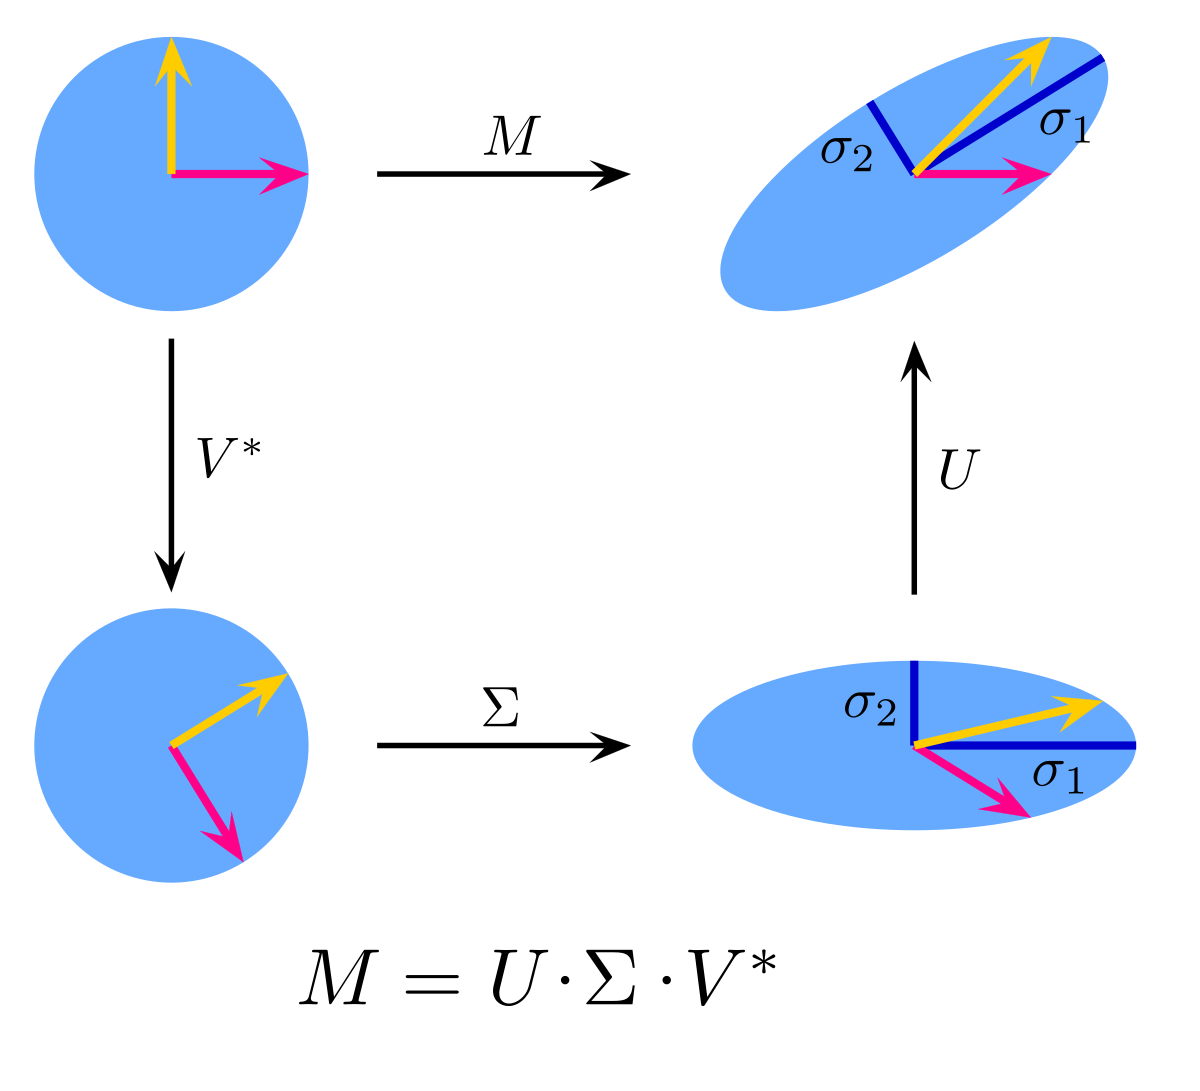
\includegraphics[scale=0.1]{figs/ln05/svd_geometry.png}
    \end{center}
    that SVD is, as priorly mentioned, a combination of three transformations. Where,
    \begin{bindenum}
        \item The orthonormal matrices $U$, $V$ are reflections or rotations.
        \item The matrix $\Sigma$ is a dilation.
    \end{bindenum}
    Furthermore, let us observe the vectors drawn on the unit circle. \\
    Since $V$ is orthonormal, we may conclude that $\vec{v_1} \perp \vec{v_2}$. However, bizzarely, we may also find that
    \[A \vec{v_1} \perp A \vec{v_2}\]
\end{ln-fig}

\section{Low Rank Approximation}
Low Rank Approximation is the task of approximating a matrix $A$ in a lower rank than $rk(A)$, to conserve computational cost and perform efficient computations.

\subsection{Matrix Norms}
Let us first discuss the optimization function of this task: matrix norm.

The norm of matrix also comes in diverse form, because matrices can be interpreted in many forms. \\
For example:
\begin{bindenum}
    \item Chunk of data (like an array)
    \item Operator of transformation
\end{bindenum}
Therefore, along these interpretations, we may present respective definitions of matrix norms.
\begin{ln-define}{Frobenius Norm}{}
    \textit{insert most recent COMPSCI 189 weeder homework PTSD.} \\
    The Frobenius Norm is defined as:
    \[
        \pnorm{A}{F} = \sqrt{\sum_{i = 1}^m \sum_{j = 1}^n A_{i,j}^2} = \sqrt{Trace(A^T A)}
    \]
    This is because the Frobenius inner product may be defined as:
    \[
        {\langle A, B \rangle}_F = Trace(A^T B) = \sum_{i = 1}^n \vec{A_i} \cdot \vec{B_i}
    \]
    and, as we recognize the relation between norm and inner product,
    \[
        \pnorm{A}{F} = \sqrt{{\langle A, A \rangle}_F} = \sqrt{\sum_{i = 1}^n \vec{A_i} \cdot \vec{A_i}}
    \]
\end{ln-define}
The Frobenius Norm has some interesting properties:
\begin{ln-theorem}{Orthonormal Matrices and Frobenius Norm}{}
    Let $U_1 \in \R^{m \times m}$, $A \in \R^{m \times n}$, and $U_2 \in \R^{n \times n}$, where $U_1, U_2$ are orthonormal. \\
    Then,
    \begin{align*}
        \pnorm{U_1 A}{F}
        &= \sqrt{Trace(A^T U_1^T U_1 A)} \\
        &= \sqrt{Trace(A^T A)} = \pnorm{A}{F} \\
        \pnorm{A U_2}{F}
        &= \sqrt{Trace(U_2^T A^T A U_2)} \\
        &\underset{\text{Commutivity in Trace}}{=} \sqrt{Trace(A^T A)} = \pnorm{A}{F} \\
    \end{align*}
\end{ln-theorem}
Now, let's discuss another definition of matrix norm:
\begin{ln-define}{Operator Norm (aka. Spectral Norm, L2-Norm)}{}
    Such norm is defined as:
    \[
        \pnorm{A}{2} = \max_{\pnorm{\vec{x}}{2} = 1} \pnorm{A \vec{x}}{2} = \sigma_{max}(A)
    \]
    \tcblower
    \textbf{Solution to Above Optimization Problem.}
    \begin{align*}
        \max_{\pnorm{\vec{x}}{2} = 1} \pnorm{A \vec{x}}{2}
        = \max_{\pnorm{\vec{x}}{2} = 1} \sqrt{\vec{x}^T A^T A \vec{x}}
        = \sqrt{\lambda_{max}(A^T A)} = \sigma_{max}(A)
    \end{align*}
    Suppose we attach another orthonormal matrix $U$ to the original matrix $A$, then the optimization problem develops a solution fairly similaly:
    \begin{align*}
        \max_{\pnorm{\vec{x}}{2} = 1} \pnorm{AU \vec{x}}{2}
        &= \max_{\pnorm{\vec{x}}{2} = 1} \sqrt{\vec{x}^T U^T A^T A U \vec{x}} \\
        &= \max_{\pnorm{\vec{x}}{2} = 1} \sqrt{\vec{y}^T A^T A \vec{y}} \\
        &= \sqrt{\lambda_{max}(A^T A)} = \sigma_{max}(A)
    \end{align*}
    where since we still find that $\vec{y}$ is normal, the attachment of $U$ providing no change to the optimization problem. \\
    Meanwhile, we find this phenomenon to persist even if $U$ is multiplied from an opposite direction:
    \begin{align*}
        \max_{\pnorm{\vec{x}}{2} = 1} \pnorm{UA \vec{x}}{2}
        &= \max_{\pnorm{\vec{x}}{2} = 1} \sqrt{\vec{x}^T A^T U^T U A \vec{x}} \\
        &= \max_{\pnorm{\vec{x}}{2} = 1} \sqrt{\vec{x}^T A^T A \vec{x}} \\
        &= \sqrt{\lambda_{max}(A^T A)} = \sigma_{max}(A)
    \end{align*}
    Therefore, we may also observe similar properties in norms, where:
    \[
        \pnorm{A}{2} = \pnorm{U_1A}{2} = \pnorm{AU_2}{2} \text{ for orthonormal matrices } U_1, U_2
    \]
\end{ln-define}


\newpage
\chapter{Low-Rank Approximation}

\section{Discussion of L-RA}
Suppose we have some matrix $A \in \R^{m \times n}$, where storing this matrix would take significant computational resources.
Is there a method to store an approximation of this matrix, such that the approximation is more efficient to store for, and we would thus reduce computational cost of storage? \\
We have discussed the possibility of such technique within the previous lecture, where we have solved the optimization problem:
\[\max_{\pnorm{\vec{x}}{2} = 1} \pnorm{A \vec{x}}{2}\]

Today, we will discuss the extension of such solution: Low-Rank Approximation. \\
It would be characterized from the optimization problem:
\[
    \underset{B \in \R^{m \times n}, rk(B) = k}{\text{argmin}} \pnorm{A - B}{F}
\]
where we may see a contextually similar optimization problem:
\[
    \underset{B \in \R^{m \times n}, rk(B) = k}{\text{argmin}} \pnorm{A - B}{2}
\]
Let us perform a proof on this:
\begin{ln-explain}{The LRA Optimization Problem on Spectral Norm}{}
    \textbf{Problem.}
    \[
        \underset{B \in \R^{m \times n}, rk(B) = k}{\text{argmin}} \pnorm{A - B}{2}
    \]
    \tcblower
    \textbf{Solution.} \\
    Keep in mind that our proof proceeds in the direction of:
    \begin{bindenum}
        \item Finding a possible upper bound
        \item Finding the achievability of such upper bound
        \item Finding the legitimacy of such upper bound
    \end{bindenum}
    Now, let us move on with the subparts of a proof. \\
    \par
    \textbf{\textit{Finding a Possible Upper Bound.}} \\
    Let us define
    \[
        A_k = \sum_{i = 1}^k \sigma_i \vec{u_i} \vec{v_i}^T
    \]
    Then, the difference between such approximation and $A$ would be:
    \[\pnorm{A - A_k}{2} = \pnorm{A_n - A_k}{2} = {\Bigg\| \sum_{i = k + 1}^n \sigma_i \vec{u_i} \vec{v_i}^T \Bigg\|}_2\]
    which, following along the optimization problem phrased last lecture, we would obtain the solution to be:
    \[
        {\Bigg\| \sum_{i = k + 1}^n \sigma_i \vec{u_i} \vec{v_i}^T \Bigg\|}_2 = \sigma_{k + 1} (A)
    \]
    \par
    \textbf{\textit{Finding the Legitimacy (and Achievability) of Upper Bound.}} \\
    Then, let us show that for every $B$ where $rk(B) \leq k$, the difference $\pnorm{A - B}{2}$ is larger than our current possible minimum, $\sigma_{k + 1}$. By proving so we secure the result of maximization is as illustrated above. \\
    Let us first define $\vec{w}$ that,
    \[
        \pnorm{A - B}{2} = \max_{\pnorm{\vec{w}}{} = 1} \pnorm{(A - B) \vec{w}}{2}
    \]
    Where, if $\vec{w} \in N(B)$, then we would be able to simplify the above optimization problem into something easier to solve: along such above constraint, let us note that,
    \[
        \pnorm[2]{A - B}{2} \geq \pnorm[2]{(A - B) \vec{w}}{2} = \pnorm[2]{A \vec{w}}{2}
    \]
    And decomposing $A$ into SVD form, which contains orthonormal matrices,
    \[
        \pnorm[2]{A - B}{2} \geq \pnorm[2]{U \Sigma V^T \vec{w}}{2} = \pnorm[2]{\Sigma V^T \vec{w}}{2}
    \]
    Provided that $\vec{w}$ is a unit vector, and $V$ is invertible, we can guarantee that
    \[
        \exists \vec{a}, V \vec{a} = \vec{w}
    \]
    Therefore, let us now substitute such value in, and we will obtain that
    \begin{align*}
        \pnorm[2]{A - B}{2}
        &\geq \pnorm[2]{\Sigma V^T \vec{w}}{2} \\
        &= \pnorm[2]{\Sigma \vec{a}}{2} \\
        &= \vec{a}^T \Sigma^T \Sigma \vec{a} = \vec{a}^T \Lambda \vec{a}
    \end{align*}
    Let us come back to our assumption that $\vec{w} \in N(B)$, and extract more insights from it. \\
    Now, we may define along the $V$ of $A = U \Sigma V^T$ that:
    \[
        V_{k + 1} = \begin{bmatrix} \vec{v}_1 & \cdots & \vec{v}_{k + 1}\end{bmatrix}
    \]
    where along the property of SVD we understand that $rk(V_{k + 1}) = k + 1$. \\
    To find some $\vec{w}$ such that $\vec{w} \in N(B) \land \vec{w} \in \mathcal{R}(V_{k + 1})$, we should notice that:
    \begin{enumerate}
        \item Along rank-nullity theorem, $\dim(N(B)) \geq n - k$.
        \item Along above description, $\dim(R(V_{k + 1})) = k + 1$
    \end{enumerate}
    At this point, we must note that the achievability in our proposed upper bound exists in the possibility of having such $\vec{w}$. Therefore, \textbf{the achievability of upper bound is protected by the existence of $\vec{w}$, which we must guarantee}. \\
    These two subspaces of $\R^n$ must have overlap. Therefore, there must exist some vector that belongs to both subspaces. This guarantees the existence of our $\vec{w}$.
    \par
    \textbf{\textit{Back to the Achievability of Upper Bound, Final Step}}. \\
    Let us now follow along, and revisit the derivation that $\vec{a} = V^T \vec{w}$ on the change of basis. \\
    Then, here we perform the final computations:
    \begin{align*}
        \vec{a} &= V^T \vec{w} \\
        &= V^T (\sum_{i = 1}^{k + 1} a_i \vec{V}_i) \\
        &= \begin{bmatrix} a_1 & \cdots & a_{k + 1} & 0 & \cdots & 0 \end{bmatrix}^T \\
        \vec{a}^T \Lambda \vec{a}
        &= \sum_{i = 1}^{k + 1} a_{i}^2 \lambda_i \\
        &\geq \sum_{i = 1}^{k + 1} a_{i}^2 \lambda_{k + 1} = \lambda_{k + 1} \sum_{i = 1}^{k + 1} a_{i}^2 \\
        &= \lambda_{k + 1} = \sigma_{k + 1}^2 \textit{(Note, $\mathit{\pnorm{\vec{a}}{2} = \pnorm{\vec{w}}{2} = 1}$)}
    \end{align*}
\end{ln-explain}

\begin{ln-explain}{The LRA Optimization Problem on Frobenius Norm}{}
    \textbf{Problem.}
    \[
        \underset{B \in \R^{m \times n}, rk(B) = k}{\text{argmin}} \pnorm{A - B}{F}
    \]
    \tcblower
    \textbf{Solution.} \\
    Let us consider $A_k$ as priorly defined to be the solution of optimization again.
    \begin{align*}
        \pnorm[2]{A}{F} &= \pnorm[2]{U \Sigma V^T}{F} \\
        &= \pnorm[2]{\Sigma}{F} = \sum_{i = 1}^n \sigma_i^2 \\
        \pnorm[2]{A - A_k}{F} &= \sum_{i = k + 1}^n \sigma_i^2 \\
        \pnorm[2]{A - B}{F} &= \sum_{i = 1}^n \sigma_i^2 (A - B)
    \end{align*}
    Now, following the logic before, we want to prove this upperbound:
    \begin{quote}
        Prove that $\forall B \in \R^{m \times n}\ s.t.\ rk(B) = k, \pnorm{A - B}{F} \geq \pnorm{A - A_k}{F}$
    \end{quote}
    Using the aligned equations above, let us find an equivalent proof prompt,
    \begin{quote}
        Prove that $\forall i, \sigma_i (A - B) \geq \sigma_{k + i}(A)$
    \end{quote}
    Where, along spectral norm's definition, we can also obtain that,
    \[
        \sigma_{k + 1}(A) = \pnorm{A - A_{k + i - 1}}{2}
    \]
    translated in text stating that $A_{k + i - 1}$ is the best rank $(k + i - 1)$ approximation to $A$ in spectral norm sense. \\
    Now, let us return to the above equivalent prompt and define such that $C := A - B$.
    \begin{align*}
        \sigma_i (A - B)
        &= \sigma_i (C) \\
        &= \pnorm{C - C_{i - 1}}{2} = \pnorm{A - B - C_{i - 1}}{2}
    \end{align*}
    Pay attention to the rank of these matrices:
    \begin{align*}
        B = B_k, &rk(B_k) \leq k \\
        rank(C_{i - 1}) \leq i - 1 \\
        rk(B_k + C_{i - 1}) \leq k + i - 1
        \sigma_i (A - B) &= \pnorm{A - D}{2}\\
        &, where\ rk(D) \leq k + i - 1
    \end{align*}
    Using the solution from spectral norm side proof of LRA,
    \begin{align*}
        \pnorm{A - D}{2} \geq \pnorm{A - A_{k + i - 1}}{2} = \sigma_{k + 1} (A)
    \end{align*}
\end{ln-explain}

\newpage
\chapter{Vector Calculus}
The motivation of vector calculus is to work with linear algebra problems more analytically, in more interpretable methods. \\
The tools that help to optimize linear algebra expression is the calculus of vector: vector calculus.

\section{Function Expansion: Taylor Series}
Let's start with functions, the basic of calculus.
\begin{ln-define}{Scalar Valued Function of Vector}{}
    Let a function $f$ be such that:
    \[
        f(\vec{x}): \R^n \rightarrow \R
    \]
    Such a function is by definition a scalar valued function of vector.
\end{ln-define}
Then, we may begin our effort to generalize the derivative of such functions, as follows.

First of all, let us recap Calculus II knowledge of polynomial expansion of some fucntion:
\begin{ln-theorem}{Taylor's Theorem (Expansion)}{}
    Let $f$ be a scalar valued function for scalar:
    \[
        f(x) : \R \rightarrow \R, x_0 \in \R
    \]
    Then, Taylor expansion allows us to write such that:
    \[
        f(x_0 + \Delta x) = f(x_0) + \dv{f}{x} \bigg|_{x = x_0} \Delta x + \cdots
    \]
    Essentially, 
    \[
        f(x_0 + \Delta x) = \sum_{i = 0}^n \frac{f^{(i)}(x_0) {(\Delta x)}^i}{i!}
    \]
    where we call the Taylor expansion towards the $n^{th}$ degree term be an $n^{th}$ order Taylor expansion.
\end{ln-theorem}
What is the purpose of introducing Taylor's expansion here? The fact is, we may approximate a value $f(x_0 + \Delta x)$ based on $f(x)$ along the product of $\Delta x$ and a derivative.
\textbf{The derivative affects how large the ``perturbation'' is that occurs in the approximation of $f(x_0 + \Delta x)$}.
Similar logic is applied for upcoming $n$-order derivatives.

Then, along the above reintroduction of Taylor's Series, let us look at a vector edition of Taylor's Theorem:
\begin{ln-theorem}{Taylor's Theorem for Vectors}{}
    Let $f$ be a scalar valued function for vector. \\
    Then, we may express that:
    \begin{align*}
        f(\vec{x_0} + \Delta \vec{x})
        &= f(\vec{x_0}) + \pdv{f}{x} \bigg|_{\vec{x} = \vec{x_0}} \Delta \vec{x} + \frac{1}{2!} {(\Delta \vec{x})}^T \nabla^2 f(\vec{x}) \bigg|_{\vec{x} = \vec{x_0}} \Delta \vec{x}
    \end{align*}
\end{ln-theorem}
We usually stop at the second order approximation when using Taylor's Theorem for vectors, because this is usually a good equilibrium point for computational precision and simplification.

\section{Function Expansion: Derivative of Vector Functions}
In addition, we define the derivative of vectors as follows:
\begin{ln-define}{Derivatives of Scalar Valued Vector Function}{}
    Here, we observe that the first order derivative of such functions are row vectors, and the second order derivative is a matrix called \textbf{Hessian}:
    \begin{align*}
        \pdv{f}{x} = {(\nabla_{\vec{x}}f)}^T &= \begin{bmatrix} \pdv{f}{x_1} & \cdots & \pdv{f}{x_n} \end{bmatrix} \\
        {(\nabla^2 f(\vec{x}))}_{i,j} &= \pdv{f}{x_i}{x_j} \\
        \nabla^2 f(\vec{x}) &\in \mathbb{S}^n
    \end{align*}
\end{ln-define}
Note that it is only for convex functions where the symmetric argument of Hessian applies. \\
This is beacuse:
\[
    \pdv{f}{x_i}{x_j} = \pdv{f}{x_i} \pdv{f}{x_j}
\]
where the order of variables put matters for functions. \\
The reason why convex functions can host the symmetric Hessian is because of Clairaut's Theorem (not explicitly mentioned in lecture):
\begin{ln-theorem}{Clairaut's Theorem}{}
    If the second partial derivatives of a function are continuous, then the order of differentiation is immaterial. \\
    Alternatively (quoted from Purdue University),
    \begin{quote}
        Let $f : \R^2 \rightarrow \R$ have all partial derivatives up to second derivative be continuous near $(a, b)$, then:
        \[
            \pdv{f}{x}{y} (a, b) = \pdv{f}{y}{x} (a, b)
        \]
    \end{quote}
\end{ln-theorem}

\subsection{Examples of Polynomial Expansion}
Now, let us provide an example in approximating a scalar valued vector function via Taylor's Theorem:
\begin{ln-explain}{Polynomial Expansion of 2-Norm}{}
    Let us attempt to find a Taylor Expansion for the function
    \[f(\vec{x}) = \pnorm[2]{\vec{x}}{2}\]
    We will define the level sets of this function as:
    \[
        \{\vec{x} \big| f(\vec{x}) = C\}
    \]
    which would be circles centered at the origin with radius $\sqrt{C}$. \\
    The gradient of such function would be:
    \[
        \nabla_{\vec{x}}f = \begin{bmatrix} 2x_1 \\ 2x_2 \end{bmatrix}
    \]
    And the Hessian:
    \[
        H_{\vec{x}}f = \begin{bmatrix} 2 & 0 \\ 0 & 2 \end{bmatrix}
    \]
    Therefore, upon Taylor's Theorem,
    \begin{align*}
        f(\vec{x_0} + \Delta \vec{x})
        &= f(\vec{x_0}) + {(\nabla_{\vec{x}}f)}^T \Delta \vec{x} + \frac{1}{2!} {(\Delta \vec{x})}^T H_{\vec{x}}f \Delta \vec{x} \\
        &= {x_0}_1^2 + {x_0}_2^2 + 2{x_0}_1 \Delta x_1 + 2{x_0}_2 \Delta x_2 + {(\Delta x_1)}^2 + {(\Delta x_2)}^2 \\
        &= {({x_0}_1 + \Delta x_1)}^2 + {({x_0}_2 + \Delta x_2)}^2 = \pnorm[2]{\vec{x_0} + \Delta \vec{x}}{2}
    \end{align*}
\end{ln-explain}
Since the Hessian is symmetric, we can perform a lot of interesting mathematics with it. \\
A third order derivative is known as a tensor, but this is out of scope for EECS 127.

Let's look at some more examples of Taylor Expansion:
\begin{ln-explain}{Polynomial Expansion of Euclidean Inner Product}{}
    Let us find a Taylor Expansion to the function:
    \[
        f(\vec{x}) = \vec{x}^T \vec{a}, \vec{a} \in \R^n
    \]
    The gradient of such function is then,
    \[
        \nabla_{\vec{x}} f = \vec{a}
    \]
    Then, the Hessian of such function would be a zero matrix. \\
    Therefore,
    \begin{align*}
        f(\vec{x_0} + \Delta \vec{x})
        &= f(\vec{x_0}) + {(\nabla_{\vec{x}} f)}^T \Delta \vec{x} \\
        &= \sum_{i = 1}^n a_i ({x_0}_i + \Delta x_i) = {(\vec{x_0} + \Delta \vec{x})}^T \vec{a}
    \end{align*}
\end{ln-explain}


\subsection{Matrix in Vector Calculus}
Let us discuss how the roles of matrices are when we take the derivative of a scalar-valued function by a vector.
\begin{ln-explain}{Derivatives of Matrix-Involving Inner Product}{}
    Let us find the derivative expressions to the function:
    \[
        f(\vec{x}) = \vec{x}^T A \vec{x}, A \in \R^{n \times n}
    \]
    We can derive the gradient as follows:
    \begin{align*}
        \frac{\partial}{\partial x_i} \vec{x}^T A \vec{x}
        &= \frac{\partial}{\partial x_i} \vec{x}^T \begin{bmatrix} \vec{A_1} & \cdots & \vec{A_n} \end{bmatrix} \vec{x} \\
        &= \frac{\partial}{\partial x_i} \begin{bmatrix} \vec{x} \cdot \vec{A_1} & \cdots & \vec{x} \cdot \vec{A_n} \end{bmatrix} \vec{x} \\
        &= \frac{\partial}{\partial x_i} \sum_{k = 1}^n \sum_{j = 1}^n A_{j, k} x_k x_j \\
        &= \frac{\partial}{\partial x_i} \bigg( \sum_{j = 1}^n A_{j, i} x_i x_j + \sum_{k = 1}^n A_{i, k} x_i x_k \bigg) \\
        &= \sum_{j = 1}^n A_{j, i} x_j + \sum_{k = 1}^n A_{i, k} x_k
        = \vec{(A^T)}_i \cdot \vec{x} + \vec{A}_i \cdot\vec{x} \\
        \frac{\partial}{\partial x} \vec{x}^T A \vec{x} &= (A + A^T) \vec{x}
    \end{align*}
    And, uh, Hessians.
    \begin{align*}
        \nabla^2 f(\vec{x})
        &= \frac{\partial}{\partial x} (A + A^T) \vec{x} = A + A^T
    \end{align*}
\end{ln-explain}

Then, let us define the derivative of a vector-valued function with respect to some vector variable:
\begin{ln-define}{Jacobian (Derivative) of Vector-Valued Vector Function}{}
    For some function $f(\vec{x}) = \vec{y}$ such that:
    \[
        f: \R^n \rightarrow \R^m
    \]
    Then,
    \[
        J = \begin{bmatrix} \pdv{\vec{f}}{x_1} & \cdots & \pdv{\vec{f}}{x_n} \end{bmatrix}
    \]
\end{ln-define}

\begin{ln-explain}{The Jacobian of Polar-Cartesian Coordinate Translator}{}
    Let $f$ be the function:
    \[
        f(\vec{v}) = \begin{bmatrix} r \cos(\theta) \\ r \sin(\theta) \end{bmatrix}
    \]
    Then the Jacobian of it would be:
    \[
        J =
        \begin{bmatrix}
            \cos(\theta) & -r \sin(\theta) \\
            \sin(\theta) & r \cos(\theta)
        \end{bmatrix}
    \]
    whose determinant would then be $\det(J) = r$.
\end{ln-explain}

Last but not least, let us explore chain rule in matrix calculus:
\begin{ln-define}{Chain Rule}{}
    Let a function $f$ be
    \[
        f(\vec{x}) = g(h(\vec{x}))
    \]
    Then, we may express that
    \[
        \dv{f}{x} = \dv{g}{y} \dv{h}{x}
    \]
    \tcblower
    \textbf{Example.} \\
    Now, let's look at the least squares problem. \\
    Originally, we perform this computation:
    \begin{align*}
        f(x)
        &= \pnorm[2]{A \vec{x} - \vec{b}}{2} \\
        &= {(A \vec{x} - \vec{b})}^T ((A \vec{x} - \vec{b})) \\
        &= \vec{x}^T A^T A \vec{x} - 2 \vec{x}^T A \vec{b} + \vec{b}^T \vec{b} \\
        \nabla_{\vec{x}} f(\vec{x})
        &= (A^T A + A^T A) \vec{x} - 2 A^T \vec{b} \\
        &= 2 A^T A \vec{x} - 2 A \vec{b} \\
        \vec{x}^* &= {(A^T A)}^{-1} A^T \vec{b}
    \end{align*}
    Instead, we may use chain rule:
    \begin{align*}
        \dv{f}{x}
        &= \dv{g}{y} \dv{h}{x} \\
        &= {(\nabla_{\vec{y}} g)}^T \dv{}{x} {} (A \vec{x}) \\
        &= 2(A \vec{x} - \vec{b})^T \cdot A
    \end{align*}
    We may thus obtain the gradient to be:
    \[
        \nabla_{\vec{x}} f = 2 A^T (A \vec{x} - \vec{b})
    \]
\end{ln-define}

\newpage
\chapter{The Extension of Vector Calculus}
\textit{Note: This lecture's content will be shorter than other notes because half of the lecture was put on reviewing MATH 53 (as written in Lecture 7)}

\section{The Main Theorem}
The. Main. 
\begin{ln-theorem}{The Main Theorem}{}
    \textbf{Theorem.} Let $\Omega$ be an open subset of $\R^n$, and let function $f$ be differentiable and such that
    \[
        f : \R^n \rightarrow \R
    \]
    then, for an optimal solution $\vec{x}^*$ that solves the optimization problem:
    \[
        \min_{\vec{x} \in \Omega} f(\vec{x})
    \]
    Then, the Main Theorem states that,
    \[
        \dv{f}{\vec{x}} \big|_{\vec{x} = \vec{x}^*} = 0
    \]
    \tcblower
    \textbf{Proof.} 
    We realize that $\Omega$ is an open set, meaning $\vec{x}^* + \Delta \vec{x}$ can be guaranteed to be involved in $\Omega$, for the definition of an open set is such that,
    \[\forall x \in \Omega, \exists \epsilon > 0 \ (|x - y| < \epsilon \implies y \in \Omega)\]
    Then, by the Taylor expansion and optimality assumption, we may state that:
    \begin{align*}
        f(\vec{x}^* + \Delta \vec{x}) &= f(\vec{x}^*) + \dv{f}{x} \bigg|_{\vec{x} = \vec{x}^*} (\Delta \vec{x}) + \frac{1}{2} {(\Delta \vec{x})}^T \dv[2]{f}{x} \bigg|_{\vec{x} = \vec{x}^*} (\Delta \vec{x}) \geq f(\vec{x}^*)
    \end{align*}
    Manipulating the above inequality,
    \begin{align*}
        \dv{f}{x} \bigg|_{\vec{x} = \vec{x}^*} (\Delta \vec{x}) &+ \frac{1}{2} {(\Delta \vec{x})}^T \dv[2]{f}{x} \bigg|_{\vec{x} = \vec{x}^*} (\Delta \vec{x}) &&\geq 0 \\
        \dv{f}{x} \bigg|_{\vec{x} = \vec{x}^*} &+ \frac{sum(H.O.T.)}{\Delta \vec{x}} &&\geq 0 \\
        \lim_{\Delta \vec{x} \rightarrow 0} \bigg( \dv{f}{x} \bigg|_{\vec{x} = \vec{x}^*} &+ \frac{sum(H.O.T.)}{\Delta \vec{x}} \bigg) = \dv{f}{x} \bigg|_{\vec{x} = \vec{x}^*} &&\geq 0
    \end{align*}
    We may then provide a symmetric argument on the value $\vec{x}^* - \Delta \vec{x}$:
    \begin{align*}
        - \dv{f}{x} \bigg|_{\vec{x} = \vec{x}^*} (\Delta \vec{x}) &+ \frac{1}{2} {(\Delta \vec{x})}^T \dv[2]{f}{x} \bigg|_{\vec{x} = \vec{x}^*} (\Delta \vec{x}) &&\geq 0 \\
        - \dv{f}{x} \bigg|_{\vec{x} = \vec{x}^*} &+ \frac{sum(H.O.T.)}{\Delta \vec{x}} &&\geq 0 \\
        \lim_{\Delta \vec{x} \rightarrow 0} - \bigg( \dv{f}{x} \bigg|_{\vec{x} = \vec{x}^*} &+ \frac{sum(H.O.T.)}{\Delta \vec{x}} \bigg) = - \dv{f}{x} \bigg|_{\vec{x} = \vec{x}^*} &&\geq 0 \\
    \end{align*}
    \[
        \dv{f}{x} \bigg|_{\vec{x} = \vec{x}^*} \leq 0
    \]
    Consequently, we reach the following conclusion:
    \[
        \dv{f}{x} \bigg|_{\vec{x} = \vec{x}^*} \geq 0 \land \dv{f}{x} \bigg|_{\vec{x} = \vec{x}^*} \leq 0 \implies \dv{f}{x} \bigg|_{\vec{x} = \vec{x}^*} = 0 
    \]
    \textit{Note: H.O.T. means ``Higher Order Terms'' of Taylor Expansion, starting from the second-order term}
\end{ln-theorem}

\section{Perturbation Analysis, Effect of Noise}
In this problem, we consider the following concern:
\begin{quote}
    Let $A \vec{x} = \vec{y}$, where $A$ is a square invertible matrix. \\
    Then, for some change in $\vec{y}$ (characterized as $\Delta \vec{y}$), how would this affect $\vec{x}$?
    \par
    In other words, we compare $\frac{\pnorm{\Delta \vec{x}}{2}}{\pnorm{\vec{x}}{2}}$ with $\frac{\pnorm{\Delta \vec{y}}{2}}{\pnorm{\vec{y}}{2}}$
\end{quote}
Let us now set up the problem:
\begin{ln-explain}{Formulating the Perturbation Analysis}{}
    Let us see that,
    \begin{align*}
        A \vec{x} &= \vec{y} \\
        A (\vec{x} + \Delta \vec{x}) &= \vec{y} + \Delta \vec{y}
    \end{align*}
    Then, we may manipulate the expressions to find that,
    \begin{align*}
        A \Delta \vec{x} = \Delta \vec{y} \implies \Delta \vec{x} &= A^{-1} \Delta \vec{y} \\
        \pnorm{\Delta \vec{x}}{2} &= \pnorm{A^{-1} \Delta \vec{y}}{2} \leq \pnorm{A^{-1}}{2} \pnorm{\Delta \vec{y}}{2}
    \end{align*}
    The last line is certified because the spectral norm of $A^{-1}$ measures how much can it transform the norm of a vector.
    \par
    Then, we may provide a minimization problem:
    \[
        \min \frac{\pnorm{\Delta \vec{x}}{2}}{\pnorm{\vec{x}}{2}}
    \]
    Now, let us observe the following work of upperbounding such denominator:
    \begin{align*}
        A \vec{x} = \vec{y} &\implies \pnorm{A \vec{x}}{2} \leq \pnorm{A}{2} \pnorm{\vec{x}}{2} \\
        \pnorm{\vec{y}}{2} &\leq \pnorm{A}{2} \pnorm{\vec{x}}{2} \\
        \pnorm{\vec{x}}{2} &\geq \frac{\pnorm{\vec{y}}{2}}{\pnorm{A}{2}}
    \end{align*}
    And therefore,
    \begin{align*}
        \frac{\pnorm{\Delta \vec{x}}{2}}{\pnorm{\vec{x}}{2}}
        &\leq \pnorm{A^{-1}}{2} \pnorm{\vec{y}}{2} \frac{\pnorm{A}{2}}{\pnorm{\vec{y}}{2}} \\
        &= \pnorm{A^{-1}}{2} \pnorm{A}{2} \frac{\pnorm{\Delta \vec{y}}{2}}{\pnorm{\vec{y}}{2}} \\
        &= \sigma_{\max}(A) \sigma_{\max}(A^{-1}) \frac{\pnorm{\Delta \vec{y}}{2}}{\pnorm{\vec{y}}{2}}
        = \frac{\sigma_{\max}(A)}{\sigma_{\min}(A)} \frac{\pnorm{\Delta \vec{y}}{2}}{\pnorm{\vec{y}}{2}}
    \end{align*}
    Consequently, we arrive at the conclusion (summary) of:
    \[
        \frac{\pnorm{\Delta \vec{x}}{2}}{\pnorm{\vec{x}}{2}} \leq \frac{\sigma_{\max}(A)}{\sigma_{\min}(A)} \frac{\pnorm{\Delta \vec{y}}{2}}{\pnorm{\vec{y}}{2}}
    \]
    where we call the fraction $\frac{\sigma_{\max}(A)}{\sigma_{\min}(A)}$ the \textbf{condition number}.
\end{ln-explain}

\newpage
\chapter{Ridge Regression}

\section{Perturbation Analysis Guides into Ridge Regression}
In the concept of perturbation analysis, we ask that, for some system
\[A \vec{x} = \vec{y}\]
with a square, invertible $A$, how much would $\vec{x}$ change provided some small change $\vec{y} \rightarrow \vec{y} + \vec{\partial y}$?

Then, our solution (cited in Chapter 8, or Lecture 8) is as follows:
\[
    \frac{\pnorm{\vec{\partial x}}{2}}{\pnorm{\vec{x}}{2}} \leq \frac{\sigma_{\max}(A)}{\sigma_{\min}(A)} \frac{\pnorm{\vec{\partial y}}{2}}{\pnorm{\vec{y}}{2}}
\]
From whcich, we discover the characteristic of a matrix called \textbf{condition number}:
\[\frac{\sigma_{\max}(A)}{\sigma_{\min}(A)}\]

Let us connect the above discussion to the Least Squares Problem. \\
In the context of least squares problem, we are provided a more robust normal equation via the use of pseudoinverse:
\[
    (A^\dagger A) \vec{x} = A^T \vec{b}
\]
As our least square system is sensitive to noise, we may investigate the condition number of $A^T A$ to observe the system's change in its solution provided the perturbation in system measurements. \\
This is significant in computations. A high condition number makes a system's matrix highly unstable for numerical precisions to persist provided noise in measurements and systems.
Such property is, in fact, demonstrated by the convergence warnings in Jupyter iPython notebooks!
\par
But, provided the significance of condition number, we may also discuss ways to alleviate its problems.
To reduce the condition number of some matrix, we may attempt to reduce the ratio of singular values via adding some multiple of identity matrix ($\lambda I$) to it.
This allows us to greatly reduce the condition number, shifting it away from instability and being less prone to variance in training data:
\[A^T A + \lambda I\]
As a side note, in CS189, we discover similar approaches that can help tackle training data that leads to singular covariance matrices. \\
Let us investigate below why adding a multiple of diagonal matrix does not make our regression problem have a very deviated solution (despite the fact we somehow alter the design matrix of our problem).

\section{Ridge Regression}
In the least squares problem, we have a formulated optimization problem of:
\[
    \min_{\vec{x}} \pnorm{A \vec{x} - \vec{b}}{2}
\]
to offer insight to the optimization problem to prevent its divergence from true parameter value, is to present a new formulation of the problem:
\[
    \min_{\vec{x}} \pnorm[2]{A \vec{x} - \vec{b}}{2} + \lambda^2 \pnorm[2]{\vec{x}}{2}
\]
where, we regularize the least squares solution by stating that large solutions of $\vec{x}$ must lead to unidealistic increase in the cost (loss) function.
We penalize a large least squares solution $\vec{x}$.

Here, using different norms in the regularizer will provide different properties.
The L1 regularizer has the LASSO property (as outlined in DATA C100), while the L2 regularizer we use now provides a convex function as well as a closed-form solution unlike the L1 effort (once again, as outlined in DATA C100).

Let us first compute the gradient of such loss function:
\begin{align*}
    \nabla_{\vec{x}} \pnorm[2]{A \vec{x} - \vec{b}}{2} + \lambda^2 \pnorm[2]{\vec{x}}{2}
    &= 2A^T (A \vec{x} - \vec{b}) + 2 \lambda^2 I \vec{x} \\
    \vec{x}^* &= {(A^T A + \lambda^2 I)}^{-1} A^T \vec{b}
\end{align*}
The eigenvalues of $A^T A + \lambda^2 I$, meanwhile, would be the eigenvalues of $A^T A$ added the value $\lambda^2$ (by manipulating the definition of eigenvalues and eigenvectors). \\
This is also known as the shift property of eigenvalues:
\begin{ln-theorem}{Shift Property of Eigenvalues}{}
    Let $\vec{v}$ be an eigenvector of $A^T A$. \\
    Then, provided that:
    \[
        A^T A \vec{v} = \mu \vec{v}
    \]
    we may see that,
    \[
        (A^T A + \lambda^2 I) \vec{v} = (\mu + \lambda^2) \vec{v}
    \]
    Thus determine that:
    \begin{quote}
        for any eigenpair of $A^T A$ being $(\mu, \vec{v})$, a corresponding eigenpair exists in $A^T A + \lambda^2 I$ being $(\mu + \lambda^2, \vec{v})$.
    \end{quote}
\end{ln-theorem}
Therefore, small $\lambda$ corresponds to less regularizaiton effort, and vice versa.

\subsection{Development of Ridge Regression}
Now, suppose we have a least square system where $\vec{x}$ has a smaller norm, where $\lambda I \vec{x} \sim \vec{0}$. \\
Then, by that close-to-zero property we observe in $\lambda I \vec{x}$, adding the information of $\lambda I$ into the least squares problem formulation would barely alter the original formulation too much, due to the close-to-zero-ness of ridge regression's current least squares solution. \\
This allows us to use larger $\lambda$ (have greater regularization). \\
We have two ways of incorporating such information into the least squares problem now:
\begin{bindenum}
    \item Vertically concatenate $\lambda I$ below $A$.
    \item Use Ridge Regression's format, which uses a similar idea to preserve the original system as much as possible. We will prove later that this is exactly the first idea.
\end{bindenum}
In the concatenation idea, our system of least squares problem is reformulated as:
\[
    \begin{bmatrix} A \\ \lambda I \end{bmatrix} \vec{x} = \begin{bmatrix} \vec{b} \\ \lambda I \vec{x} \end{bmatrix}
\]
Let's use both block matrix and normal equation to further explore the idea of concatenating $\lambda I$:
\begin{align*}
    &{\bigg( \begin{bmatrix} A^T & \lambda I \end{bmatrix} \begin{bmatrix} A \\ \lambda I \end{bmatrix} \bigg)}^{-1}
    \begin{bmatrix} A^T & \lambda I \end{bmatrix} \begin{bmatrix} \vec{b} \\ \lambda I \vec{x} \end{bmatrix} \\
    &= (A^T A + \lambda^2 I) (A^T \vec{b} + \lambda^2 I \vec{x}) \\
    &\sim (A^T A + \lambda^2 I) A^T \vec{b}
\end{align*}
and we have therefore demonstrated the similarity between the two ideas of ridge regression. \\
It is noteworthy that the common notation of ridge regression does not use the notation $\lambda^2$ when addressing regularization parameter.
We are doing so in the context of demonstrating how ridge regression is developed, through a simpler set of mathematical notations.
\par
Once we expand the idea to adding weights for matrices, creating the system:
\[
    \begin{bmatrix} W_1 A \\ W_2 I \end{bmatrix} \vec{x} = \begin{bmatrix} W_1 \vec{b} \\ W_2 \vec{x_0} \end{bmatrix}
\]
we end up with a new optimization problem:
\[
    \min_{\vec{x}} \pnorm[2]{W_1 (A \vec{x} - \vec{b})}{2} + \pnorm[2]{W_2 (\vec{x} - \vec{x_0})}{2}
\]
which we call the \textbf{Tikhonov Regularization} technique. \\
\textit{Note: $\vec{x_0}$ is an arbitrary piece of information.}

\section{Probabilistic Information from Ridge Regression}
Suppose that we instead now have probabilistic information:
\[
    (\vec{x_i}, y_i), \text{ where } y_i = g(x_i) + z_i
\]
and, $z_i \sim \mathcal{N}(0, \sigma_i^2)$ is a noise defined on a Gaussian distribution. \\
And, suppose we have a linear model,
\[
    y_i = \vec{w}^T \vec{x} + z_i
\]
Then, we may state that,
\[
    f_{z_i} (z_i) = \frac{\exp(-\frac{z_i^2}{2\sigma_i^2})}{\sqrt{2 \pi} \sigma_i}
\]
and we attempt to learn the weights $\vec{w}$ to complete the model for some related problem. \\
Therefore, with multivariate Gaussian noise $\vec{z}$ and datapoint matrices $X$, we formulate this as a least square system,
\[
    X \vec{w} + \vec{z} = \vec{y}
\]

\subsection{Maximum Likelihood Estimation and Maximum A-Posteriori}
Now, we may attempt to estimate the parameters that makes the observed data most likely. \\
This is related to the technique of Maximum Likelihood Estimation. Let me shamelessly copy a segment of my CS189 notes here to provide a brief explanation:
\begin{ln-explain}{MLE from CS189}{}
    Suppose that we go back to the coin flip example (just like 126 does), where heads appear with a probability $p$ (and otherwise for tails). \\
    Then, statisticians world ask, provided the real data of coin, what value of $p$ (the parameter of coin flip probability distribution) is closest to its true inherent value.

    Let us suppose that the number of heads we obtain is a discrete random variable, $X \sim Binomial(n, p)$:
    \[
        \P(X = x) = \binom{n}{x} p^x {(1 - p)}^{n - x}
    \]
    Then, let us propose that the real data presents $k$ heads, and we would defined the Likelihood function $\mathcal{L}$ as:
    \[
        \mathcal{L}(p) = \P(X = k) = \binom{n}{k} p^k {(1 - p)}^{n - k}
    \]
    where it is a function of distribution parameters.
\end{ln-explain}
Then, Maximum Likelihood Estimation (MLE) is the method of estimating the parameters of a statistical distribution by picking the parameters that maximize $\mathcal{L}$.
Furthermore, it would be a method of density estimation, where we estimate some probability density function from the provided dataset.
\par
In this case, we are performing MLE to obtain weight $\vec{w}$ provided the Gaussian noise $\vec{z}$:    
\begin{ln-explain}{Solving Maximum Likelihood Estimation Phrased Optimization}{}
    Let us begin from the prompt:
    \begin{align*}
        \underset{\vec{w}_0}{\rm argmax}\ f (\vec{y} | \vec{w} = \vec{w_0})
        &= \underset{\vec{w}_0}{\rm argmax}\ \prod_{i = 1}^n f(Y_i = y_i | \vec{w} = \vec{w_0}) \\
        &= \underset{\vec{w}_0}{\rm argmax}\ \prod_{i = 1}^n f(z_i = y_i - \vec{x_i}^T \vec{w} | \vec{w} = \vec{w_0}) \\
        &= \underset{\vec{w}_0}{\rm argmax}\ \prod_{i = 1}^n \frac{\exp(-\frac{{(y_i - \vec{x_i}^T)}^2}{2\sigma_i^2})}{\sqrt{2 \pi} \sigma_i} \\
        &= \underset{\vec{w}_0}{\rm argmax}\ \frac{1}{{\sqrt{2\pi}}^n} \exp \bigg( \sum_{i = 1}^n \frac{-(y_i - \vec{x_i}^T \vec{w})}{2 \sigma_i^2} \bigg) \prod_{i = 1}^n \frac{1}{\sigma_i} \\
        &= \underset{\vec{w}_0}{\rm argmin}\ \sum_{i = 1}^n \frac{{(y_i - \vec{x_i}^T \vec{w})}^2}{2 \sigma_i^2} \\
        &= \underset{\vec{w}_0}{\rm argmin}\ \pnorm[2]{S(X \vec{w_0} - \vec{y})}{2}
    \end{align*}
    where,
    \[
        S =
        \begin{bmatrix}
            \frac{1}{\sqrt{2} \sigma_1} & & \\
            & \ddots & \\
            & & \frac{1}{\sqrt{2} \sigma_n}
        \end{bmatrix}
    \]
    and we end up on a weighted least squares setup. \\
    Furthermore, upon IID uniform Gaussians, we will end up with $S = \frac{1}{\sqrt{2} \sigma_i}$.
\end{ln-explain}

Meanwhile, the Maximum A-Posteriori approach attempts to provide a priori distribution on $\vec{w}$. \\
We solve the optimization problem of:
\[
    \underset{\vec{w}_0}{\rm argmax}\ f(\vec{w} = \vec{w_0} | \vec{y})
\]

As you may observe, both techniques offer the most likely weights for some condition, but the conditions are framed quite differently:
\begin{bindenum}
    \item MLE find the most likely $\vec{w}$ to \textbf{lead to current observation}.
    \item MAP find the most likely $\vec{w}$ \textbf{given the current observation} that occurs.
\end{bindenum}

\subsection{A Personal Learning on MLE vs MAP}
While this is not entirely the focus of exam scope, I'd like to address the difference between MLE and MAP with a few lines. \\
First of all, We may notice the relationship between objective function of MLE and MAP to have the following relationship:
\[
    f(\vec{y} | \vec{w} = \vec{w_0}) = \pi_y f(\vec{w} = \vec{w_0} | \vec{y})
\]
If we consider the priori $\pi_y$ to be uniform (for example, all possible components of $\vec{y}$ address an event of uniform distribution like coin flips or dice rolls), then maximizing the MLE objective function indeed maximizes the MAP objective function (as they are scalar multiples of each other).
This means MLE and MAP, under a uniform priori for any possible component of $\vec{y}$, are equal optimization problems.

\newpage
\chapter{Convexity}

\section{Convex Set}
Let us first define a convex set geometrically,
\begin{ln-define}{Convex Set}{}
    A set $C \subseteq \R^n$ is convex if the line segment between any two points in $C$ is contained in $C$. \\
    For example, convex polygons resemble a convex set of points.
\end{ln-define}
Then, to express such concept algebraically, we would arrive at the algebraic addenda to definition:
\begin{ln-define}{Convex Set in Algebraic Perspective}{}
    The set of points within a line segment terminated by points $\vec{x}, \vec{y} \in C$ would be expressable as
    \[
        L_{\vec{x}, \vec{y}} := \{\theta \vec{x} + (1 - \theta) \vec{y} | \theta \in [0, 1]\}
    \]
    And, a set $C$ is convex iff
    \[
        \forall \vec{x}, \vec{y} \in C, L_{\vec{x}, \vec{y}} \subseteq C
    \]
\end{ln-define}

Upon the algebraic interpretation of convexity in sets, we may also define convexity of combinations:
\begin{ln-define}{Convex Combination}{}
    The combination $\vec{x} = \sum_i \theta_i \vec{x_i}$ is a convex combination iff it satisfies the following qualities:
    \begin{bindenum}
        \item[1.] $\forall i, \theta_i \geq 0$
        \item[2.] $\sum_i \theta_i = 1$
    \end{bindenum}
\end{ln-define}
Along which, we may then define convexity on numerous mathematical objects. Another example is shown here,
\begin{ln-define}{Convex Hull}{}
    The convex hull of some set $S \subseteq \R^n$ is the set of all convex combinations of members of $S$. \\
    This formulates a concept very similar to ``span''.
\end{ln-define}

\subsection{Proof of Convexity}
Sets of mathematical objects (like matrices) can be convex as well.
Let us demonstrate with the following proofs, where we in unison practice to prove convexity of sets.
\begin{ln-explain}{The Convexity of Set of Rank-1 Matrices}{}
    \textbf{Problem.} Let us find a set of all rank-1 Matrices:
    \[
        \{M_1 = \{A \in \R^{m \times n} | rk(A) = 1\}\}
    \]
    decide whether it is convex or not.
    \tcblower
    \textbf{Proof.}
    Let us observe whether for any arbitrary matrices $X, Y \in M_1$, the ``line segment'' along these matrices are included in $M_1$. \\
    In other words, we ask, whether the matrix $\theta X + (1 - \theta) Y$ belongs to $M_1$. \\
    The answer would be no. Suppose $X_0$ and $Y_0$ each have a basis $\{\vec{x}\}$, $\{\vec{y}\}$, and let $\vec{x}$ and $\vec{y}$ be linearly independent vectors.
    \[
        X_0 = \begin{bmatrix} 2 \vec{x} & \vec{x} \end{bmatrix},
        Y_0 = \begin{bmatrix} \vec{y} & \vec{y} \end{bmatrix}
    \]
    Consequently,
    \[
        \forall \theta \in [0, 1], rk(\theta X_0 + (1 - \theta) Y_0) > 1
    \]
    And thus,
    \[
        \neg (\forall X, Y \in C, L_{\vec{x}, \vec{y}} \subseteq C)
    \]
\end{ln-explain}
Similalry, let's explore another example of proof/disproof for convexity:
\begin{ln-explain}{The Convexity of Set of PSD Matrices}{}
    \textbf{Problem.} Let us find a set of all rank-1 Matrices:
    \[
        \{P = \{ A | A \succcurlyeq 0 \land A \in \mathbb{S}^n \}\}
    \]
    decide whether it is convex or not.
    \tcblower
    \textbf{Proof.}
    To prove that a matrix is positive-semidefinite by definition, we need only prove it suits one of the three definitions of positive-semidefiniteness. \\
    For most convenience, I'd like to use the definition that:
    \[
        A \succcurlyeq 0 \iff \forall \vec{x} \in \R^n, \vec{x}^T A \vec{x} \geq 0
    \]
    Now, let me work with two arbitrary matrices $X, Y \in P$, and attempt to prove the following equivalent problem:
    \begin{quote}
        \textbf{Equivalent Prompt.} Prove that $\forall \theta \in [0, 1], \theta X + (1 - \theta) Y \in P$.
    \end{quote}
    Fortunately, we may observe that,
    \begin{align*}
        \forall \vec{x}, \vec{x}^T (\theta X + (1 - \theta) Y) \vec{x}
        &= \vec{x}^T \theta X \vec{x} + \vec{x}^T (1 - \theta) Y \vec{x} \\
        \forall \vec{x}, \vec{x}^T X \vec{x} \geq 0 \land \vec{x}^T Y \vec{x} \geq 0 &\implies \forall \vec{x}, \vec{x}^T \theta X \vec{x} + \vec{x}^T (1 - \theta) Y \vec{x} \geq 0
    \end{align*}
    Furthermore, 
    \begin{align*}
        {(\theta X + (1 - \theta) Y)}^T &= \theta X^T + (1 - \theta) Y^T \\
        &= \theta X + (1 - \theta) Y
    \end{align*}
    Therefore,
    \[
        \forall \theta \in [0, 1], \theta X + (1 - \theta) Y \succcurlyeq 0 \land \forall \theta \in [0, 1], \theta X + (1 - \theta) Y \in \mathbb{S}^n
    \]
    then by definition it must belong to the set $P$.
    Via this subproof, we conclude that $P$ is convex.
\end{ln-explain}

\subsection{Hyperplanes}
Hyperplanes are prevalent mathematical objects in Computer Science applications (such as the infamous Machine Learning), and its formal definition follows:
\begin{ln-define}{Hyperplane}{}
    Hyperplanes are sets of points that have the two following alternative forms:
    \begin{align*}
        H &= \{\vec{x} \in \R^n | \vec{a}^T \vec{x} = \vec{b}\} \\
        H &= \{\vec{x} \in \R^n | \vec{a}^T (\vec{x} - \vec{x_0}) = 0\}, \vec{b} = \vec{a}^T \vec{x_0}
    \end{align*}
    in the above notes, you may see the equivalence of two forms via adjusting the names of variables in the set-builder notation.
\end{ln-define}
Upon defining it, let us then discuss the properties of such mathematical object.
Is the hyperplane per se a convex set?
\begin{ln-explain}{Convexity of Hyperplane}{}
    \textbf{Proof.} For a hyperplane defined as,
    \[
        H = \{\vec{x} \in \R^n | \vec{a}^T (\vec{x} - \vec{x_0}) = 0\}
    \]
    Let us take two arbitrary points $\vec{y}, \vec{z} \in H$. \\
    Then, for some $\theta \in [0, 1]$,
    \begin{align*}
        \vec{a}^T (\theta \vec{y} + (1 - \theta) \vec{z} - \vec{x_0})
        &= \vec{a}^T \theta \vec{y} + \vec{a}^T (1 - \theta) \vec{z} - \vec{a}^T \vec{x_0} \\
        &= \theta \vec{a}^T \vec{x_0} + (1 - \theta) \vec{a}^T \vec{x_0} - \vec{a}^T \vec{x_0} = 0
    \end{align*}
    Therefore, by definition,
    \[
        \forall \vec{y}, \vec{z} \in H, L_{\vec{y}, \vec{z}} \subseteq H
    \]
    and we have proven the convexity of hyperplanes by its definition.
\end{ln-explain}
Furthermore, we can define specific subsets of a space defined by some hyperplane:
\begin{ln-define}{Halfspace}{}
    For a hyperplane
    \[H = \{\vec{x} \in \R^n | \vec{a}^T (\vec{x} - \vec{x_0}) = 0\} \in \R^n\]
    it partitions the real space $\R^n$ into two halves, which we formally call the halfspace. \\
    The halfspaces can then be defined as follows:
    \begin{align*}
        H_+ &= \{\vec{x} \in \R^n | \vec{a}^T (\vec{x} - \vec{x_0}) \geq 0\} \\
        H_- &= \{\vec{x} \in \R^n | \vec{a}^T (\vec{x} - \vec{x_0}) \leq 0\}
    \end{align*}
    We call $H_+$ the positive halfspace, and $H_-$ the negative halfspace.
\end{ln-define}
And, along this concept of halfspace, we have developed the following theorem:
\begin{ln-theorem}{Separating Hyperplane Theorem}{}
    Let $C, D \in \R^n$ be nonempty disjoint convex sets, then
    \[
        \exists \vec{a} \neq \vec{0}, \vec{x_0} \in \R^n \big( \forall \vec{x} \in C, \vec{a}^T (\vec{x} - \vec{x_0} \geq 0) \land \forall \vec{x} \in D, \vec{a}^T (\vec{x} - \vec{x_0} \leq 0) \big)
    \]
    In other words, there must exist a hyperplane that separates the members of $C$ and $D$. \\
    Such theorem is incredibly relevant to linear classifiers (specifically, this is an insight extracted from SVMs in CS189). \\
    On a side note, the proof of this theorem is essentially the mathematical work to construct such a separating hyperplane, whose normal vector would ideally be some vector between a point of $C$ and a point of $D$ and the hyperplane crosses the midpoint of $\overline{pq}$.
\end{ln-theorem}

\section{Convex Functions}
Once again, we will begin with a definition:
\begin{ln-define}{Convex Functions}{}
    A scalar-valued function $f: \R^n \rightarrow \R$ is convex iff the following qualities are satisfied:
    \begin{bindenum}
        \item The domain of $f$ is a convex set.
        \item The function $f$ obeys the Jensen's Inequality:
        \[
            \forall \vec{x}, \vec{y} \in Domain(f), \theta \in [0, 1], f(\theta \vec{x} + (1 - \theta) \vec{y}) \leq \theta f(\vec{x}) + (1 - \theta) f(\vec{y})
        \]
    \end{bindenum}
    Essentially, the Jensen's Inequality states that:
    \begin{quote}
        Any line segment between two points $(x, f(x)), (y, f(y))$ of a convex function would \underline{not be below} the function curve between those two points $(x, f(x)), (y, f(y))$.
    \end{quote}
\end{ln-define}

\newpage
\chapter{Convex Optimization Problems}

\section{Convex Functions, Continued}
We have defined last time that
\begin{ln-define}{Convex Functions}{}
    A scalar-valued function $f: \R^n \rightarrow \R$ is convex iff the following qualities are satisfied:
    \begin{bindenum}
        \item The domain of $f$ is a convex set.
        \item The function $f$ obeys the Jensen's Inequality:
        \[
            \forall \vec{x}, \vec{y} \in Domain(f), \theta \in [0, 1], f(\theta \vec{x} + (1 - \theta) \vec{y}) \leq \theta f(\vec{x}) + (1 - \theta) f(\vec{y})
        \]
    \end{bindenum}
    Essentially, the Jensen's Inequality states that:
    \begin{quote}
        Any chord between two points $(x, f(x)), (y, f(y))$ of a convex function would \underline{not be below} the function curve between those two points $(x, f(x)), (y, f(y))$.
    \end{quote}
\end{ln-define}
Concave functions are, on the other hand, the version of convex functions where many theories apply on maximization. \\
For example, while convex functions' critical points are directly their global minimum, concave functions' critical points are directly their global maximum. \\
By studying convex optimization, we equivalently study many aspects of concave optimization.
(Moreover, inverting the sign of some concave function $f$ already make a convex objective function). \\
Interestingly, linear functions are both concave and convex: they obey Jensen's Inequality by having the chord overlap with the objective function curve itself.

Now, let us discuss the properties of functions further:
\begin{ln-define}{Epigraph}{}
    An epigraph of a function $f$ is the set:
    \[
        epi(f) = \{ (\vec{x}, t) \big| \vec{x} \in dom(f), f(\vec{x}) \leq t\}
    \]
    Reviewing the above definition, we discover that an epigraph is the space above the objective function value, the ``volume above curve''.
\end{ln-define}
Such figure is related to the convexity of a function:
\begin{ln-theorem}{Epigraph and Convexity}{}
    \textbf{Theorem.} Function $f$ is convex iff $epi(f)$ is a convex set.
    \tcblower
    \textbf{Proof.} Let us perform proof(s) for such theorem. \\
    \textbf{Direction 1:} $f$ is convex $\implies$ $epi(f)$ is convex. \\
    A set $C$ is convex if:
    \[
        \forall \vec{x}, \vec{y} \in C, L_{\vec{x}, \vec{y}} = \{\theta \vec{x} + (1 - \theta) \vec{y} | \theta \in [0, 1]\} \subseteq C
    \]
    A function $f$ is convex if:
    \[
        \forall \vec{x}, \vec{y} \in Domain(f), \theta \in [0, 1], f(\theta \vec{x} + (1 - \theta) \vec{y}) \leq \theta f(\vec{x}) + (1 - \theta) f(\vec{y})
    \]
    Let us take two arbitrary points from $epi(f)$ be $(\vec{x}, t_x), (\vec{y}, t_y)$ such that $t_x \geq f(\vec{x})$ and $t_y \geq f(\vec{y})$. \\
    Let us consider some point in $L_{\vec{x}, \vec{y}}$ and see if it belongs to $C$:
    \begin{align*}
        \theta (\vec{x}, t_x) + (1 - \theta) (\vec{y}, t_y)
        &= (\theta \vec{x} + (1 - \theta) \vec{y}, \theta t_x + (1 - \theta) t_y)
    \end{align*}
    Where, via the property of a convex function, we know that $\theta \vec{x} + (1 - \theta) \vec{y}$ is included in its convex domain. \\
    Furthermore, via Jensen's Inequality
    \begin{align*}
        \theta t_x + (1 - \theta) t_y
        &\geq \theta f(\vec{x}) + (1 - \theta) f(\vec{y}) \\
        &\geq f(\theta \vec{x} + (1 - \theta) \vec{y})
    \end{align*}
    Therefore, by definition, a convex function $f$ has a convex epigraph $epi(f)$.
    \par
    \textbf{Direction 2:} $epi(f)$ is convex $\implies$ $f$ is convex. \\
    Take two arbitrary points in $epi(f)$ to be $(\vec{x}, t_x = f(\vec{x})), (\vec{y}, t_y = f(\vec{y}))$, where by the definition of convexity, we realize that:
    \[
        \forall \theta \in [0, 1], (\theta \vec{x} + (1 - \theta) \vec{y}, \theta t_x + (1 - \theta) t_y) \in epi(f)
    \]
    Since such point exists in an epigraph, it must infer that,
    \[
        \theta t_x + (1 - \theta) t_y = \theta f(\vec{x}) + (1 - \theta) f(\vec{y}) \geq f(\theta \vec{x} + (1 - \theta) \vec{y})
    \]
    which is the Jensen's Inequality: what characterizes the definition of a convex function $f$.
\end{ln-theorem}
This thus connects the definitions of convex sets and convex functions.
But, ready or not, there are more definitions of convexity:
\begin{ln-define}{First Order Condition of Convexity}{}
    Let $f$ be a differentiable function, then $f$ is convex iff the following condition is satisfied:
    \[
        \forall \vec{x}, \vec{y} \in Domain(f), f(\vec{y}) \geq f(\vec{x}) + \dv{f}{x} \big|_{\vec{x}} \cdot (\vec{y} - \vec{x})
    \]
    The implication of such definition is:
    \[
        \nabla f(\vec{x}) = 0 \implies \forall \vec{y}, f(\vec{y}) \geq f(\vec{x}) + 0
    \]
    \tcblower
    \textbf{Proof.} \\
    \textbf{Direction 1:} $f$ is convex implies the first order condition of convexity \\
    The definition of convex function allows us to state for some $\theta \in [0, 1]$ that
    \[
        \forall \vec{x}, \vec{y} \in Domain(f), \theta \in [0, 1], f((1 - \theta) \vec{x} + \theta \vec{y}) \leq (1 - \theta) f(\vec{x}) + \theta f(\vec{y})
    \]
    Rearranging the above inequality grants
    \begin{align*}
        \theta f(\vec{y}) &\geq f((1 - \theta) \vec{x} + \theta \vec{y}) - f(\vec{x}) + \theta f(\vec{x}) \\
        f(\vec{y}) &\geq \frac{1}{\theta} f(\vec{x} + \theta (\vec{y} - \vec{x})) - \frac{1}{\theta} f(\vec{x}) + f(\vec{x})
    \end{align*}
    Upon aligning the above equation with the definition of derivative, we may discover that:
    \[
        \lim_{t \rightarrow 0} \frac{f(\vec{x} + \theta (\vec{y} - \vec{x})) - f(\vec{x})}{\theta (\vec{y} - \vec{x})} = \dv{f}{x}
    \]
    Therefore, let us substitute the above derivative term into the function:
    \[
        f(\vec{y}) \geq \dv{f}{x} \cdot (\vec{y} - \vec{x}) + f(\vec{x})
    \]
    which is exactly the first order condition of convexity.
    \par
    \textbf{Direction 2:} the first order condition of convexity implies $f$ is convex. \\
    Suppose we have two arbitrary points $\vec{x}, \vec{y}$, and that:
    \[
        \vec{z} = \theta \vec{x} + (1 - \theta) \vec{y}
    \]
    Let us use the first order condition of convexity to state that,
    \begin{align*}
        f(\vec{x}) &\geq f(\vec{z}) + f'(\vec{z}) (\vec{x} - \vec{z}) \\
        f(\vec{y}) &\geq f(\vec{z}) + f'(\vec{z}) (\vec{y} - \vec{z})
    \end{align*}
    Then,
    \begin{align*}
        \theta f(\vec{x}) + (1 - \theta) f(\vec{y})
        &\geq f(\vec{z}) + \theta f'(\vec{z}) (\vec{x} - \vec{z}) + (1 - \theta) f'(\vec{z}) (\vec{y} - \vec{z}) \\
        &= f(\vec{z}) + \theta f'(\vec{z}) (\theta \vec{x} - \theta \vec{z} + (1 - \theta) \vec{y} - (1 - \theta) \vec{z}) \\
        &= f(\vec{z})
    \end{align*}
\end{ln-define}

Upon the first order condition, we also have a second order condition of convexity:
\begin{ln-define}{Second Order Condition of Convexity}{}
    Let $f$ be a twice-differentiable function, then $f$ is convex iff the following condition is satisfied:
    \[
        \nabla^2 f(x) \succcurlyeq 0
    \]
\end{ln-define}

\section{Convex Optimization Problem}
Let us have some problem:
\[
    p^* = \min f_0(\vec{x}) \text{ s.t. } f_i(\vec{x}) \leq 0
\]
A problem is a convex optimization problem if for all $i$, $f_i(x)$ is a convex function.

\newpage
\chapter{Descent Methods}

\section{Strict Strong Convexity}
Convexity also comes in different strictness. These more refined definition provide us flexibility and rigor in proofs. \\
For example, we may first consider that, the zeroth order definition of convexity would be:
\begin{quote}
    For a function $f: \R^n \rightarrow \R$, the domain of $f$ needs to be convex, and Jensen's Inequality applies to any two arbitrary points on the domain.
\end{quote}
However, we fail to classify linear functions as either convex or concave. Linear functions were concluded to be both convex and concave, which is very confusing.
\begin{ln-define}{Strict Convexity}{}
    The zeroth order condition of strict convexity is altered to:
    \begin{quote}
        For a function $f: \R^n \rightarrow \R$, the domain of $f$ needs to be convex, and:
        \[
            f(\theta \vec{x} + (1 - \theta) \vec{y}) < \theta f(\vec{x}) + (1 - \theta) f(\vec{y})
        \]
    \end{quote}
    The first order condition is altered to:
    \[
        \forall \vec{x}, \vec{y} \in Domain(f), f(\vec{y}) > f(\vec{x}) + \dv{f}{x} \cdot (\vec{y} - \vec{x})
    \]
    The second order condition is altered along a very similar logic:
    \[
        \nabla^2 f(\vec{x}) > 0
    \]
    And in summary, a strictly convex function must have a unique minimum (unlike, say, a ReLU function).
\end{ln-define}

But just like humans, not only can convexity have strict variants, they can also have strong variants.
Strong convexity implies strict convexity, and strict convexity implies convexity. These definitions are increasingly difficult to satisfy:
\begin{ln-define}{Strong Convexity}{}
    If $f$ is differentiable, then for some $\mu > 0$, it is $\mu$-strongly convex if domain of $f$ is convex and
    \[
        \forall \vec{x}, \vec{y} \in domain(f), f(\vec{y}) \geq f(\vec{x}) + \dv{f}{x} \cdot (\vec{y} - \vec{x}) + \frac{\mu}{2} \pnorm[2]{\vec{y} - \vec{x}}{2}
    \]
\end{ln-define}
The insight such variant provides is, for some $\mu$-strongly convex function:
\[
    \nabla^2 f(x) \succcurlyeq \mu I \implies \nabla^2 f(x) - \mu I \succcurlyeq 0
\]
The smallest possible eigenvalue of the Hessian of $f$ is then $\mu$.
The larger such value $\mu$ is, the stronger its convex; in other words, the further the function is from being nonconvex.

\section{Gradient Descent}
As you might have learned in prior courseworks (during college, or, high school given Berkeley), there are many variants of Gradient Descent. \\
Let's think about the vanilla version of gradient descent first, as an unconstrained optimization problem:

\subsection{Inventing Gradient Descent}
\[
    p^* = \min_{\vec{x} \in \R^n} f_0(\vec{x})
\]
The foundation of gradient descent algorithm is an ``oracle'' that \underline{guides us at the direction of some greatest descent} along the provided function $f$. \\
Now, we should understand when does the ``oracle'' guide us to convergence, such that we do not get lost in the search space.
\par
Let's find the ``oracle'' via some perspectives on linear perturbation:
\begin{align*}
    f(\vec{x} + \Delta \vec{x}) = f(\vec{x}) + \dv{f}{x} \cdot (\Delta \vec{x}) + \text{H.O.T.}
\end{align*}
If $\Delta \vec{x}$ is a good direction to perturb $\vec{x}$ to, then we wish as well that $f(\vec{x} + \Delta \vec{x}) < f(\vec{x})$. \\
Suppose that $\Delta \vec{x} = s \vec{v}$, where $s$ is a real scalar and $\vec{v}$ is some direction-resembling vector. \\
Then, let us rewrite $f(\vec{x} + s \vec{v})$ as:
\begin{align*}
    f(\vec{x} + s \vec{v})
    &= f(\vec{x}) + s \dv{f}{x} {} \vec{v} \\
    &= f(\vec{x}) + s \langle \nabla f(\vec{x}), \vec{v} \rangle < f(\vec{x}) \\
    \langle \nabla f(\vec{x}), \vec{v} \rangle &< 0
\end{align*}
This means $\nabla f(\vec{x})$ and $\vec{v}$ should be in opposite direction. \\
Furthermore, to maximize such above expression for finding a greatest descent, we may let
\[
    \vec{v} = - \nabla f(\vec{x})
\]
and we conclude that the opposite direction of gradient is the great direction of descent-- the ``oracle''.
\par
Now, let us write up a draft for the gradient descent algorithm (which I will follow the minimal-energy principle of Physics and shamelessly copy from my notes in prior courseworks), that:
\begin{ln-define}{Gradient Descent Algorithm}{}
    Let the initial guess of minimum be $\vec{x_0}$. \\
    Then, provided a stepsize $\eta$, and defining $\vec{x_k}$ to be the $k^{th}$ guess of minimum, the iterative approach of algorithm follows as:
    \[
        \vec{x}_{k + 1} = \vec{x}_k - \eta \nabla f(\vec{x_k})
    \]
\end{ln-define}
To get better constant stepsizes, we can perform hyperparamter tuning; or, solve the next subsection.

\subsection{Finding $\eta$}
Let us first define the function we perform gradient descent on, to demonstrate the process of finding $\eta$. \\
Let
\begin{align*}
    f_0 (\vec{x}) &= \pnorm[2]{A \vec{x} - \vec{b}}{2} \\
    \nabla f_0 (\vec{x}) &= 2 A^T (A \vec{x} - \vec{b})
\end{align*}
The iterative rule of gradient descent on function $f_0$ is thus:
\begin{align*}
    \vec{x}_{k + 1}
    &= I \vec{x}_k - 2 \eta A^T (A \vec{x} - \vec{b}) \\
    &= (I - 2 \eta A^T A) \vec{x}_k + 2 \eta A^T \vec{b}
\end{align*}
Let us discuss the recursion in the above form. \\
First of all, we require that the matrix coefficient of guess term: $(I - 2 \eta A^T A)$, to provide some scaling that does not consistently scale the vector larger, so to prevent divergence.
In matrices, we may consider eigenvalue as the indicator of such divergence or convergence. We require that the eigenvalues of $(I - 2 \eta A^T A)$ satisfy some condition such that it does not lead to a consistently larger guess.
\par
Now, let us look at the guess rule:
\begin{align*}
    \vec{x}_{k + 1} - \vec{x}^*
    &= (I - 2 \eta A^T A) \vec{x}_k + 2 \eta A^T \vec{b} - {(A^T A)}^{-1} A^T \vec{b} \\
    &= (I - 2 \eta A^T A) \vec{x}_k + (2 \eta A^T A - I) {(A^T A)}^{-1} A^T \vec{b} \\
    &= (I - 2 \eta A^T A) [\vec{x}_k - {(A^T A)}^{-1} A^T \vec{b}] \\
    &= (I - 2 \eta A^T A) [\vec{x}_k - \vec{x}^*]
\end{align*}
Solve the recursion above,
\begin{align*}
    \vec{x}_{m + n} - \vec{x}^*
    &= (I - 2 \eta A^T A) [\vec{x}_{m + (n - 1)} - \vec{x}^*] \\
    &\vdots \\
    &= {(I - 2 \eta A^T A)}^n [\vec{x}_{m + (n - n)} - \vec{x}^*]
    = {(I - 2 \eta A^T A)}^n [\vec{x}_m - \vec{x}^*]
\end{align*}
Upon the fact that $I - 2 \eta A^T A$ is a symmetric matrix (i.e., it is diagonalizable), we are granted the following statements:
\begin{align*}
    I - 2 \eta A^T A &= U \Lambda U^T \\
    \vec{x}_k - {(A^T A)}^{-1} A^T \vec{b}
    &= {(I - 2 \eta A^T A)}^k [\vec{x}_0 - {(A^T A)}^{-1} A^T \vec{b}] \\
    &= U \Lambda^k U^T [\vec{x}_0 - {(A^T A)}^{-1} A^T \vec{b}]
\end{align*}
Hinting at what a good choice of $\eta$ is such that we may guarantee the subsequent guesses decrease as timestep increase.
Particularly, we choose some $\eta$ such that the eigenvalues of $(I - 2 \eta A^T A)$ are less than $1$ in magnitude.
This allows us to upperbound the scaling effect of a matrix on some vector to not increase the vector's size (in the sense that, our guess does not travel away from the optimum we attempt to find via gradient descent).

\subsection{Generalizations}
For functions that are $\mu$-strongly convex, their gradients do not change too slowly. \\
For functions that are $L$-smooth, such that
\[
    f(\vec{y}) \leq f(\vec{x}) + \nabla f(\vec{x}) \cdot (\vec{y} - \vec{x}) + \frac{L}{2} \pnorm[2]{\vec{y} - \vec{x}}{2}
\]
their gradients do not change too fast.

\begin{ln-theorem}{Lemma on Gradients of L-smooth Functions}{}
    \textbf{Lemma:} For an L-smooth function $f$
    \[
        \pnorm[2]{\nabla f(\vec{x})}{2} \leq 2L (f(\vec{x}) - f(\vec{x}^*))
    \]
    \tcblower
    Using the $L$-smooth property of a function,
    \begin{align*}
        f(\vec{y})
        &\leq f(\vec{x}) + \nabla f(\vec{x}) \cdot (\vec{y} - \vec{x}) + \frac{L}{2} \pnorm[2]{\vec{y} - \vec{x}}{2} \\
        f(\vec{x} - \eta \nabla f(\vec{x}))
        &\leq f(\vec{x}) + \dv{f}{x} {} (-\eta \nabla f(\vec{x})) + \frac{L}{2} \pnorm[2]{\eta \nabla f(\vec{x})}{2}
    \end{align*}
\end{ln-theorem}

\newpage
\chapter{Descent Methods and Convex Optimizations}

\section{Continued, Gradient Descent Convergence Proof}
While there was a splendid convergence rate for the least squares problem, we want to discuss how gradient descent operates for other functions. \\
To have some similar quadratic form for the gradient descent convergence proof, we may work with smooth and strongly convex function, and it would offer the interval at which a gradient descent convergence lies at.
In lecture, this was phrased as a ``quadratic sandwich''.
\begin{quote}
    *Puts two bread across the two side of a strongly convex, smooth function \\
    \textbf{WHAT ARE YOU} \\
    \textit{A quadratic sandwich, chef}
\end{quote}
sorry for the digression.

\subsection{Breads of Quadratic Sandwich}
Here, let us review two definitions introduced in the prior lecture:
\begin{ln-define}{Review: Strong Convexity}{}
    If $f$ is differentiable, then for some $\mu > 0$, it is $\mu$-strongly convex if domain of $f$ is convex and
    \[
        \forall \vec{x}, \vec{y} \in domain(f), f(\vec{y}) \geq f(\vec{x}) + \dv{f}{x} \cdot (\vec{y} - \vec{x}) + \frac{\mu}{2} \pnorm[2]{\vec{y} - \vec{x}}{2}
    \]
\end{ln-define}
\begin{ln-define}{L-smooth Functions}{}
    For an $L$-smooth function,
    \begin{align*}
        f(\vec{y})
        &\leq f(\vec{x}) + \nabla f(\vec{x}) \cdot (\vec{y} - \vec{x}) + \frac{L}{2} \pnorm[2]{\vec{y} - \vec{x}}{2} \\
        f(\vec{x} - \eta \nabla f(\vec{x}))
        &\leq f(\vec{x}) + \dv{f}{x} {} (-\eta \nabla f(\vec{x})) + \frac{L}{2} \pnorm[2]{\eta \nabla f(\vec{x})}{2}
    \end{align*}
\end{ln-define}
The L-smoothness of a function guarantees the gradient doesn't change too fast, while the $\mu$-strong convexity guarantees the gradient doesn't change too slow.

Let us prove the lemma addressed in prior lecture regarding the $L$-smooth functions:
\begin{ln-theorem}{Lemma on Gradients of $L$-smooth Functions}{}
    \textbf{Lemma:} For an $L$-smooth function $f$
    \[
        \pnorm[2]{\nabla f(\vec{x})}{2} \leq 2L (f(\vec{x}) - f(\vec{x}^*))
    \]
    \tcblower
    \textbf{Proof:} Suppose the current guess is some vector $\vec{x}$, such that the next guess is $\vec{y} =  \vec{x} - \eta \nabla f(\vec{x})$. \\
    Provided that $f(\vec{x}^*)$ is a global minimum, we may determine that,
    \[
        \forall \vec{x}, f(\vec{x}^*) \leq f(\vec{y}) = f(\vec{x} - \eta \nabla f(\vec{x}))
    \]
    Meanwhile, we may find via the L-smoothness condition that,
    \begin{align*}
        f(\vec{x} - \eta \nabla f(\vec{x}))
        &\leq f(\vec{x}) + \dv{f}{x} {} (-\eta \nabla f(\vec{x})) + \frac{L}{2} \pnorm[2]{\eta \nabla f(\vec{x})}{2} \\
        &= f(\vec{x}) - \eta \pnorm[2]{\nabla f(\vec{x})}{2} + \frac{\eta^2 L}{2} \pnorm[2]{\nabla f(\vec{x})}{2} \\
        &= f(\vec{x}) + \eta \bigg( \frac{\eta L}{2} - 1 \bigg) \pnorm[2]{\nabla f(\vec{x})}{2}
    \end{align*}
    To produce the most efficient upperbound, we should minimize the coefficient of gradient's squared L2 norm. \\
    This brings us to a convex optimization problem:
    \[
        \min_\eta \frac{\eta^2 L}{2} - \eta
    \]
    which we may solve via calculus to see,
    \[
        \eta^* = \frac{1}{L}
    \]
    Let us substitute this back into the above derivation,
    \begin{align*}
        f(\vec{x} - \eta \nabla f(\vec{x}))
        &= f(\vec{x}) + \eta \bigg( \frac{\eta L}{2} - 1 \bigg) \pnorm[2]{\nabla f(\vec{x})}{2} \\
        &= f(\vec{x}) - \frac{L}{2} \pnorm[2]{\nabla f(\vec{x})}{2}
    \end{align*}
    Once again, via the property of $f(\vec{x}^*)$ to be the global minimum,
    \begin{align*}
        f(\vec{x}^*)
        &\leq f(\vec{x} - \eta \nabla f(\vec{x})) \\
        &= f(\vec{x}) - \frac{L}{2} \pnorm[2]{\nabla f(\vec{x})}{2}
    \end{align*}
    This can then be derived into the aforementioned lemma.
\end{ln-theorem}

\subsection{Quadratic Sandwich}
Let us now demonstrate the ``quadratic sandwich'' we discussed in prior:
\begin{ln-theorem}{Quadratic Sandwich}{}
    \textbf{Theorem.} For function $f$ that is $L$-smooth and $\mu$-strongly convex, then for some appropriate $\alpha$,
    \[
        \pnorm[2]{\vec{x}_{t + 1} - \vec{x}^*}{2} \leq \alpha \pnorm[2]{\vec{x}_t - \vec{x}^*}{2}
    \]
    \tcblower
    \textbf{Proof.} For a $\mu$-strongly convex function, we may see that,
    \[
        f(\vec{x}') \leq f(\vec{x}) + \dv{f}{x} \cdot (\vec{x}' - \vec{x}) + \frac{\mu}{2} \pnorm[2]{\nabla f(\vec{x})}{2}
    \]
    Be a little bit manipulative, and we will obtain:
    \[
        \dv{f}{x} \cdot (\vec{x}' - \vec{x}) \leq f(\vec{x}') - f(\vec{x}) - \frac{\mu}{2} \pnorm[2]{\nabla f(\vec{x})}{2}
    \]
    Now, to find a relationship (such that we may continue a proof), we will have to dedicate the following algebraic effort.\\
    Particularly, we attempt to find a relationship between different guesses that are one timestamp across:
    \begin{align*}
        \pnorm[2]{\vec{x}_{t + 1} - \vec{x}^*}{2}
        &= \pnorm[2]{\vec{x}_t - \eta \nabla f(\vec{x}_t) - \vec{x}^*}{2} \\
        &= \pnorm[2]{(\vec{x}_t - \vec{x}^*) - \eta \nabla f(\vec{x}_t)}{2} \\
        &= {\big( (\vec{x}_t - \vec{x}^*) - \eta \nabla f(\vec{x}_t) \big)}^T \big( (\vec{x}_t - \vec{x}^*) - \eta \nabla f(\vec{x}_t) \big) \\
        &= \pnorm[2]{\vec{x}_t - \vec{x}^*}{2} + \pnorm[2]{\eta \nabla f(\vec{x}_t)}{2} + 2 {(\eta \nabla f(\vec{x}_t))}^T {(\vec{x}^* - \vec{x}_t)} \\
        &\leq \pnorm[2]{\vec{x}_t - \vec{x}^*}{2} + 2L \eta^2 (f(\vec{x}_t) - f(\vec{x}^*)) + 2 \eta (f(\vec{x}^*) - f(\vec{x}_t) - \frac{\mu}{2} \pnorm[2]{\nabla f(\vec{x})}{2}) \\
        &= (1 - \eta \mu) \pnorm[2]{\vec{x}_t - \vec{x}^*}{2} + (2L \eta^2 - 2\eta) (f(\vec{x}_t) - f(\vec{x}^*))
    \end{align*}
    Here, by letting $\eta = \frac{1}{L}$, we can cancel out the latter term. \\
    We thus obtain that the appropriate $\alpha$ is:
    \[
        \alpha = 1 - \eta \mu = 1 - \frac{\mu}{L}
    \]
    Therefore, our interval of convergence for $L$ is:
    \begin{align*}
        -1 < 1 - \frac{\mu}{L} < 1 \\
        0 < \mu < 2L
    \end{align*}
\end{ln-theorem}
The implication of quadratic sandwich is that it bounds any function's convergence in gradient descent via some working quadratic forms. \\
If boundable by quadratics, convergence can nicely occur.

\section{Stochastic Gradient Descent}
There is a variety of other names, but SGD is perhaps the most popular choice. \\
Essentially, SGD is ``lazy gradient descent''.
This name comes from its algorithmic property of reducing computational cost to avoid computing an entire gradient for some large vector or dataset.

The loss function of a dataset is very frequently written in the form:
\[
    L(\vec{x}) = \frac{1}{m} \sum_{i = 1}^m L_i (\vec{x})
\]
For example, in least squares algorithm,
\[
    L(\vec{x}) = \frac{1}{m} \pnorm[2]{A \vec{x} - \vec{b}}{2} = \frac{1}{m} \sum_{i = 1}^m {(\vec{a}_i^T \vec{x} - \vec{b_i})}^2
\]
Fortunately, by the additive property of derivatives, we may also state that:
\[
    \nabla f(\vec{x}) = \frac{1}{m} \sum_{i = 1}^m \nabla f_i(\vec{x})
\]
In SGD, instead of stepping in the direction of $\nabla f(\vec{x})$, we take a step in $\nabla f_i (\vec{x})$. \\
This is a legitimate approach, because
\[
    \E[\nabla f_i(\vec{x})] = \frac{1}{m} \sum_{i = 1}^m \nabla f_i (\vec{x}) = \nabla f(\vec{x})
\]

The features of SGD involve:
\begin{bindenum}
    \item Computationally efficient!
    \item Can be comfortably applied on online data
    \item Is a more noisy algorithm, and will thus help to escape local minimum
\end{bindenum}


\newpage
\chapter{Applications and Extensions of Gradient Descent}

\section{Stochastic Gradient Descent, Continued}
From last lecture, we have obtained the guess rule of gradient descent, and produced another guess rule named ``Stochastic Gradient Descent'' that is a comparatively effortless guess version of gradient descent. \\
For objective functions that can be decomposed into some components:
\[
    f(\vec{x}) = \frac{1}{m} \sum_{i = 1}^m f_i (\vec{x})
\]
the SGD guess rule is that
\[
    \vec{x}_{k + 1} = \vec{x}_k - \eta \nabla f_i (\vec{x}_k)
\]
where we may, via prior derivation, see that:
\[
    \E[\nabla f_i (\vec{x}_k)] = \nabla f(\vec{x}_k)
\]
SGD is a rather noisy algorithm that doesn't use the true gradient. \\
Consequently, SGD may not converge with a constant stepsize, and it also loses the property of gradient descent where: upon convergence, the increment between guesses becomes zero due to the gradient at optimum points being $\nabla f(\vec{x}^*) = \vec{0}$.
For SGD, then, there needs to have a decaying stepsize over time to portray some similar property of convergence.

\subsection{A Demonstration of SGD}
Let us consider an example:
    Let us discuss the objective function:
\[
    f(\vec{x}) = \frac{1}{m} \sum_{i = 1}^m \frac{1}{2} \pnorm[2]{\vec{x} - \vec{p}_i}{2}
\]
which provides the optimum:
\[
    \vec{x}^* = \frac{1}{m} \sum_{i = 1}^n \vec{p}_i
\]
Suppose we initiate our guess at $\vec{0}$, and provide $\eta = \frac{1}{k}$. \\
SGD may either randomly choose one component of the objective function to take guess rule along, or do so circularly (which is easier to implement).
The circular approach comes with occasional benefits and elegance. \\
Let us discuss its iterations below.
\begin{align*}
    \vec{x}_1
    &= \vec{x}_0 - \eta_1 \nabla f_1 (\vec{x}_0)
    = - (\vec{x}_0 - \vec{p}_1) = \vec{p_1} \\
    \vec{x}_2
    &= \vec{x}_1 - \eta_2 \nabla f_2 (\vec{x}_1)
    = \vec{p_1} - \frac{1}{2} (\vec{x_1} - \vec{p_2}) = \frac{1}{2} (\vec{p_1} + \vec{p_2}) \\
    \vec{x}_3
    &= \vec{x}_2 - \eta_3 \nabla f_3 (\vec{x}_2)
    = \frac{1}{2} (\vec{p}_1 + \vec{p}_2) - \frac{1}{3} (\vec{x}_2 - \vec{p}_3) = \frac{1}{3} (\vec{p}_1 + \vec{p}_2 + \vec{p}_3)
\end{align*}
where we may see the guess is the mean of all points $\vec{p}_i$ involved until the current guess.

Choosing the stepsize decay pattern is a dark art of itself.
It’s not a story the Jedi would tell you. It’s a Sith legend of Hyperparameter Tuning.
The dark side of the Force is a pathway to many abilities some consider to be unnatural, but convex-optimal.

\subsection{Mathematical Case Study on Convergence of SGD}
Let us perform a case study for the least squares problem applied with SGD.
We will use a variant of MSE for the loss function to optimize on:
\[
    f(x) = \frac{1}{m} \sum_{i = 1}^m \frac{1}{2} {(a_i x - b_i)}^2
\]
where,
\[
    \begin{bmatrix} a_1 \\ \vdots \\ a_m \end{bmatrix} x =
    \begin{bmatrix} b_1 \\ \vdots \\ b_m \end{bmatrix}, \vec{x}^* = \frac{\vec{a} \cdot \vec{b}}{\pnorm[2]{\vec{a}}{2}}
\]
We may observe:
\[
    \nabla f_i (x) = a_i (a_i x - b_i), \vec{x}_i^* = \frac{b_i}{a_i}
\]
Then, we would want to show that,
\[
    \min_i \vec{x}_i^* \leq \vec{x}^* \leq \max_i \vec{x}_i^*
\]
Let us perform some algebraic manipulation as follows:
\begin{align*}
    \vec{x}^* &= \frac{\vec{a} \cdot \vec{b}}{\pnorm[2]{\vec{a}}{2}}
    = \frac{\sum_{i = 1}^m a_i^2 \frac{b_i}{a_i}}{\pnorm[2]{\vec{a}}{2}} \\
    &\leq \frac{\max_i \vec{x}_i^* \sum_{i = 1}^m a_i^2}{\pnorm[2]{\vec{a}}{2}}
    = \max_i \vec{x}_i^*
\end{align*}
observing that such logic can be applied onto the case of $\min_i \vec{x}_i^*$ as well.

The implication of such phenomenon aids us towards convergence.
Provided that our gradient of least squares loss function is:
\[
    \nabla f_i (x) = a_i^2 (x - \frac{b_i}{a_i})
\]
If we have $x > \frac{b_i}{a_i}$, which means it would be larger than the maximum possible optimum $\max_i \vec{x}_i^*$, and we would be pushed towards the interval marked by $[\min_i \vec{x}_i^*, \max_i \vec{x}_i^*]$. \\
Furthermore, a similar logic applies to the case of $x < \frac{b_i}{a_i}$. \\
Our oracle (gradient) is generally correct (albeit occasionally inelegant). Now, we only require the step size to be some appropriate amount such that, provided the correct direction towards which the next guess should exist, we do not overshoot outside the aforementioned proper interval of optimization.

Keep in mind that such interval is still highly theoretical and will not be realistically attained, so the tuning of step size highly depends on whether the phenomenon of convergence is truly observed (via some plotting measure).

\section{Gradient Descent with Prior Optimization Constraint}
Suppose that we attempt to solve the following problem:
\[
    \min_{\vec{x} \in \mathcal{X}} f(\vec{x})
\]
where, $\mathcal{X}$ is a convex, compact set upon which we perform gradient descent on. \\
However, using conventional methods of the general, unconstrained gradient descent would possibly put the convergence outside $\mathcal{X}$.
The concept of solution is \textbf{Projected Gradient Descent}, where we define the projection of one point $\vec{y}$ onto another point $\vec{x}$ as:
\[
    \Pi_{\mathcal{X}} (\vec{y}) = \underset{\vec{x} \in \mathcal{X}}{\rm argmax}\ \pnorm{\vec{y} - \vec{x}}{2}
\]
Therefore, as we obtain a guess that is outside $\mathcal{X}$, we project that guess back into $\mathcal{X}$ to satisfy the constraint. \\
In other words, upon the usual guess rule computation, we would also add the computational cost of projections onto each iterative step of the original gradient descent algorithm.
The guess rule of PGD is therefore:
\[
    \vec{x}_{k + 1} = \Pi_{\mathcal{X}} (\vec{x}_k - \eta f(\nabla f(\vec{x}_k)))
\]
Such problem is rarely used in practice, however, because we would be solving another optimization problem per step.
The effect of such operation is inefficiency.
Hence, although PGD works conceptually, it is not employed practically.

\subsection{Conditional Gradient Descent}
We may also propose an alternative variation from Frank Wolfe, where suppose we are solving for:
\[
    \vec{y_k} \in {argmin}_{\vec{y} \in \mathcal{X}} \nabla f(\vec{x}_k) \cdot \vec{y}
\]
and $\gamma$ is a fixed decating stepsize sequence. \\
Then the guess rule of CGD would be phrased as:
\begin{align*}
    \vec{x}_{k + 1}
    &= (1 - \gamma_k) \vec{x}_k + \gamma_k \vec{y}_k \\
    &= \vec{x}_k + \gamma_k (\vec{y}_k - \vec{x}_k)
\end{align*}
This setup allows the iterated guess to be a convex combination within $\mathcal{X}$.

\newpage
\chapter{Interlude: Logistic Regression}
insert something about taking 127 and 189 together here

\section{Monotone Transformations}
In prior work, we have minimized a positive function by minimizing its squared value. \\
For example:
\[
    {argmin}_{\vec{x}} \pnorm{A\vec{x} - \vec{b}}{2}
    = {argmin}_{\vec{x}} \pnorm[2]{A\vec{x} - \vec{b}}{2}
\]
This is an example of monotone transformation:
\begin{ln-define}{Monotone Transformation}{}
    For a function $\Phi(x)$ that is continuous and strictly increasing, then
    \[
        p^* = \min_{\vec{x}} f_0 (\vec{x}) \text{ s.t. } \forall i \in [1, n] f_i(\vec{x}) \leq 0
    \]
    Then, such problem is equivalent to the following:
    \[
        g^* = \min_{\vec{x}} \Phi(f_0 (\vec{x})) \text{ s.t. } \forall i \in [1, n] f_i(\vec{x}) \leq 0
    \]
\end{ln-define}
There are many continuous and strictly increasing functions, including but not excluded to:
\begin{bindenum}
    \item $\Phi(x) = x^2$, with domain restructed to non-negative $x$
    \item $\Phi(x) = \log (x)$
    \item $\Phi(x) = e^x$
\end{bindenum}

\subsection{Building Logistic Regression}
Suppose we have datapoints $\{(\vec{x}_1, y_1), \dots, (\vec{x}_n, y_n)\}$, such that:
\[
    \forall i \in [1, n], y_i \in \{-1, 1\}
\]
The task of logistic regression is to build a classifier between class labels $0$ and $1$ via predicting the probability that some datapoint belongs to a certain class:
\[
    \P(y_i = 1 | x = \vec{x}) = q(\vec{x})
\]

Now, suppose that we construct such function as an affine transformation:
\[
    q(\vec{x}) = \vec{w}^T \vec{x} + \beta
\]
However, the probability of an event must be between $0$ and $1$ (inclusively), so we must apply some other transformation such that $\vec{w}^T \vec{x}$ is no longer unbounded as it is now.
Here, $q$ is some other function we will involve in our estimation for probability, where maximizing $q$ should grant a maximization of $\vec{w}^T\vec{x}$ as well.

Concretely, performing the monotone transformation $\Phi(x) = \log (x)$ onto $\vec{w}^T \vec{b}$ would make its range just unbounded in one single direction: $(\log(0), \log(1)) = (-\infty, 0)$. \\
And similarly, performing the monotone transformation $\Phi(x) = \frac{x}{1 - x}$ makes $\vec{w}^T \vec{b}$ unbounded in anotehr direction: $(0, \infty)$. \\
Combining the above result, let us perform the monotone transformation:
\[
    \log (\frac{q(\vec{x})}{1 - q(\vec{x})}) = \vec{w}^T \vec{x} + \beta
\]
such that $\vec{w}^T \vec{x}$ is indeed a suitable function for predicting probability.

From above, we may perform some algebraic manipulation, and would eventually find that:
\[
    q(\vec{x}) = \frac{\exp (\vec{w}^T \vec{x} + \beta)}{1 + \exp (\vec{w}^T \vec{x} + \beta)}
\]
To maximize the probability at which we obtain our current dataset, we also have the option of performing MLE. \\
Suppose we apply MLE (Maximum Likelihood Estimation) on our above hypothesis for probability function, then we would be solving the optimization problem of maximizing the following expression:
\[
    \P(y_1, \dots, y_n | \vec{w}^T, \beta)
\]
Furthermore, suppose the probability at which $\P(y_i = 1)$ is as noted above, then we may dictate that:
\[
    \P(y_i = -1 | x = \vec{x}_i) = \frac{1}{1 + \exp (\vec{w}^T \vec{x}_i + \beta)} = \frac{\exp (- (\vec{w}^T \vec{x}_i + \beta))}{1 + \exp (- (\vec{w}^T \vec{x}_i + \beta))}
\]
Then, substituting such expression:
\begin{align*}
    \P(Y = y_i) = \frac{ \exp (y_i (\vec{w}^T \vec{x}_i + \beta))}{1 + \exp (y_i (\vec{w}^T \vec{x}_i + \beta))}
\end{align*}
such that the expressions of $\P(Y = y_i)$ is coherent with our algebraic works above:
\[
    \P(Y = y_i) =
    \begin{cases}
        \frac{ \exp ( (\vec{w}^T \vec{x}_i + \beta))}{1 + \exp ( (\vec{w}^T \vec{x}_i + \beta))}, &y_i = 1 \\
        \frac{ \exp (- (\vec{w}^T \vec{x}_i + \beta))}{1 + \exp (- (\vec{w}^T \vec{x}_i + \beta))}, &y_i = -1
    \end{cases}
\]

Finally, applying maximum likelihood, we solve:
\[
    (\vec{w}^*, \beta^*) = {argmax}_{\vec{w}, \beta} \prod_{i = 1}^n \frac{ \exp (y_i (\vec{w}^T \vec{x}_i + \beta))}{1 + \exp (y_i (\vec{w}^T \vec{x}_i + \beta))}
\]
to build the parameters of logistic regression classifier. \\
Now, performing a monotone transformation with $\Phi(x) = \log(x)$ will grant us a convex objective function to optimize for:
\[
    (\vec{w}^*, \beta^*) = {argmax}_{\vec{w}, \beta} \log (\prod_{i = 1}^n \frac{ \exp (y_i (\vec{w}^T \vec{x}_i + \beta))}{1 + \exp (y_i (\vec{w}^T \vec{x}_i + \beta))})
\]
Namely, while monotone transformations may change the convexity of a function, it will still provide an equivalent optimization problem.

Thanks for staying through all the maths.

\newpage
\chapter{Weak Duality}
\begin{quote}
    Ok yeah, last time's lecture is kind of chill.
    Today's, it's not.
    -- Professor.
\end{quote}

\section{Active Constraints}
Let us consider this optimization problem:
\[
    \min_{\substack{x \geq 1 \\ x \leq 2}} x^2
\]
If moving the constraint causes a shift in the solution to this problem, such constraint is what we define as an \textbf{active constraint}.
For example, the constraint $x \geq 1$ is an active constraint as it controls the solution of our optimization problem. \\
On the other hand, for another problem:
\[
    \min_{\substack{x \geq -1 \\ x \leq 2}} x^2
\]
none of the constraints directly influence the minimum of our optimization problem, so there are no active constraints. \\
Then, observing another problem below:
\[
    \min_{\substack{x_1^2 \leq 2^2 \\ x_2^2 \leq 1^2}} x_1 + x_2
\]
both of the constraints occur to be active.

There is no virtual limit on the number of active constraints an optimization problem can have (perhaps except the number of variables it involves), and active constraints can be observed by its definition as we observe whether changing one constraint changes the solution to our optimization problem.

\section{Infimum vs. Minimum}
Consider the following optimization problem:
\[
    \min_{\substack{x \geq 0 \\ x \in \R}} e^{-x}
\]
where we, despite knowing that the smallest possible value of such expression is $0$, also acknowledge that it is not an achievable upperbound. \\
In such situation, we use the term \textbf{infimum}: the largest lower bound findable for an expression, to perform some mathematical conveniences similar to what a minimum provides. \\
The formal definition of it relies on real analysis.

\section{Introduction to Lagrangian}

\subsection{Phrasing Optimization Problems}
Let us consider the general optimization problem of:
\[
    p^* = \min_{\substack{
        \forall i \in [1, m],\ f_i(\vec{x}) \leq 0 \\
        \forall j \in [1, n],\ h_j(\vec{x}) = 0
    }} f_0 (\vec{x})
\]
and a simplified version of it:
\[
    s^* = \min_{\substack{
        f_1(\vec{x}) \leq 0 \\
        h_1(\vec{x}) = 0
    }} f_0 (\vec{x})
\]
We consider these expressions as \textbf{The Primal}.

Let us also introduce an indicator variable:
\begin{align*}
    \mathbbm{1}_{<0} \{f_i(\vec{x})\} =
    \begin{cases}
        0, &f_i(\vec{x}) \leq 0 \\
        \infty, &f_i(\vec{x}) > 0
    \end{cases} \\
    \mathbbm{1}_{0} \{h_i(\vec{x})\} =
    \begin{cases}
        0, &h_i(\vec{x}) = 0 \\
        \infty, &h_i(\vec{x}) \neq 0
    \end{cases}
\end{align*}
such that we will re-introduce the simplified version of above minimization problem as:
\[
    s^* = \min f_0 (\vec{x}) + \mathbbm{1}_{<0} \{f_1(\vec{x})\} + \mathbbm{1}_{0} \{h_1(\vec{x})\}
\]
We may thus write a constrained optimization problem into its unconstrained form. \\
\[
    p^* = \min f_0 (\vec{x}) + \sum_{i = 1}^m \mathbbm{1}_{<0} \{f_i(\vec{x})\} + \sum_{j = 1}^n \mathbbm{1}_{0} \{h_j(\vec{x})\}
\]
However, these problems present non-continuous objective functions, and we thus cannot directly take the gradient of it to find critical points.

We should then discuss methods of finding some similar expression to the indicator variable. \\
One choice is as follows:
\[
    \mathbbm{1}_{<0} \{f_i(\vec{x})\} \longleftrightarrow \lambda_i f_i (\vec{x}), \lambda_i > 0
\]
such that our objective function decreases when $f_i(\vec{x}) < 0$ and achieves a similar effect to having such constraint. \\
Similarly, 
\[
    \mathbbm{1}_{0} \{h_i(\vec{x})\} \longleftrightarrow \nu_i h_i (\vec{x}), \nu_i > 0
\]
(note: $\nu$, $v$ are different notations.)

\subsection{Lagrangian of an Optimization Problem}
The Lagrangian of an optimization problem is then defined as:
\[
    L(\vec{x}, \vec{\lambda}, \vec{\nu}) = f_0 (\vec{x}) + \sum_{i = 1}^m \lambda_i f_i (\vec{x}) + \sum_{i = 1}^n \lambda_i h_i (\vec{x})
\]
where, $\lambda_i, \nu_i$ are called \textbf{dual variables}. This technique extends into what we call ``Lagrange Multipliers''.

We may notice that, $L(\vec{x}, \vec{\lambda}, \vec{\nu})$ is an affine function of $\vec{\lambda}$, $\vec{\nu}$, which makes it concave. \\
Then, we may define some function as follows to help with mathematical convenience:
\[
    g(\vec{\lambda}, \vec{\nu}) = \inf_{\vec{x}} L(\vec{x}, \vec{\lambda}, \vec{\nu})
\]
Affine functions are convex and concave, and $g$ is a pointwise maximum. \\
The infimum is a pointwise minimum, which \underline{introduces $g$ as a concave function} (pointwise minimum of multiple concave functions). \\
The function $g$ thus extracts the minimum possible value of $L$ based on what $\vec{x}$ minimizes it, when given a pair $(\vec{\lambda}, \vec{\nu})$.
This function $g$ is called a \textbf{Dual Function}, which is corresponding to its primal.

The purpose of $g$ is esoteric.
\begin{ln-theorem}{$g$ as Lower Bound of Optimization Solution}{}
    \textbf{Theorem.} We may consider $g$ as a lower bound on the primal problem's solution $p^*$:
    \[
        \forall \vec{\lambda} \geq 0, \vec{\nu},\ g(\vec{\lambda}, \vec{\nu}) \leq p^*
    \]
    \tcblower
    \textbf{Proof.}
    Consider some $\tilde{\vec{x}}$ as a feasible point for the primal.
    Then,
    \[
        f_i (\tilde{\vec{x}}) \leq 0, h_i (\tilde{\vec{x}}) = 0
    \]
    Therefore,
    \[
        \lambda_i f_i (\tilde{\vec{x}}) \leq 0, \nu_i h_i (\tilde{\vec{x}}) = 0
    \]
    So, when considering the value of $L(\vec{x}, \vec{\lambda}, \vec{\nu})$,
    \[
        L(\vec{x}, \vec{\lambda}, \vec{\nu}) = f_0 (\vec{x}) + \sum_{i = 1}^m \lambda_i f_i (\vec{x}) + \sum_{i = 1}^n \lambda_i h_i (\vec{x}) \leq f_0 (\vec{x})
    \]
    The Lagrangian itself is always the lower bound of the function value itself whenever we discuss a \underline{feasible point} for the primal. \\
    Furthermore, conceptually, $g$ is a function to extract the theoretical minimum Lagrangian possible-- it must be smaller than the true minimum of objective function.
\end{ln-theorem}

We thus phrase that,
\[
    d^* = \max_{\vec{\lambda} \geq 0} g(\vec{\lambda}, \vec{\nu})
\]
is a \textbf{dual problem} of the primal, which is the maximization of a concave function $g$.

\newpage
\chapter{Weak, Strong Duality}

\section{Introduction to Weak vs. Strong Duality via Problems}
\subsection{Minimum-Norm Problem, Continued}
The problem is phrased as:
\[
    \min_{\substack{A \vec{x} = \vec{b} \\ A \vec{x} - \vec{b} = \vec{0}}} \vec{x}^T \vec{x}
\]
where, $A$ is full rank and thus have infinite solutions. \\
We may write the lagrangian of such problem as a convex, quadratic function of $\vec{x}$:
\[
    L(\vec{x}, \vec{\nu}) = \vec{x}^T \vec{x} + {\vec{\nu}}^T (A\vec{x} + \vec{b})
\]
and we may therefore derive that,
\[
    g(\vec{\nu}) = \min_{\vec{x}} L(\vec{x}, \vec{\nu})
\]
Furthermore, as the function $L$ is convex quadratic, we can minimize such function over $\vec{x}$ by setting gradient to be $\vec{0}$:
\begin{align*}
    \nabla_{\vec{x}} L(\vec{x}, \vec{\nu})
    &= 2 \vec{x} + A^T \vec{\nu} \\
    2 \vec{x}^* + A^T \vec{\nu} &= \vec{0} \\
    \vec{x}^* &= -\frac{1}{2} A^T \vec{\nu}
\end{align*}
Therefore,
\begin{align*}
    g(\vec{\nu}) &= L(-\frac{1}{2} A^T \vec{\nu}, \vec{\nu}) \\
    &= \frac{1}{4} \vec{\nu}^T A A^T \vec{\nu} + \vec{\nu}^T (-\frac{1}{2} A A^T \vec{\nu} - \vec{b}) \\
    &= - \frac{1}{4} \vec{\nu}^T A A^T \vec{\nu} - \vec{\nu}^T \vec{b}
\end{align*}
is a concave quadratic function of $\vec{\nu}$.

We also understand that $g(\vec{\nu})$ is a lowerbound to the true minimum norm solution (see note 16). \\
Furthermore, via vector calculus, we may obtain that:
\[
    \underset{\vec{\nu}}{\rm argmax}\ g(\vec{\nu}) = -2 {(A A^T)}^{-1} \vec{b}
\]
And therefore, the true lower lower bound to minimum solution is:
\[
    \vec{x}^* = -\frac{1}{2} A^T \vec{\nu}^* = A^T {(A A^T)}^{-1} \vec{b}
\]
As we have so obtained in the first notes. \\
\begin{ln-define}{Strong vs. Weak Duality}{}
    We phrase that,
    \[
        d^* = \max_{\vec{\nu}} g(\vec{x}^*, \vec{\nu})
    \]
    is a \textbf{dual problem} of the primal, which is the maximization of a concave function $g$.
    In such situation, where $p^*$ is equal to its tightest lowerbound $d^*$, we understand this as \textbf{``strong duality''}. \\
    Otherwise, when $p^* \geq d^*$, we phrase this situation as \textbf{weak duality}.
\end{ln-define}

\subsection{Partitioning Problem}
Problem statement:
\begin{quote}
    For some symmetric matrix $W \in \mathbb{S}^n$, solve:
    \[
        \min_{\substack{\vec{x} \\ x_i^2 = 1}} \vec{x}^T W \vec{x}
    \]
\end{quote}
this is not necessarily a convex optimization problem, and its combinatorial bruteforce solution for finding optimum has an exponential complexity in computation.

Let us first phrase the Lagrangian of this function:
\begin{align*}
    L(\vec{x}, \vec{\nu})
    &= \vec{x}^T W \vec{x} + \sum_i \nu_i (x_i^2 - 1) \\
    &= \vec{x}^T (W + diag(\vec{\nu})) \vec{x} - \sum_i \nu_i
\end{align*}
Then, remind that,
\[
    g(\vec{\nu}) = \underset{\vec{x}}{\rm inf}\ L(\vec{x}, \vec{\nu})
\]
where, if $W + diag(\vec{\nu}) \succcurlyeq 0$, then $L(\vec{x}, \vec{\nu})$ is a convex functino of $\vec{x}$, and because the quadratic term of $g$ must be nonnegative, the minimum value of this function $g$ becomes $-\sum_{i = 1}^n \mu_i$. \\
Otherwise, in the case that $W + diag(\vec{\nu}) \preccurlyeq 0$, the minimum of this function becomes $-\infty$. \\
This phrases the function $g$ as a piecewise function:
\[
    g(\vec{\nu}) = 
    \begin{cases}
        -\sum_{i = 1}^n \mu_i &,\text{ if } Q \succcurlyeq 0 \\
        -\infty &,\text{ otherwise}
    \end{cases}
\]
Consequently,
\begin{align*}
    d^*
    &= \max_{\vec{\nu}} g(\vec{x}^*, \vec{\nu}) \\
    &= \max_{\substack{\vec{\nu} \\ W + diag(\vec{\nu}) \succcurlyeq 0}} - \sum_{i = 1}^n \nu_i
\end{align*}
To maximize the above expression, we need that
\[
    \vec{\nu} = - \lambda_{\min} (W) \vec{1}
\]
Meanwhile, we understand that $W - \lambda_{\min} (W) I \succcurlyeq 0$ by the eigenvalue shift property. \\
Therefore, we may state that,
\[
    p^* \geq d^* = n \lambda_{\min} (W)
\]
and conclude a case of weak duality.

\section{Minmax Inequality}
Let there be a primal problem $p$, and a dual problem $d$, such that: \\
\textbf{Primal.}
\[
    p^* = \min f_0 (\vec{x}) + \sum_{i = 1}^m \mathbbm{1}_{<0} \{f_i(\vec{x})\} + \sum_{j = 1}^n \mathbbm{1}_{0} \{h_j(\vec{x})\}
\]
\textbf{Dual.}
\begin{align*}
    g(\vec{x}^*, \vec{\nu}) = L(\vec{x}, \vec{\lambda}, \vec{\nu})
    d^* = \max_{\substack{ \vec{\lambda} \geq 0 \\ \vec{\nu}}} g(\vec{x}^*, \vec{\nu})
\end{align*}
Then, the Minmax Inequality states:
\begin{ln-theorem}{Minmax Inequality}{}
    For any sets $\mathcal{X}, \mathcal{Y}$, function $f$,
    \[
        \min_{\vec{x} \in \mathcal{X}} \max_{\vec{y} \in \mathcal{Y}} f(\vec{x}, \vec{y})
        \geq
        \max_{\vec{y} \in \mathcal{Y}} \min_{\vec{x} \in \mathcal{X}} f(\vec{x}, \vec{y})
    \]
    Essentially, in a minimax perspective, going second is always more advantageous.
    \tcblower
    \textbf{Proof.}
    Consider some $\vec{x}_0 \in \mathcal{X}$, $\vec{y}_0 \in \mathcal{Y}$, then define
    \begin{align*}
        h(\vec{y}_0) := \min_{\vec{x} \in \mathcal{X}} f(\vec{x}, \vec{y}_0) \\
        g(\vec{x}_0) := \max_{\vec{y} \in \mathcal{Y}} f(\vec{x}_0, \vec{y})
    \end{align*}
    Then, let us perform the following algebraic process:
    \begin{align*}
        h(\vec{y}_0)
        &= \min_{\vec{x} \in \mathcal{X}} f(\vec{x}, \vec{y}_0) \\
        &\leq f(\vec{x}_0, \vec{y}_0) \\
        &\leq \max_{\vec{y} \in \mathcal{Y}} f(\vec{x}_0, \vec{y}) = g(\vec{x}_0)
    \end{align*}
    Then, along that inequality which works for any pair of points $(\vec{x}, \vec{y})$,
    \[
        \max_{\vec{y}_0 \in \mathcal{Y}} h(\vec{y}_0) \leq \min_{\vec{x}_0 \in \mathcal{X}} g(\vec{x}_0)
    \]
    The above translates to exactly the Minmax Inequality.
\end{ln-theorem}

Similarly, we consider in an optimization problem that its dual is phrased as:
\[
    d^* = \max_{\vec{\lambda}, \vec{\nu}} g(\vec{\lambda}, \vec{\nu}) = \max_{\vec{\lambda}, \vec{\nu}} \min_{\vec{x}} L(\vec{x}, \vec{\lambda}, \vec{\nu})
\]
Meanwhile, we consider the priori of an optimization problem to phrase,
\begin{align*}
    p^* &= \max_{\vec{\lambda}, \vec{\nu}} L(\vec{x}, \vec{\lambda}, \vec{\nu}) \\
    &= \max_{\vec{\lambda}, \vec{\nu}} (f_o(\vec{x}) + \sum_i \lambda_i f_i(\vec{x}) + \sum_i \nu_i h_i (\vec{x})) \\
    &= \begin{cases}
        \infty &,\text{ upon any constraints $f_i, h_i$ violated} \\
        f_0(\vec{x}) &,\text{ if all constraints are unviolated}
    \end{cases} \\
\end{align*}
So, provided that the constraints are unviolated in the primal problem,
\begin{align*}
    p^* &= \min_{\vec{x}} \max_{\vec{\lambda}, \vec{\nu}} (f_o(\vec{x}) + \sum_i \lambda_i f_i(\vec{x}) + \sum_i \nu_i h_i (\vec{x}))
\end{align*}
Therefore, along the Minmax Inequality, we may observe that:
\[
    p^* \geq d^*
\]

\newpage
\chapter{Strong Duality and Optimality Conditions}

\section{Strong Duality}
We may observe a duality gap of some optimization problem as $p^* - d^*$; then, when is this duality gap $0$, such that we achieve strong duality?
The cndition of strong duality is phrased as follows:
\begin{ln-define}{Slater's Condition}{}
    Assume that the objective function $f_0 (x)$ is convex, constraints $f_i(x)$ are convex, and $h_i(x)$ are affine. \\
    Then, suppose
    \[
        (\exists \text{ a \textit{feasible} }\vec{x}_0 \in ReInt(D) \land \forall i \in \{1, \dots, m\} (f({\vec{x_0}}) < 0)) \implies (p^* = d^*)
    \]
    where $ReInt(D)$ stands for the ``relative interior'' of the domain of $f$. \\
    Here, \textit{feasible} can also be phrased as fitting another statement existing in the constraint, say $A \vec{x}^* = \vec{b}$; in other words, being in the \textit{feasible} region of an optimization.
\end{ln-define}
We can further refine the above condition:
\begin{ln-define}{Refined Slater's Condition}{}
    Let us have an optimization problem:
    \[
        p^* = \min_{
            \substack{
                \forall i \in \{1, \dots, k\}, f_i(x) \leq 0 \text{ and are affine} \\
                \forall i \in \{k + 1, \dots, m\}, f_l(x) \leq 0 \text{ and are non-affine} \\
                \forall j \in \{1, \dots, n\}, h_j(x) = 0 \text{ and are affine}
            }
        } f_0 (x)
    \]
    Then, if there exists some $\vec{x}_0$ in the relative interior of domain of $f$ and also within the feasible region of optimization such that $\forall l, f_l (\vec{x}) < 0$, we may determine that strong duality holds.
\end{ln-define}

\section{Optimality Conditions}
A certificate helps to pose a upperbound to the difference between the primal and dual feasible point at a current setting $(point, parameter)$.
\begin{ln-define}{Certificate}{}
    Suppose we have a dual feasible point $(\lambda, \nu)$ and primal feasible point $\hat{x}$, then we may suppose that:
    \begin{align*}
        g (\lambda, \nu) \leq d^* \leq p^* \leq f(\hat{x}) \\
        f(\hat{x}) - p \leq f(\hat{x}) - g(\lambda, \nu) \leq \epsilon
    \end{align*}
    Then, we obtain the following conclusion:
    \[
        p^* \in [g(\lambda, \nu), f_0 (\hat{x})]
    \]
    and similarly for $d^*$ upon strong duality.
\end{ln-define}
We, in convex optimization, deal with errors between the primal and dual optimum of some optimization problem. \\
This requires us to bound the error, and implies that our answers might not be the optimal solution. In other words, its optimality is not guaranteed. \\
So how do we find optimality in a solution?

We may attempt to find a defining condition for optimality to occur, where the primal and dual optimal solutions are the same (in the case we simplify a constrained primal optimization problem into an unconstrainted dual optimizartion problem). \\
Suppose our primal optimal point is $\vec{x}^*$ and dual optimal point is $\vec{\lambda}^*, \vec{\nu}^*$, then:
\begin{align*}
    d^* &= \min_{\vec{x}} f_0 (\vec{x}) + \sum \lambda_i^* f_i (\vec{x}) + \sum \nu_j^* h_j (\vec{x}) \\
    &\leq f_0 (\vec{x}^*) + \sum \lambda_i^* f_i (\vec{x}^*) + \sum \nu_j^* h_j (\vec{x}^*) \\
    &\leq \min_{\vec{x}} f_0 (\vec{x}) = p^*
\end{align*}
If the second line of inequality holds, then we observe $\vec{x}^*$ as the minimizer of $L$.
\[
    \nabla_{\vec{x}} L(\vec{x}, \vec{\lambda}, \vec{\nu}) = \vec{0}
\]
Furthermore, suppose the third line of inequality that $\sum_i \lambda_i^* f_i(\vec{x}) = 0$.
Since this is a sum of nonpositive values, if strong duality holds such that $p^* = d^*$, the following condition called \textbf{complementary slackness} us be satisfied:
\[
    \forall i \in \{1, \dots, n\} \lambda_i^* f_i(\vec{x}) = 0
\]
Complementary slackness can be utilized in the case where strong duality holds, and the constraints are differentiable; therefore, this technique is also suited for non-convex problem.

Now, we further extend upon these arguments to form the KKT conditions:
\begin{ln-define}{KKT Condition}{}
    KKT (Karush Kuhn Tucker) Condition is a series of conditions where, assuming strong duality holding, we may observe the following statements being satisfied at an optimal point, along each partition of the conditions: \\
    \textbf{Stationarity}:
    \[
        \forall i \in \{1, \dots, m\}, \nabla f_0(x^*) + \sum \lambda_i^* \nabla {f_i(x^*)} + \sum \nu_j^* \nabla h_j (x^*) = 0
    \]
    \textbf{Primal Feasibility}:
    \[
        \begin{cases}
            \forall i \in \{1, \dots, m\}, &f_i(x^*) \leq 0 \\
            \forall j \in \{1, \dots, n\}, &h_j(x^*) = 0
        \end{cases}
    \]
    \textbf{Dual Feasibility}:
    \[
        \forall i \in \{1, \dots, m\}, \lambda_i^* \geq 0
    \]
    \textbf{Complementary Slackness}:
    \[
        \forall i \in \{1, \dots, m\}, \lambda_i^* f_i(\vec{x}) = 0
    \]
\end{ln-define}
If the point is optimal, then KKT condition holds; however, the converse is not necessarily true.
Then, restricting the space of points satisfying KKT is not really a restirction for optimality, but every point that satisfies KKT need not be optimal. \\
However, if our optimization problem is convex, then KKT conditions are sufficient to indicate optimality such that:
\begin{quote}
    If $(\tilde{x}, \tilde{\lambda}, \tilde{\nu})$ satisfies KKT condition, then $\tilde{x}$ is a primal optimum and $(\tilde{\lambda}, \tilde{\nu})$ is a dual optimum.
\end{quote}

\textbf{Summary.} As we ensure the strong duality of a problem by Slater's Condition, we then check for KKT condition to restrict ourselves onto a subset with possibly optimal points; and, in convex optimization problems, KKT conditions guarantee the optimality of its satisfying points.

\section{Linear Program}
\begin{ln-define}{Linear Program}{}
    A linear program is an optimization in the form of:
    \[
        p^* = \min_{
            \substack{
                \forall i \in \{1, \dots, m\}, \vec{a}_i^T \vec{x} \leq b_i \\
                \forall j \in \{1, \dots, n\}, \vec{u}_j^T \vec{x} = v_j
            }
        } (\vec{c}^T \vec{x})
    \]
    where its constraints are all affine.
    Equivalently, we may writea linear program as
    \[
        p^* = \min_{
            \substack{
                A \vec{x} \leq \vec{b} \\
                U \vec{x} = \vec{v}
            }
        } (\vec{c}^T \vec{x})
    \]
\end{ln-define}
Then, the Lagrangian of a linear program can be derived as:
\begin{align*}
    L(\vec{x}, \vec{\lambda}, \vec{\nu}) &= \vec{c}^T \vec{x} + \sum_i \lambda_i (A \vec{x} - \vec{b}) + \sum_i \nu_j (U \vec{x} - \vec{v}) \\
    g(\vec{\lambda}, \vec{\nu}) &= \min_{\vec{x}} L(\vec{x}, \vec{\lambda}, \vec{\nu})
\end{align*}
Then, at some optimal point $\vec{x}^*$, we observe that
\[
    \nabla_{\vec{x}} L(\vec{x}, \vec{\lambda}, \vec{\nu}) = c + A^T \lambda + U^T \nu = 0
\]
Therefore, to derive for the optimal solution, we may find an equivalent optimization problem to work on:
\[
    \max_{
        \substack{
            \forall i \in \{1, \dots, m\}, \lambda_i \geq 0 \\
            c + A^T \lambda + U^T \nu = 0
        }
    } -(b^T \vec{\lambda} + \vec{\nu}^T \vec{v})
\]
Thus, the dual of a linear program can also be phrased as a linear program.

\newpage
\chapter{Duality and Shadow Prices}

\section{A Review of KKT Condition}
Suppose the following necessary conditions apply:
\begin{bindenum}
    \item Strong duality holds
    \item The objective function and constraint functions are differentiable
\end{bindenum}
And suppose that $\vec{x}^*$ is primal optimal, and $(\vec{\lambda}^*, \vec{\nu}^*)$ is dual optimal. \\
Then, their optimality implies the following ``KKT Conditions'':
\begin{ln-define}{KKT Condition}{}
    KKT (Karush Kuhn Tucker) Condition is a series of conditions where, assuming strong duality holding, we may observe the following statements being satisfied at an optimal point, along each partition of the conditions: \\
    \textbf{Stationarity (alternatively, First Order Condition)}:
    \[
        \forall i \in \{1, \dots, m\}, \nabla f_0(x^*) + \sum \lambda_i^* \nabla {f_i(x^*)} + \sum \nu_j^* \nabla h_j (x^*) = 0
    \]
    \textbf{Primal Feasibility}:
    \[
        \begin{cases}
            \forall i \in \{1, \dots, m\}, &f_i(x^*) \leq 0 \\
            \forall j \in \{1, \dots, n\}, &h_j(x^*) = 0
        \end{cases}
    \]
    \textbf{Dual Feasibility}:
    \[
        \forall i \in \{1, \dots, m\}, \lambda_i^* \geq 0
    \]
    \textbf{Complementary Slackness}:
    \[
        \forall i \in \{1, \dots, m\}, \lambda_i^* f_i(\vec{x}) = 0
    \]
\end{ln-define}

Different from KKT Conditions are the sufficient conditions of optimality:
\begin{ln-define}{Sufficient Condition of Optimality}{}
    Suppose we have some pair of solutions $(\vec{\tilde{x}}, \vec{\tilde{\lambda}}, \vec{\tilde{\nu}})$, and all functions $f$ are convex, all functions $h$ are affine. \\
    Then, if all five KKT conditions are satisfied on such solution, then we may conclude that,
    \[
        \begin{cases}
            \vec{\tilde{x}} &\text{ must be primal optimal} \\
            (\vec{\tilde{\lambda}}, \vec{\tilde{\nu}}) &\text{ must be dual optimal}
        \end{cases}
    \]
\end{ln-define}
The difference between KKT condition per se and sufficient condition lies on the direction of their implication statements.

\section{Dual of a Linear Program}
Following from last lecture, we obtained that the dual of a linear program can also be phrased as a linear program:
\[
    \begin{cases}
        \text{Primal: } &p^* = \underset{
            \substack{
                A \vec{x} \leq \vec{b} \\
                U \vec{x} = \vec{v}
            }
        }{\min} (\vec{c}^T \vec{x}) \\
        \text{Dual: } &d^* = \underset{
            \substack{
                \forall i \in \{1, \dots, m\}, \lambda_i \geq 0 \\
                c + A^T \lambda + U^T \nu = 0
            }
        }{\max} -(b^T \vec{\lambda} + \vec{\nu}^T \vec{v})
    \end{cases}
\]

Now, consider the case where we maximize a linear program instead:
\[
    \text{Primal: } p^* = \max_{
            \substack{
                A \vec{x} \leq \vec{b} \\
                U \vec{x} = \vec{v}
            }
        } (\vec{c}^T \vec{x})
\]
this is a convex optimization problem. \\
Meanwhile, noticing that for a concave function $f$,
\[
    \max f(\vec{x}) = -(\min - f(\vec{x}))
\]
we may successfully optimize for a concave maximization problem via converting it into a concave minimization problem. \\
Following such logic, we may phrase the Lagrangian of linear program maximization as:
\begin{align*}
    L(\vec{x}, \vec{\lambda}) &= \vec{c}^T \vec{x} + \vec{\lambda}^T (- (A\vec{x} - \vec{b})) \\
    g(\vec{\lambda}) &= \max_{\vec{x}} L(\vec{x}, \vec{\lambda})
\end{align*}
such that, if $A \vec{x} > \vec{b}$, then the Lagrangian's value decreases and cannot reach the maximum of objctive function.
Therefore, we may perform the following primal-dual translation:
\[
    \begin{cases}
        \text{Primal: } &p^* = \underset{
            \substack{
                A \vec{x} \leq \vec{b}
            }
        }{\max} (\vec{c}^T \vec{x}) \\
        \text{Dual: } &d^* = \underset{
            \substack{
                \forall i \in \{1, \dots, m\}, \lambda_i \geq 0 \\
                c - A^T \lambda = 0
            }
        }{\min} (b^T \vec{\lambda})
    \end{cases}
\]

\section{Shadow Prices}
Suppose that we currently consider the following optimization problem:
\begin{bindenum}
    \item We have $200$ units of merlot grapes, where it earns $\lambda_1$ currency unit per grape unit.
    \item We have $300$ units of shiraz grapes, where it earns $\lambda_2$ currency unit per grape unit.
    \item One red blend ($q_1$) costs 4 units of merlot and 1 unit of shiraz, while earning $20$ currency units.
    \item One blue blend ($q_2$) costs 2 units of merlot and 3 unit of shiraz, while earning $15$ currency units.
\end{bindenum}
We may phrase the business on wine mathematically as:
\[
    p^* = \max_{
        \substack{
            4q_1 + 2q_2 \leq 200 \\
            q_1 + 3q_2 \leq 300
        }
    } 20 q_1 + 15 q_2
\]
However, we may also phrase the business on grapes (instead of selling wine) as:
\begin{align*}
    \max_{q_1, q_2}\ &20q_1 + 15q_2 + \lambda_1 (200 - 4q_1 - 2q_2) + \lambda_2 (300 - q_1 - 3q_2) \\
    &= \max_{q_1, q_2}\ (20 - 4\lambda_1 - \lambda_2) q_1 + (15 - 2 \lambda_1 - 3 \lambda_2) q_2 + 200 \lambda_1 + 300 \lambda_2
\end{align*}
Note that, suppose both coefficients $(20 - 4\lambda_1 - \lambda_2)$ and $(15 - 2 \lambda_1 - 3 \lambda_2)$ are $0$, then the values of $q_1$ and $q_2$ poses no significance as their coefficient is zero. \\
This leads to the minimization problem:
\[
    \min_{
        \substack{
            20 - 4\lambda_1 - \lambda_2 = 0 \\
            15 - 2 \lambda_1 - 3 \lambda_2 = 0
        }
    } 200 \lambda_1 + 300 \lambda_2
\]
which is exactly the dual of what optimization problem suggests $p^*$.

\newpage
\chapter{Linear Programs}

\section{Mathematically Expressing Linear Programs}
\begin{ln-define}{Linear Program}{}
    A linear program is an optimization problem with a linear objective function and linear constraints.
    \tcblower
    LPs (linear programs) are genreally phrased as:
    \[
        \min_{A \vec{x} \leq \vec{b}} \vec{c}^T \vec{x}
    \]
    and standardly phrased as:
    \[
        \min_{
            \substack{
                \vec{x} \geq 0 \\
                A \vec{x} = b
            }
        } \vec{c}^T \vec{x}
    \]
\end{ln-define}
Interestingly, any linear program can be written in a standard form.

\subsection{Translating General Forms into Standard Forms}
Here, we provide a part-by-part process on how to translate LPs in General Forms into Standard Forms.

\textbf{Translating Constraints.}
\begin{quote}
    For any constraint $f_i$:
    \[
        \sum_{j = 1}^n A_{i,j} x_j \leq b_j
    \]
    we may introduce a slack variable $\xi_i \geq 0$, such that we rephrase the above constraint as:
    \[
        \sum_{j = 1}^n a_{i,j} x_j + \xi_i = b_i
    \]
    such that the dimensionality of our problem has increased (which increases the computational cost), but we may rephrase inequality constraints as equality constraints.
\end{quote}

\textbf{Dealing with $x_i$ that are not constrained to be positive.}
\begin{quote}
    Any nonpositive number can be written as the difference of two positive numbers. \\
    Using this mathematical fact, we may state that:
    \[
        x_i = x_i^+ - x_i^-, \text{ where } x_i^+, x_i^- \geq 0
    \]
\end{quote}

Let us demonstrate the translation process with the following examples:
\begin{ln-explain}{Example in Translating LP Across Forms}{}
    For the following provided problem:
    \[
        \min_{
            \substack{
                x_1 + x_2 \geq 3 \\
                2x_1 + 2x_2 = 14 \\
                x_1 \geq 0
            }
        } 2 x_1 + 4 x_2
    \]
    translate it into its standard form.
    \tcblower
    Let us first rephrase that,
    \[
        x_2 = x_2^+ - x_2^-, \text{ where } x_2^+, x_2^- \geq 0
    \]
    and introduce a new variable $x_3$ as a slack variable such that:
    \[
        x_1 + x_2 - x_3 = 3
    \]
    Therefore, we translate the linear program into its standard form as:
    \[
        \min_{
            \substack{
                x_1, x_2^+, x_2^-, x_3 \geq 0 \\
                x_1 + x_2^+ - x_2^- - x_3 = 3 \\
                3x_1 + 2x_2^+ - 2x_2^- = 14
            }
        } (2 x_1 + 4 x_2^+ - 4x_2^-)
    \]
\end{ln-explain}

Now, let us look at a slightly more complicated example:
\begin{ln-explain}{Example in Translating LP Across Forms}{}
    For the following presented problem:
    \[
        \min_{
            \substack{
                x_1 + 2x_2 \leq 3 \\
                2x_1 + x_2 \leq 3
            }
        } \begin{bmatrix} -1 \\ -1 \end{bmatrix}^T \vec{x}
    \]
    translate such LP into its standard form.
    \tcblower
    We may introduce slack variables $\xi_1, \xi_2 \geq 0$, such that we rephrase the inequality constraints as
    \[
        \begin{cases}
            x_1 + 2x_2 \leq 3 &\rightarrow x_1 + 2x_2 + \xi_1 = 3 \\
            2x_1 + x_2 \leq 3 &\rightarrow 2x_1 + x_2 + \xi_2 = 3 \\
        \end{cases}
    \]
    Furthermore, as both $x_1$ and $x_2$ are not constrained to be nonnegative, we would add four more variables to rephrase them as the arithmetic results of nonnegative numbers:
    \begin{align*}
        x_1 &= x_1^+ - x_1^-, \text{ where } x_1^+, x_1^- \geq 0
        x_2 &= x_2^+ - x_2^-, \text{ where } x_2^+, x_2^- \geq 0
    \end{align*}
    The resulting standard form of LP would then be:
    \[
        \min_{
            \substack{
                x_1^+, x_1^-, x_2^+, x_2^-, \xi_1, \xi_2 \geq 0 \\
                x_1^+ - x_1^- + 2 (x_2^+ - x_2^-) + \xi_1 = 3 \\
                2 (x_1^+ - x_1^-) + x_2^+ - x_2^- + \xi_2 = 3
            }
        } \begin{bmatrix} -1 \\ -1 \end{bmatrix}^T \vec{x}
    \]
    Furthermore, as we observe the graph of the above linear program, we will discover that the minimum lies on the intersection.
    \par
    Alternatively, we may find the dual problem of this linear program, and discover that 
\end{ln-explain}
We will phrase the observation again as follows:
\begin{quote}
    For linear programs, its optimum lies on what we call an extreme point, where the two constraints of our aforementioned LP in Example 20.1.2 intersect. \\
    Here is a temporary definition to satiate your curiosities:
    \begin{ln-define}{Extreme Point}{}
        A point $p$ of a contex set $\mathcal{S}$ is an extreme point if each line segment that lies completely in $\mathcal{S}$ and contains $p$ has $p$ as an endpoint. \\
        An extreme point is also called a corner point. \\
        Quoted per written \href{http://www.columbia.edu/~cs2035/courses/csor4231.F09/lpdef.pdf}{this source}.
    \end{ln-define}
\end{quote}
But that's for \href{https://www.youtube.com/watch?v=dQw4w9WgXcQ}{next section}. Let's come back on track.

\section{Interior Point}
Let us define the interior points of a linear program's feasible region:
\begin{ln-define}{Interior Point}{}
    We may say $\vec{x}$ is an interior point of some set $\mathcal{X}$ if
    \[
        \exists \epsilon > 0, (\forall \vec{z} \in \mathcal{X}, \pnorm{\vec{x} - \vec{z}}{2} \leq \epsilon)
    \]
\end{ln-define}
Hereby, we introduce the following theorem:
\begin{ln-theorem}{Optimality of Extreme Point}{}
    \textbf{Theorem.} For a linear program:
    \[
        \min_{\vec{x} \in \mathcal{X}} \vec{c}^T \vec{x}
    \]
    where $\mathcal{X}$ is a closed set such that it contains its boundary, if $\vec{x}^*$ is an optimal solution, then $\vec{x}^*$ exists on the boundary of $\mathcal{X}$.
    \tcblower
    \textbf{Proof.} Suppose that $\vec{x}^*$ is the optimizing argument of the linear program.
    For the sake of contradiction, suppose that $\vec{x}^*$ is an interior point of the feasible region $\mathcal{X}$, such that
    \[
        \exists \epsilon > 0, (\forall \vec{z} \in \mathcal{X}, \pnorm{\vec{x} - \vec{z}}{2} \leq \epsilon)
    \]
    Now, consider $\vec{z} = \vec{x}^* - \alpha \vec{c}$, such that $\pnorm{\vec{x}^* - \vec{z}}{2} = \pnorm{\alpha \vec{c}}{2} < \epsilon$. \\
    Then,
    \begin{align*}
        \vec{c}^T \vec{z}
        &= \vec{c}^T (\vec{x}^* - \alpha \vec{c}) \\
        &= \vec{c}^T \vec{x}^* - \alpha \pnorm[2]{\vec{c}}{2} \\
        &\leq \vec{c}^T \vec{x}^*
    \end{align*}
    We reach the contradiction against the assumption that $\vec{x}^*$, the optimizing argument, is an interior point. \\
    Consequently, the optimal argument $\vec{x}^*$ can never be an interior point, and must lie on the boundary of $\mathcal{X}$.
\end{ln-theorem}
Furthermore, linear programs' optimal arguments are at what we call an extreme point. \\
To prove this fact, let us first provide some geometrical definitions to work along:
\begin{ln-define}{Polyhedron}{}
    A polyhedron is a set:
    \[
        \mathcal{P} = 
        \{
            \vec{x} \in \R^n | A \vec{x} \geq \vec{b}, C \vec{x} = \vec{d}, A \in \R^{m \times n}, \vec{b} \in \R^m
        \}
    \]
    in other words, some set whose points are defined by a linear constraint. \\
    Keep in mind that not all polyhedrons are not closed sets, but are always convex.
\end{ln-define}
\begin{ln-define}{Extreme Point}{}
    Let $\mathcal{P}$ be some polyhedron. \\
    Then, $\vec{x}$ is an extreme point if we cannot find two vectors $\vec{y}, \vec{z} \in \mathcal{P}$ (that are distinct form $\vec{x}$ itself) and $\theta \in [0, 1]$ such that $\vec{x} = \theta \vec{y} + (1 - \theta) \vec{z}$. \\
    Written as an implication:
    \[
        \big[\not\exists \vec{y}, \vec{z} \in (\mathcal{P} - \{\vec{x}\}), \theta \in [0, 1]\ \big(\vec{x} = \theta \vec{y} + (1 - \theta) \vec{z} \big)\ \big] \Leftrightarrow \vec{x} \text{ is an extreme point}
    \]
    Therefore, this is to say that an extreme point is any point in the polyhedron that cannot be expressed as the convex combination of any other two vectors within the polyhedron.
\end{ln-define}
\begin{ln-theorem}{Unbounded Polyhedron and Extreme Points}{}
    \textbf{Theorem.}
    Let $\mathcal{P}$ has an extreme point iff $\mathcal{P}$ does not contain a line.
    \tcblower
    \textbf{Argument.}
    Suppose that we have a polyhedron that involves an extreme point where at least two boundaries \underline{intersect}, then any line must intersect at least one boundary that the polyhedron $\mathcal{P}$ involves.
\end{ln-theorem}

\newpage
\chapter{Quadratic Program}

\section{Linear Programs, continued}
\begin{ln-theorem}{Existence of Solution in Linear Program}{}
    \textbf{Theorem.}
    Consider some linear program:
    \[
        \min_{\vec{x} \in \mathcal{P}} \vec{c}^T \vec{x}
    \]
    Assume $\mathcal{P}$ has at least one extreme point, and an optimal solution exists and is finite.
    Then, there exists an optimal solution that is an extreme point of $\mathcal{P}$.
    \tcblower
    \textbf{Proof.}
    Because $\mathcal{P}$ has at least one extreme point, it does not contain a line. \\
    Then, suppose that $v^*$ is an optimal solution of the addressed linear program, where the solution exists by assumption of theorem.
    We may phrase all possible points presenting this optimal solution to be:
    \[
        Q = \{\vec{x} | \vec{x} \in \mathcal{P}, \vec{c}^T \vec{x} = \vec{v}^*\}
    \]
    which is a polyhedron and a subset of $\mathcal{P}$. Consequently, $Q$ cannot contain a line, and must contain an extreme point.
    
    Suppose $\vec{x}^*$ is an extreme point of $Q$. \\
    Now, suppose for the sake of contradiction that $\vec{x}^*$ is not an extreme point of $\mathcal{P}$, such that:
    \[
        \exists \vec{y}, \vec{z} \in (\mathcal{P} - \{\vec{x}^*\}), \theta \in (0, 1), \big( \vec{x}^* = \theta \vec{y} + (1 - \theta) \vec{z} \big)
    \]
    Therefore, 
    \begin{align*}
        \vec{c}^T \vec{x}^* &= v^* \\
        \vec{c}^T [\theta \vec{y} + (1 - \theta) \vec{z}] &= v^* \\
        \vec{c}^T \vec{x}^*
        &= \vec{c}^T [\theta \vec{y} + (1 - \theta) \vec{z}] \\
        &\geq \theta \vec{c}^T \vec{y} + (1 - \theta) \vec{c}^T \vec{z} = v^*
    \end{align*}
    Therefore, for the equality to be satisfied, it must be that
    \[
        \vec{y} = \vec{z} = \vec{x}^*
    \]
    which breaks the premise that $\vec{x}^*$ is an interior point (that $\vec{y} \neq \vec{x}^*$ and so for $\vec{z}$). \\
    Thus, by the above constraint, $\vec{x}^*$ is not an interior, but an extreme point of $\mathcal{P}$.
\end{ln-theorem}

\section{Quadratic Programs}
\begin{ln-define}{Quadratic Program}{}
    A quadratic program is an optimization problem with a quadratic objective function and linear constraints.
    \tcblower
    QPs (quadratic programs) are genreally phrased as:
    \[
        \min_{
            \substack{
                A \vec{x} \leq \vec{b} \\
                F \vec{x} = \vec{d}
            }
        } \frac{1}{2} \vec{x}^T H \vec{x} + \vec{c}^T \vec{x}
    \]
    where $H$ need be positive-semidefinite and symmetric to guarantee convexity.
\end{ln-define}

\subsection{Solving an Unconstrained QP}
Consider the quadratic program:
\[
    p^* = \min_{\vec{x} \in \R^n} \frac{1}{2} \vec{x}^T H \vec{x} + \vec{c} ^T \vec{x} + d
\]
\textbf{Case 1.} Suppose one case where,
\[
    H \succcurlyeq 0, \vec{c} \in \mathcal{R}(H)
\]
\begin{quote}
    Then, let $H \vec{x}_0 = -\vec{c}$, and keep in mind that $H$ is summetric.
    \begin{align*}
        f(\vec{x})
        &= \frac{1}{2} {(\vec{x} - \vec{x}_0)}^T H (\vec{x} - \vec{x}_0) + \alpha \\
        &= \frac{1}{2} \vec{x}^T H \vec{x} + \frac{1}{2} \vec{x}_0^T H \vec{x}_0 - \vec{x}_0^T H \vec{x} + \alpha
    \end{align*}
    Then, we may figure that the minimizing argument of this objective function is $\vec{x}_0$ and $p^* = \alpha$. \\
    Then, suppose $H$ is invertible, we find that $\vec{x}_0 = - H^{-1} \vec{c}$
\end{quote}
\textbf{Case 2.} Suppose one other case where,
\[
    H \succcurlyeq 0, \vec{c} \not\in \mathcal{R}(H)
\]
\begin{quote}
    In such case, we may phrase that $\vec{c} = -H \vec{x_0} + \vec{r}$, where $\vec{r} \in {\mathcal{R}(H)}^{\perp} = N(H^T) = N(H)$ by the Fundamental Theorem of Linear Algebra. \\
    Then,
    \begin{align*}
        f(k \vec{r})
        &= \frac{1}{2} {(k \vec{r})}^T H (k \vec{r}) + \vec{c}^T (k \vec{r}) + d \\
        &= 0 + {(-H \vec{x}_0 + \vec{r}}^T k \vec{t} + d \\
        &= k \pnorm[2]{\vec{r}}{2} - k \vec{x_0}^T H^T \vec{r} + d \\
        &= k \pnorm[2]{\vec{r}}{2} + d \\
        \lim_{k \rightarrow -\infty} f(k \vec{r}) &= -\infty
    \end{align*}
\end{quote}
\textbf{Case 3.} Suppose one last case where, there exists a negative eigenvalue in $H$.
\begin{quote}
    Then, as the objective function is concave, its minimum is $-\infty$.
\end{quote}

\newpage
\chapter{More on Quadratic Programs, and SOCPs}
I know the way chapters are divided is disastrous in terms of topic-wise content organization, but I'll continue the current division style becuase I want to number each chapter by their respective lecture number.

\section{More on Quadratic Programs}
\subsection{Categories of Quadratic Program}
Let us formally define an unconstrained quadratic program:
\begin{ln-define}{Unconstrained Quadratic Programs}{}
    An unconstrained QP is generally stated as:
    \[
        \min_{A \vec{x} \leq \vec{b}} \frac{1}{2} \vec{x}^T H \vec{x} + \vec{c}^T \vec{x} + \vec{d}
    \]
    where, since this is a QP, we have a quadratic objective function and linear constraints. \\
    For any QP with a convex objective function, the optimization problem itself is convex.
\end{ln-define}
Furthermore, we discovered that, in the above definition,
\begin{quote}
    If $H \succcurlyeq 0$ and $\vec{c} \in \mathcal{R}(H)$, then we may have an explicit solution. \\
    Else, the primal solution of this QP is $p^* = -\infty$.
\end{quote}
Meanwhile, a constrained QP may be defined as follows:
\begin{ln-define}{Constrained Quadratic Program}{}
    A constrained QP is generally expressed as:
    \[
        \min_{A \vec{x} = \vec{b}} \frac{1}{2} \vec{x}^T H \vec{x} + \vec{c}^T \vec{x} + \vec{d}
    \]
\end{ln-define}
For a constrained QP:
\[
    \min_{A \vec{x} = \vec{b}} \frac{1}{2} \vec{x}^T H \vec{x} + \vec{c}^T \vec{x} + \vec{d}
\]
Let $A$ have a nullspace such that $N$ is the basis for $\mathcal{N}(A)$, such that if $\vec{x}_0$ is some solution of the optimization problem, the feasible set is expressed as
\[
    \{
        \vec{x} | \vec{x} = \vec{x}_0 + N \vec{z}
    \}
\]
Therefore, we may rewrite the constrained QP as:
\begin{align*}
    &\min_{
        \substack{
            \vec{x} = \vec{x}_0 + N \vec{z} \\
            \vec{z}
        }
    } \frac{1}{2} {(\vec{x}_0 + N \vec{z})}^T H (\vec{x}_0 + N \vec{z}) + \vec{c}^T (\vec{x}_0 + N \vec{z}) + d \\
    &=
    \min_{\vec{z}} \frac{1}{2} \vec{z}^T (N^T H N) \vec{z} + (\vec{x}_0^T H N + \vec{c}^T N) \vec{z} + \frac{1}{2} \vec{x}_0^T H \vec{x}_0 + \vec{c}^T \vec{x}_0 + d
\end{align*}
which is an unconstrained QP.

\subsection{Applications of QP}
\textbf{LQR.} One famous application of Quadratic Programs is the Linear-Quadratic Regulator (LQR) Problem, where
\begin{quote}
    Provided some model $\vec{x}(t + 1) = A \vec{x}(t) + B \vec{u}(t)$, we minimize the cost of operation:
    \[
        \min \sum_{t = 0}^T \pnorm[2]{\vec{u}(t)}{2} + \pnorm[2]{\vec{x(T) - \vec{g}}}{2}
    \]
\end{quote}

\textbf{LASSO.} Another famous application of Quadratic Program is Least Squares (and Ridge Regression) Algorithm (an unconstrained quadratic program). \\
And notably, the LASSO regularization,
\[
    \min_{\vec{x}} \pnorm[2]{A \vec{x} - \vec{b}}{2} + \lambda \pnorm{\vec{x}}{1}
\]
is also a quadratic program, as it can be rephrased into a problem of two variables $x_i$ and $t_i = |x_i|$. \\
\[
    \min_{
        \substack{
            \vec{x}, \vec{t} \\
            |x_i| = t_i \\
            t_i \geq 0
        }
    } \pnorm[2]{A \vec{x} - \vec{b}}{2} + \lambda \sum_{i = 1}^n t_i
\]
and then relaxed as:
\[
    \min_{
        \substack{
            \vec{x}, \vec{t} \\
            \forall i, -t_i \leq x \leq t_i \\
            t_i \geq 0
        }
    } \pnorm[2]{A \vec{x} - \vec{b}}{2} + \lambda \sum_{i = 1}^n t_i
\]
Why does this relaxation preserve the original minimum? \\
Suppose that for some $i$, $\exists \epsilon > 0, t_i = x_i + \epsilon$, such that we have some nonzero slack, and find that another better optimal exists at ${t_i}' = t_i - \epsilon$ where the regularizing term becomes smaller. \\
However, we would in turn find a better optimum than $x$. Therefore, it must be that the true optimum exists where there is zero slack: where the pre-relaxed constraints hold.

\subsection{Another Example of Relaxing an Optimization Problem}
Let us look at the piecewise linear filling problem, where we observe that for a set $\{y_1, \dots, y_n\}$ and piecewise constants $\{x_1, \dots, x_n\}$,
\[
    \forall i, y_i = x_i + noise
\]
The problem deamnds us to find $\hat{\vec{x}}$ such that $\hat{\vec{x}}$ does not change on consecutive timesteps.

To solve this problem, let us define a matrix
\[
    D =
    \begin{bmatrix}
        -1 & 1 & 0 & \cdots & 0 \\
        0 & -1 & 1 & \cdots & 0 \\
        \vdots & \ddots & \ddots & \ddots & \vdots \\
        0 & \cdots & 0 & -1 & 1
    \end{bmatrix}
\]
such that,
\[
    -D \vec{x} =
    \begin{bmatrix}
        x_2 - x_1 \\
        x_3 - x_2 \\
        \vdots
        x_n - x_{n - 1}
    \end{bmatrix}
\]
and we would like that the cardinality of $D \vec{x}$ is $Card(D \vec{x}) \leq k$.
Therefore, we may define the Piecewise Linear Filling problem as:
\[
    \min_{card(D \hat{\vec{x}}) \leq k}
    \pnorm[2]{\vec{y} - \hat{\vec{x}}}{2}
\]

We will then relax the problem to have a L1-norm cosntraint instead of a relaxed one:
\[
    \min_{\pnorm{\vec{x}}{1} \leq k}
    \pnorm[2]{\vec{y} - \hat{\vec{x}}}{2}
\]
A class of methods is proficient at solving these problems efficiently, called the Interior Point Methods.

\section{Second Order Cone Programs (SOCP)}
Let us first define a ``con'':
\begin{ln-define}{Cone}{}
    A set $\mathcal{K}$ is a cone if:
    \[
        \forall \alpha \geq 0, (\vec{x} \in \mathcal{K} \implies \alpha \vec{x} \in \mathcal{K})
    \]
    For example,
    \[
        \{ (x_1, x_2) \big| |x_1| \leq x_2 \}, \{ (x_1, x_2) \big| x_2 \geq 0 \}
    \]
\end{ln-define}
Furthermore, we may define a convex cone as a cone that is also convex:
\begin{ln-define}{Convex Cone}{}
    \begin{quote}
        Cone but convex. -- Prof. Ranade, 10:40AM April 6th 2023 at Lewis 100
    \end{quote}
\end{ln-define}
Next, we may define a polyhedral cone as follows:
\begin{ln-define}{Polyhedral Cone}{}
    Suppose we have a polyhedron $\mathcal{P} = \{ \vec{x} \big| A \vec{x} - \vec{b}\}$. \\
    Then, a polyhedral cone is the set:
    \[
        \mathcal{K} = \{
            (\vec{x}, t) \big| A \vec{x} \leq \vec{b} t, t \in \R, t \geq 0
        \}
    \]
\end{ln-define}
And, a second order cone may thus be defined as:
\[
    \mathcal{K} = \{(\vec{x}, t) \big| \pnorm{\vec{x}}{2} \leq t \} \subset \R^{|\vec{x}| + 1}
\]

Now, let us consider this general class of problem:
\[
    \min \vec{g}^T \vec{x} \text{ s.t. } \forall i \in \{1, \dots, m\}, \pnorm{A_i \vec{x} + b_i}{2} \leq \vec{c}_i^T \vec{x} + d_i
\]
It can be in fact summarized as a SOCP, where suppose:
\[
    \begin{cases}
        \vec{y} &= A_i \vec{x} + b_i \\
        t &= \vec{c}_i^T \vec{x} + d_i
    \end{cases}
\]
then the problem has a constraint equivalent to $(\vec{y}, t)$ being contained by some second order cone. \\
With traingle inequality we may prove that the feasible set of this problem, $\{\vec{x} \big| \pnorm{A_i \vec{x} + b_i}{2} \leq \vec{c}_i^T \vec{x} + d_i \}$ is convex.
You can't imagine how long I've waited to drop this line, but,
\begin{quote}
    This is left as an exercise to the reader.
\end{quote}

\subsection{Facility Location Problem}
Suppose we have a few asylums spread across the country (eg., University of California, Berkeley; University of Currying, Brocolli; University of Critish Bolumbia...), how may we allocate resources across these centers to minimize the amount of commute in distributing resources? \\
We may formulate this problem as:
\[
    \min_{\vec{x}} \frac{1}{m} \sum_{i = 1}^m \pnorm{A_i \vec{x} - b_i}{2}
\]
and the argument along which we may debate this is a SOCP is that we may first state,
\[
    z_i = \pnorm{A_i \vec{x} - b_i}{2}
\]
such that we now have a linear objective function, and the problem is now rephrased as:
\[
    \min_{
        \substack{
            x \\
            \pnorm{A_i \vec{x} - b_i}{2} \leq z_i
        }
    } \sum_{i = 1}^n z_i
\]
Furthermore, we have thus developed a constraint in the form of $\pnorm{A_i \vec{x} + b_i}{2} = \vec{c}_i^T \vec{x} + d_i$.
We may then relax the constraint to obtain inequality constraints instead, with optimum preserved.

Furthermore, we may perform customizations to maximize specific utilities, where, for example, the asylum with least resources available (my university in this case?) would need the better treatment from this problem. \\
Through this expression of ``min-max utility'', upon which we rephrase the problem as:
\[
    \min_x \max_i \pnorm{\vec{x}_i - \vec{y}_i}{2}
\]
we may then rephrase this as a SOCP problem. \\
Once again, the context of the problem is to minimize $\vec{x}$ on the maximum possible distance (the worst-off asylum's situation of receiving no funding for education). \\
Now, suppose that $\max_i \pnorm{\vec{x}_i - \vec{y}_i}{2} = R$. Then, we may simplify the problem into
\begin{align*}
    \min_{
        \substack{
            x, R \\
            \forall i, \pnorm{A_i \vec{x} - b_i}{2} \leq R
        }
    } R
\end{align*}
which is a SOCP problem.

\newpage
\chapter{LASSO}

\section{L1-norm Optimization}
We have performed regularization using L2 norm, and arrived at Ridge Regression.
What if, instead, we use the L1 norm to regularize a cost function, where the problem is phrased as follows:
\[
    \min_{
        \substack{
            \vec{x} \\
            A \vec{x} = b
        }
    } \pnorm{\vec{x}}{1}
\]
Recognizing that essentially, $|x| = x \times sgn(x)$, we may transform the above optimization function into the following linear program:
\[
    \min_{
        \substack{
            \vec{x} \\
            A \vec{x} = b
        }
    } \sum_{i = 1}^n sgn(x_i) \times x_i
\]
And we may introduce variables:
\[
    |x_i| = x_i^+ + x_i^- \text{, where:}
    \begin{cases}
        x_i^+ &= x_i \text{ if } x_i > 0 \text{; otherwise it is } 0 \\
        x_i^- &= x_i \text{ if } x_i < 0 \text{; otherwise it is } 0
    \end{cases}
\]
to rewrite the above problem as
\[
    \min_{
        \substack{
            \vec{x} \\
            A (\vec{x}^+ - \vec{x}^-) = b
        }
    } \sum_{i = 1}^n x_i^+ + \sum_{i = 1}^n x_i^-
\]
This problem now introduces $\vec{x}^+$ and $\vec{x}^-$ without constraining them, but we understand that for their sum to capture the L1-norm, it must be that the solution $\vec{x}^{+*}, \vec{x}^{-*}$ cannot be at the same time nonzero. \\
Here, we may realize that if $x_i^+ > 0$ and $x_i^- > 0$, then, for continuing to conform the constraint, we may present a new solution ${x_i^+}', {x_i^-}'$ such that,
\begin{align*}
    \text{For some } \epsilon \in \R,
    &\begin{cases}
        {x_i^+}' = x_i^+ - \epsilon \\
        {x_i^-}' = x_i^- - \epsilon \\
    \end{cases} \\
    {x_i^+}' - {x_i^-}' &= {x_i^+} - {x_i^-} \\
    A({x_i^+}' - {x_i^-}') &= A({x_i^+} - {x_i^-}) = b_i
\end{align*}
Furthermore, while this new solution satisfies the constraint, the objective function value decreases by $2 \epsilon$. \\
Therefore, we may always create a more optimal solution than a supposed optimum at where both of $x_i^+, x_i^-$ are nonzero. \\
Consequently, the optimum exists where for all $i$, either $x_i^+$ or $x_i^-$ is $0$; there must be one non-zero and one zero component.

\subsection{L1 Least Squares}
Now, let's let the least squares problem participate in the discussion:
\[
    \min_{\vec{x}} \pnorm{A \vec{x} - \vec{b}}{1}
\]
where, we may rephrase this problem as:
\[
    \min_{
        \substack{
            \vec{x}, \vec{e} \\
            A\vec{x} - \vec{b} = \vec{e}
        }
    } \pnorm{\vec{e}}{1}
\]
to solve it in a aforementioned way.

Alternatively, let us also consider the following optimization problem that is related to the above:
\[
    \min_{\vec{x}} \pnorm{\vec{x} - \vec{b}}{1}
\]
where each element of $\vec{x}$ are equal.
To minimize such function, we may analyze the gradient of the above objective function with respect to $\vec{x}$:
\[
    \pdv{\pnorm{\vec{x} - \vec{b}}{1}}{x_i} =
    \begin{cases}
        1 &, x_i \geq b_i \\
        -1 &, x_i < b_i \\
        DNE &, x_i = b_i
    \end{cases}
\]
Additionally, let us consider the following notion:
\begin{ln-define}{Critical Point}{}
    Critical point of a function is a point where the derivative of that function is either $0$, undefined, or at the boundary of its function.
\end{ln-define}
The derivative of the objective function, $\sum_{i = 1}^n |x - b_i|$, is thus equal to $0$ if we let $x$ become the median of $\vec{b}$. \\
The implication of this is that median is a more robust solution than the mean, because it is less easily influenced by outliers of a dataset (particularly, outliers influence the mean as they participate in its value, but outliers rarely participate in the detemrination of a median).

An alternative persepctive of the above problem follows. Suppose that $\vec{b} \in n$, where the index $m$ signifies the location of median of $\vec{b}$. \\
Then, as we phrase the optimization problem above as:
\[
    \min_{x} |x - b_m| + \sum_{\substack{i = 1 \\ i \neq m}}^n |x - b_i|
\]
we find that the latter term remains invariant in its derivative when $x \in (b_{m - 1}, b_{m + 1})$. \\
Therefore, to minimize the entire objective function, we may focus on minimizing the former term of the objective function; consequently, we arrive once again at the solution that $x = b_m$.

\section{LASSO (L1) Regularization}
Now, we attempt to solve the following regularized least squares version, known as LASSO:
\[
    \min_{\vec{x}} \pnorm[2]{A \vec{x} - \vec{b}}{2} + \lambda \pnorm{\vec{x}}{1}
\]
where we regularize least squares solution with the L1-norm of it. \\
Alternatively, we phrase the problem as:
\[
    \min_{
        \substack{
            \vec{x} \\
            \pnorm{\vec{x}}{1} \leq t
        }
    } \pnorm[2]{A \vec{x} - \vec{b}}{2}
\]
We would see that the second constraint of the above problem, $\pnorm{\vec{x}}{1} \leq t$, form polytopes whose vertices locate on the dimensions of a coordinate system. \\
Consequent of the polytope's relationship with coordinate dimensions, the result of LASSO usually yield zero-components in its solution $\vec{x}^*$.
In other words, LASSO encourages sparsity (where the solution vector contains many zero).
In the machine learning context, this is by itself a selection on some subset of feature.

\subsection{A Demonstration of LASSO in Scalar Case}
Let us consider the scalar version of LASSO problem:
\[
    \min_x \frac{1}{2} \sum_{i = 1}^n {(a_i x - b_i)}^2 + \lambda |x|
\]
Then, the derivative of such problem can be computed as:
\[
    \begin{cases}
        \sum_i a_i(a_i x - b_i) + \lambda &, \text{if } x > 0 \\
        \sum_i a_i(a_i x - b_i) - \lambda &, \text{if } x < 0 \\
        DNE &, \text{if } x = 0
    \end{cases}
\]
Then, we find minimizing argument $x^*$ where,
\[
    x^* =
    \begin{cases}
        \frac{\vec{a} \cdot \vec{b} - \lambda}{\pnorm[2]{\vec{a}}{2}} &, \text{if } x > 0 \\
        \frac{\vec{a} \cdot \vec{b} + \lambda}{\pnorm[2]{\vec{a}}{2}} &, \text{if } x < 0 \\
        DNE &, \text{if } x = 0
    \end{cases}
\]
and in other words,
\[
    x^*
    \begin{cases}
        > 0 &, \text{if } \vec{a} \cdot \vec{b} > \lambda \\
        < 0 &, \text{if } \vec{a} \cdot \vec{b} < -\lambda
    \end{cases}
\]
Plotting where the solution exists let us see that the solution $x^*$ is $0$ when $\vec{a} \cdot \vec{b} \in (-\lambda, \lambda)$.

\newpage
\chapter{Descent Methods}

\section{Coordinate Descent}
Coordinate Descent is another descent method that comes in the form of some simple algorithm. \\
This algorithm requires a convex objective function, and the idea of coordinate descent is to minimize an objective function one coordinate at a time.

The procedure of this algorithm follows:
\begin{enumerate}
    \item {
        Initiate a guess \[\vec{x}^{(0)} = \begin{bmatrix} x_1^{(0)} \\ \vdots \\ x_n^{(0)} \end{bmatrix}\]
    }
    \item {
        The update rule: \[
            x_i^{(k)} = \underset{x_i}{\rm argmin} f(x_1^{(k)}, \dots, x_i, x_{i + 1}^{(k - 1)}, \dots, x_n^{(k - 1)})
        \]
        iterates for $i$ from $1$ to $n$. \\
        \begin{quote}
            For example,
            \begin{align*}
                x_1^{(k)} &= \underset{x_1}{\rm argmin} f(x_1, x_{2}^{(k - 1)}, \dots, x_n^{(k - 1)}) \\
                x_n^{(k)} &= \underset{x_n}{\rm argmin} f(x_1^{(k)}, \dots, x_{n - 1}^{(k)}, x_n)
            \end{align*}
        \end{quote}
    }
\end{enumerate}
This above algorithm holds for differentiable, convex scalar-valued functions. \\
Mind that we recognize the optimum argument $\vec{x}^*$ such that $f(\vec{x}^*)$ minimizes along all coordinate directions. \\
Therefore, where we find $\vec{x}^*$, for some objective function $f$, $\nabla f (\vec{x}^*) = \vec{0}$.
As the algorithm updates along each coordinate axis, we gradually approach such point where the gradient becomes $0$.

\subsection{The Descent of LASSO}
For some function that is formatted as:
\[
    f(\vec{x}) = g(\vec{x}) + \sum_{i = 1}^n h_i (x_i)
\]
where $g, h_i$ are convex but $h_i$ is not necessarily differentiable.
In such case, we call $h_i$ separables, and there is a proof that performing coordinate descent on $f$ would still converge to optimum.

An example of some function along the above format would be Least Squares algorithm with LASSO Regularization applied onto it, where $h_i(x_i) = |x_i|$. \\
To minimize this function using coordinate descent, we may first attempt to compute the gradient of the objective function to obtain the derivative of it w.r.t. $x_i$:
\[
    \nabla_{\vec{x}} \frac{1}{2} \pnorm[2]{A \vec{x} - \vec{b}}{2} = A^T (A \vec{x} - \vec{b})
\]
and find that,
\[
    \frac{\partial}{\partial x_i} \frac{1}{2} \pnorm[2]{A \vec{x} - \vec{b}}{2} = \vec{A_i}^T (A \vec{x} - \vec{b})
\]
where $\vec{A_i}$ denotes the $i^{th}$ column of $A$.

Therefore, for the entire LASSO objective function $f$,
\[
    \pdv{f(\vec{x})}{x_i} =
    \begin{cases}
        \vec{A_i}^T (A \vec{x} - \vec{b}) + \lambda &, x_i > 0 \\
        \vec{A_i}^T (A \vec{x} - \vec{b}) - \lambda &, x_i < 0 \\
        DNE &, \text{otherwise}
    \end{cases}
\]

\section{Newton's Method}
Newton's method is an iterative descent method, such that for the formulation
\[
    \min_{\vec{v}} \frac{1}{2} \vec{v}^T H \vec{v} + \vec{c}^T \vec{v}
\]
Then if $H$ is positive definite and symmetric, such that $\vec{c} \in \mathcal{R}(H)$, we observe that $\vec{v}^* = H^{-1} \vec{c}$. \\
Newton's Method is surprisingly prevalent due to the capability of Taylor's Theorem to approximate any function as a quadratic polynomial.

Now, suppose we attempt to optimize some function $f$, where we realize via Taylor's Theorem that,
\[
    f(\vec{x} + \vec{v}) = f(\vec{x}) + \pdv{f}{\vec{x}} \vec{v} + \frac{1}{2} \vec{v}^T H_f \vec{v}
\]
to find the minimum along the approximation curve (defined by $\vec{v}$ in this Taylor context), 
\[
    \underset{\vec{v}}{\rm argmin} f(\vec{x} + \vec{v}) = -{H_f(\vec{x})}^{-1} \nabla f(\vec{x})
\]

The update rule of Newton's Rule will then be used:
\[
    \vec{x}_{k + 1} = \vec{x}_k + \vec{v} = \vec{x}_k - {H_f(\vec{x})}^{-1} \nabla f(\vec{x})
\]
where, the learning rate is now decided by the Hessian rather than being a customizable hyperparameter.
This fact makes Newton's Method a second-order method.

Along our discussion above, here are some conclusions on Newton's Method:
\begin{bindenum}
    \item If the Hessian of objective function is positive definite, the convergence of Newton's Method occurs much faster than the convergence of Gradient Descent.
    \item It is computationally expensive, because it has to computer Hessians and its inverses.
    \item Prone to accumulating perturbation errors.
\end{bindenum}

\subsection{Equality Constrained Quadratic Program}
Provided some quadratic objective function,
\[
    \min_{A \vec{x} = \vec{b}} \frac{1}{2} \vec{x}^T H \vec{x} + \vec{c}^T \vec{x} + d
\]
We may see that the Lagrangian of such objective function may be written as:
\[
    \mathcal{L}(\vec{x}, \vec{\nu}) = \frac{1}{2} \vec{x}^T H \vec{x} + \vec{c}^T \vec{x} + d + \vec{\nu}^T (A \vec{x} - \vec{b})
\]
where we may find the KKT conditions:
\[
    \begin{cases}
        A \vec{x}^* = \vec{b} \\
        H \vec{x}^* + \vec{c} + A^T \vec{\nu}^* = 0
    \end{cases}
\]
Let us summarize the above KKT condition in matrix notation:
\[
    \begin{bmatrix} H & A^T \\ A & 0 \end{bmatrix}
    \begin{bmatrix} \vec{x}^* \\ \vec{\nu}^* \end{bmatrix}
    = \begin{bmatrix} -c \\ b \end{bmatrix}
\]
Then, by casting the above constraints to a Newton's Method, we can enable Newton's Method to solve equality constrained quadratic programs.
Equality constrained Newton's Method is out of scope.

\end{document}
